\chapter{Roadmap}
In our quest for a theory of everything we have come a long way. In the previous section we studied some wave equations that are both quantum mechanical in nature \textit{and} consistent with special relativity.

TODO: Weinberg: QFT is the way it is because  (with certain qualifications) this is the only way to reconcile quantum mechanics with special relativity.


There were however some problems with the interpretation of these equations, such as the prediction of states with negative energies. Also standard quantum mechanics does not allow for transmutations of particles into other particles. We know such precesses happen, so we need a theory to explain them. As an added bonus quantum field theory makes it much easier to deal with many particle systems.

Quantum field theory gives us a new way to conceive of, and thus (mathematically model), reality. We are inspired by the photon: in the section on electromagnetism we described electromagnetic waves as propagating fluctuations in the electric and magnetic fields $\vec{E}$ and $\vec{B}$. When writing the laws of electrodynamics in a manifestly relativistic form, we saw that the potential $A^\mu$ satisfied the wave equation and thus photons could be seen as waves in the 4-vector field. Later we saw that in some cases it made sense to view these waves as particles. De Broglie then made the bold statement that all particles could be seen as waves. This led to the development of wave mechanics.

In quantum field theory we take the analogy one step further: might it be possible to describe other particles as waves propagating through a field of some kind? It turns out that we can, and this way of looking at things provides the theoretical framework for the whole of the standard model.

Within this framework we can formulate many theories. Some may describe events that may actually occur. This can be compared to the frameworks of Newtonian mechanics or ``classical'' quantum mechanics: on their own they cannot make any predictions, they require supplementary theories to provide, respectively, the relevant forces and Hamiltonian. For quantum field theory this input will usually be given in the form of a Lagrangian.

\section{Approaches}
Once we have accepted this conceptual model of reality, we still need to turn it into a mathematical one. There are two main approaches to actually doing calculations in quantum field theories:
\begin{itemize}
\item the canonical quantization approach;
\item the path integral approach.
\end{itemize}
These two approaches are somewhat analogous to the two corresponding approaches in regular quantum mechanics. We will develop the canonical quantization approach first.

We will also consider some alternative approaches like axiomatic quantum field theory and quantum field theory on a lattice, instead of a continuous field.

\section{How to \textit{do} quantum field theory}
Just like in the frameworks Newtonian mechanics and quantum mechanics, there are established ways to perform calculations. Quantum field theory is no different. In this section a \textit{very} brief overview of the general methodology within the canonical quantization approach will be given.

\subsection{Relativity}
As input for our quantum field theory we need to decide on both a type of field (e.g. real, complex, vectorial, of Dirac spinors etc.) and a Lagrangian. If we take both the field and the Lagrangian to be invariant under Poincaré transformations, we know that the whole theory will be compatible with relativity. (TODO: Why + only Lagrangian enough?)

\subsection{From particles to fields}
\subsubsection{Wigner correspondence}

\subsection{Quantization}
Now we need to make sure our theory is also consistent with quantum mechanics. To do that we will, just as in quantum mechanics, apply a sort of quantization recipe. In doing so, the field dynamical variables become field non-commuting operators.

This quantization of fields is called \udef{second quantization}. This is as opposed to the quantization of particles theories, which is called \udef{first quantization}.

In order to quantize fields, we need to generalize the particle quantization recipe. This is easier if we reformulate it in a new, but still equivalent way.

\subsubsection{First quantization}
It turns out that if we apply our known recipe for particle quantization, the commutators of the operators bear a striking resemblance to the Poisson brackets of the original dynamical properties. For example, the commutator of the position and momentum operator is as follows:
\[ [x_i, p_j] = i \hbar \delta_{ij} \]
where the subscripts refer to the components along different axes. Comparing this to the Poisson bracket before quantization
\[ \{x_i, p_j\} = \delta_{ij} \]
suggests the following recipe for quantization
\[ \{\;,\;\} \qquad \to \qquad - \frac{i}{\hbar}[\;,\;]. \]

It turns out that this transformation of Poisson brackets into commutators is equivalent with our previous recipe.

\subsubsection{Second quantization}
For the second quantization we quite simply use the same recipe as above, but this time on the Poisson brackets of fields.

\subsubsection{Creation and annihilation operators}
TODO!

\subsection{Interactions in quantum field theories}
TODO!

\chapter{Elements of field theories}
\section{Lagrangian and Hamiltonian formalisms for fields}
\subsection{Review of analytical mechanics}
This is a quick summary of the relevant results from the chapter on analytical mechanics.

\subsubsection{Lagrangian formulation}

Suppose we have a system described by $N$ parameters $q_i(t)$. We can calculate how the system evolves in time from the initial conditions $q_i(t_0)$ and $\dot{q}_i(t_0)$, and the Lagrangian
\[ L(q, \dot{q}, t) \qquad \begin{cases}
q = \{ q_1, \ldots , q_N\} \\
\dot{q} = \{ \dot{q}_1, \ldots , \dot{q}_N\}
\end{cases} \]
In a conservative system we have $L = L(q, \dot{q})$.

We can obtain equations of motion from the Euler-Lagrange equation.
\[ \pd{L}{q}- \od{}{t} \pd{L}{\dot{q}} = 0 \]
The Lagrangian of a system is not uniquely defined.

\begin{example}
Show that $L,L'$ have the same Euler-Lagrange equation (TODO replace as in Gregory):
\[ \begin{cases}
L(q(t), \dot{q}(t)) \\
L'(q(t), \dot{q}(t)) = L(q(t), \dot{q}(t))+ \od{f(q(t))}{t}
\end{cases} \]
\end{example}

\subsubsection{Hamiltonian formulation}
We define the conjugate canonical momentum $p$
\[ p \equiv \pd{L}{\dot{q}} \]
The Hamiltonian is the Legendre transformation of $L$. The independent variables become $p$ and $q$.
\[ H(p, q, t) \equiv \left.p\dot{q} - L(q, \dot{q}, t)\right|_{\dot{q} = \dot{q}(p,q)} \]
We can obtain equations of motion from the Hamilton equations (assuming a conservative system: $H = H(p,q)$).
\[ \begin{cases}
\dot{q} = \pd{H}{p} \\ \dot{p} = - \pd{H}{q}
\end{cases} \]
We now define the Poisson bracket of $f(p(t),q(t)), g(p(t),q(t))$
\begin{align*}
\{ f,g \}_t &\equiv \left(\pd{f}{q}\pd{g}{p}- \pd{f}{p}\pd{g}{q}\right)_t \\
&\equiv \sum^N_{i=1}\left(\pd{f}{q_i}\pd{g}{p_i}- \pd{f}{p_i}\pd{g}{q_i}\right)_t
\end{align*}
The subscript $t$ means we evaluate everything at time $t$. This will be important later.

We can now rewrite the Hamiltonian equations of motion
\[ \dot{q}(t) = \{q(t), H\}_t, \qquad \dot{p}(t) = \{p(t),H\}_t \]
We can further see that the Poisson brackets of $p$ and $q$ are
\[\begin{cases}
\{ q_i(t), p_j(t) \} = \delta_{ij} \\
\{ q_i(t), q_j(t) \} = 0 = \{ p_i(t), p_j(t) \}
\end{cases}\]

\section{Lagrangian and Hamiltonian for fields}
In effect we can view a field as a system with infinite degrees of freedom: one for each point in space. If we are considering a field of real scalars that is, otherwise we need multiple degrees of freedom for each point in space.

We will develop the theory here for a real scalar field $\varphi(\vec{x},t)$. The generalisation for other types of field is straightforward.

It will prove useful to work with the Lagrangian density TODO!


We go from finite ($q_i(t)$) to continuous ($\varphi_x(t) \equiv \varphi(\overline{x},t) \quad \overline{x}\in\R^3$)

\begin{tabular}{c c}
Finite & continuous \\
$q_i(t)$ & $\varphi_x(t) \equiv \varphi(\overline{x},t) \qquad \overline{x}\in\R^3$ \\
$\sum^N_{i=1} \begin{pmatrix} \\ \end{pmatrix}$ & $\int \diff{^3x} \begin{pmatrix} \\ \end{pmatrix}$ \\
$L(t)$ & $\mathcal{L}(x,t)$
\end{tabular}

We call $\mathcal{L}(\overline{x},t)$ the \udef{Lagrangian density}.
\[ L(t) = \int \diff{^3x}\mathcal{L}(\overline{x},t) \]

\begin{example}
\begin{align*}
\text{Discrete} \qquad &L(t) = \frac{1}{2}\sum m_iq_i - V(q^i) \\
\text{Continuous} \qquad &L(t) = \int \diff{^3x} \left(\frac{1}{2}\rho(x)(\partial_0 \varphi)^2 - V(\varphi^2) \right)
\end{align*}
With $\mathcal{L}(\overline{x},t) = \frac{1}{2}\rho(x)(\partial_0 \varphi)^2 - V(\varphi^2)$
\end{example}

The action for our system ($x \equiv (\overline{x},t)$)
\begin{align*}
S[\varphi, \partial D_4] &\equiv \int \diff{t} L(t) \equiv \int \diff{^4x}\mathcal{L}(x) \\
\mathcal{L}(x) &\equiv \mathcal{L}(\varphi(x), \partial_\mu \varphi(x)) \qquad \to \qquad \text{conservative}
\end{align*}

\begin{eigenschap}
The \ueig{least action principle}: the physical field configurations (fixing boundary conditions) are the ones that minimizes the action.
\remark{Necessary condition: $\delta S = 0 \qquad \begin{pmatrix}
\delta_0\varphi = \varphi'(x) - \varphi(x) \\ \delta_0\varphi(\partial D_4) = 0
\end{pmatrix}$}
\end{eigenschap}

\begin{align*}
\delta S[\varphi] &= S[\varphi+\delta_0 \varphi] - S[\varphi] \\
&= \int_{D_4} \diff{^4x}\mathcal{L}(\varphi+\delta_0\varphi, \partial_\mu\varphi+ \partial_\mu\delta_0\varphi) - \int \diff{^4x}\mathcal{L}(\varphi, \partial_\mu \varphi) \\
&= \int_{D_4} \diff{^4x}\delta_0 \mathcal{L}(\varphi, \partial_\mu\varphi) \qquad \delta_0\partial_\mu \varphi = \partial_\mu\delta_0\varphi \\
&= \int_{D_4} \diff{^4x}\left(\pd{\mathcal{L}}{\varphi}\delta_0\varphi + \pd{\mathcal{L}}{\partial_\mu\varphi}\delta_0\partial_\mu\varphi\right)
\end{align*}

\begin{align*}
\delta S = ???
\end{align*}

Note: The Lagrangian density $\mathcal{L}$ is not unique.

\begin{example}
Prove that $\mathcal{L}, \mathcal{L}'$ give the same E.L. eq
\[ \begin{cases}
\mathcal{L}(\varphi, \partial_\mu \varphi) \\
\mathcal{L}'(\varphi, \partial_\mu \varphi) \equiv \mathcal{L}(\varphi, \partial_\mu \varphi) + \partial_\mu K^\mu(\varphi)
\end{cases} \]
\end{example}

\subsection{Hamiltonian description}
\begin{itemize}
\item Conjugate momentum $\pi(x)$
\[ \pi(x) \equiv \pd{\mathcal{L}}{\partial_0\varphi} \qquad \partial_0\varphi \equiv \partial_0\varphi(\pi,\varphi) \]
\item Hamiltonian density legendre transformation
\[ \mathcal{H}(\pi, \varphi) = \left.\pi\partial_0\varphi - \mathcal{L}(\varphi, \partial_\mu\varphi)\right|_{\partial_0\varphi = \partial_0\varphi(\pi, \varphi)} \]
\end{itemize}
So we get the Hamiltonian
\[ H \equiv \int \diff{^3x}\mathcal{H}(\overline{x},t) \]

Lecture 22/10

\begin{align*}
\varphi_x &\equiv \varphi(\overline{x},t) \qquad \text{Field}\\
\mathcal{L}(\varphi, \partial_\mu\varphi) &\equiv \mathcal{L}(\overline{x},t)
\end{align*}

\[ \delta D = 0 \quad \Leftrightarrow \quad \boxed{\pd{\mathcal{L}}{\varphi}-\partial_\mu \pd{\mathcal{L}}{\partial_\mu\varphi}} \]
We define \[ \pi = \pd{\mathcal{L}}{\partial_0\varphi} \qquad \text{and} \qquad H = \pi\partial_0\varphi - \mathcal{L} = \sum_i\pi_i\partial_0\varphi_i - \mathcal{L} \equiv \mathcal{H}(\pi,\varphi) \]
Then we have the Hamiltonian equations
\[ \boxed{ \partial_0\varphi = \pd{\mathcal{H}}{\pi} \qquad | \qquad \partial_0\pi = - \pd{\mathcal{H}}{\varphi} } \]

\begin{example}
Exercise: Verify the Hamiltonian equations:
\begin{align*}
\pd{\mathcal{H}}{\pi} &= \pd{}{\pi}\left(\pi\partial_0\varphi - \mathcal{L}\right) \\
&= \partial_0\varphi + \pi \pd{\partial_0\varphi}{\pi} - \pd{\mathcal{L}}{\pi}\pd{\varphi}{\pi} - \pd{\mathcal{L}}{\partial_i\pi}\pd{\partial_i\varphi}{\pi} \\
&= \dot{\varphi} + \pi \pd{\dot{\varphi}}{\pi} - \pd{\mathcal{L}}{\partial_0\varphi}\pd{\partial_0\varphi}{\pi} - \pd{\mathcal{L}}{\partial_i\varphi}\pd{\partial_i\varphi}{\pi} \\
&= \dot{\varphi} + \pi \pd{\dot{\varphi}}{\pi}
\end{align*}
Also
\[ \varphi(\overline{x},t) = \int \diff{^3y}\delta^3(\overline{x}- \overline{y})\varphi(\overline{y},t) \]
And
\[ \left(\pd{\mathcal{L}}{\partial_i\varphi}\pd{\partial_i\varphi}{\pi}\right)_{\overline{x}} = \int \diff{^3y}\pd{x}{\partial_i\varphi_x}\pd{\varphi(y)}{\pi}\partial_i^x\delta^3(\overline{x}- \overline{y}) = 0 \]
Because $\pd{\varphi(y)}{\pi} = 0$.
The other equation is homework.
\end{example}

\subsection{Poisson brackets for fields}

Let's compute the functionals $F[\varphi,\pi], G[\varphi, \pi]$
\[ \{ F,G \}_t \equiv  \int \diff{^3x} \left(\frac{\delta F}{\delta \varphi(\overline{x})}\frac{\delta G}{\delta \pi (\overline{x})}- \frac{\delta F}{\delta \pi(\overline{x})}\frac{\delta G}{\delta \varphi(\overline{x})}\right)_t\]
So the Hamilton equations become
\begin{align*} \dot{\varphi}(\overline{x},t) &= \left\{\varphi(\overline{x},t), H\right\} \\
 \dot{\pi}(\overline{x},t) &= \left\{\pi(\overline{x},t), H\right\} \end{align*}
Poisson brackets on fields:
\begin{align*}
\left\{\pi(\overline{x},t), \pi(\overline{y},t)\right\} &= 0 \\
\left\{\varphi(\overline{x},t), \pi(\overline{y},t)\right\} &= \delta^3(\overline{x}- \overline{y}) \\
\left\{\varphi(\overline{x},t), \varphi(\overline{y},t)\right\} &= 0 
\end{align*}

\section{Summary of functionals}
\subsubsection{Definition of functionals}\mbox{} \\

\begin{definition}
A \udef{functionals} F is a map between $\mathcal{C}$, the space of functions, and $\R$ (or $\C$)
\[ F: \mathcal{C} \to \R(\C): f \mapsto F[f] \]
\end{definition}

\subsubsection{Variation of a functional}
Let's take $g, \delta g \in \mathcal{C}$
\[ \delta_0 F \equiv F[g+\delta_0 g] - F[g]\]

\subsubsection{Functional derivative}
Let's take $g, \delta g \in \mathcal{C}$
\[ \delta_0 F \equiv F[g+\delta_0 g] - F[g] \equiv \int \diff{x} \left(\frac{\delta F}{\delta g(x)}\right)\delta_0 g \]
We call $\frac{\delta F}{\delta g(x)}$ the \udef{functional derivative} of $F$ with respect to the function $g(x)$.

\begin{eigenschap}
The functional derivative $\frac{\delta F}{\delta g}$ has all the good properties of a derivative.
\end{eigenschap}

Useful properties:
\begin{itemize}
\item Identity functional
\[ g(y) \equiv \int \diff{x}\delta(x-y)g(x) \equiv F_\text{ID}[g] \]
SO we have
\[ \frac{\delta F_\text{ID}}{g(x)}\frac{\delta g(y)}{\delta g(x)} = \delta(x-y) \]
Also
\begin{align*}
\delta_0F_\text{ID} &= F_\text{ID}[g+\delta_0 g] - F_\text{ID}[g] = g + \delta g - g = \delta g \\
&= \int \diff{x}\left(\frac{\delta F_\text{ID}}{\delta g}\right)\delta g = \int \diff{x} \delta(x-y)\delta g(x)
\end{align*}


\end{itemize}

\begin{example}
Exercise: Calculate $\frac{\delta H}{\delta \varphi_t(\overline{x})}, \frac{\delta H}{\delta \pi_t(\overline{x})}$.
We have
\[ H[\varphi_t, \pi_t] = \int \diff{^3x}\mathcal{H}(\varphi(\overline{x},t), \pi(\overline{x},t)) \]
(remembering that time is fixed, so subscript) and
\begin{align*} \delta_0 H(\varphi_t, \pi_t) &= H[\varphi_t+ \delta\varphi_t , \pi_t + \delta \pi_t] - H[\varphi_t, ]pi_t] \\
&= \int \diff{^3x}\left(\frac{\delta H}{\delta_0 \varphi_t}\delta_0 \varphi_t + \frac{\delta H}{\delta_0 \pi_t}\delta_0 \pi_t\right)
\end{align*}
\end{example}

\[ \begin{cases}
\frac{\delta H}{\delta_0 \varphi_t} = \frac{\delta \mathcal{H}}{\delta_0 \varphi_t} \\
\frac{\delta H}{\delta_0 \pi_t} = \frac{\delta \mathcal{H}}{\delta_0 \pi_t}
\end{cases} \]

\begin{example}
Exercise: Verify the Hamilton equations as Poisson brackets
\begin{align*}
\dot{\varphi} = \left\{\varphi_t(\overline{x}), H\right\}_t = \int \diff{^3y}\left(\fd{\varphi_t(x)}{\varphi_t(y)} \frac{\delta H}{\delta \pi_t(y)} - \frac{\delta \varphi_t(x)}{\delta \pi_t(y)} \frac{\delta H}{\delta \varphi_t(y)} \right) \\
=& \int \diff{^3y}\delta^3(\overline{x}- \overline{y})\frac{\delta H}{\delta \pi_t(y)} = \frac{\delta H}{\delta \pi_t(x)} = \pd{\mathcal{H}}{\pi_t}
\end{align*}
The other one ($\dot{\pi} = \{ \pi_t(\overline{x},t), H \}$) is left as an exercise.
\end{example}

\section{Symmetries and conserved quantities}
First we give an operative definition of symmetry:

\begin{definition}
A \udef{symmetry} of the theory is a transformation of fields and / or coordinates that leaves the action invariant:
\[ \delta S = 0 \]
\end{definition}

TODO: $O$ constant of motion: $[O,H]=0$. + 2.4 in Mandl - Shaw

\remark{Symmetry transformations leave the equations of motion \ueig{invariant}}
\[ \begin{cases}
\delta \mathcal{L} = 0 \\ \delta \mathcal{L} = \partial_\mu K^\mu
\end{cases} \qquad \Rightarrow \qquad \delta S = 0\]
The symmetries form a \ueig{group}.

Classification:
\begin{itemize}
\item Discrete or continuous? We will be interested in continuous groups and make a further classification among continuous groups:
\item Global($\alpha_i$) or local ($\alpha_i(x)$).
\item Internal (only on fields, $\varphi$) or spacetime ($\varphi$ and $X$).
\end{itemize}

\begin{tabular}{c | c c}
& Global & Local \\ \hline
Internal & Leptonic, Hadronic number & Gauge (E.M.)\\
Spacetime & Lorentz, Poincaré & GR
\end{tabular}

In this lecture we will maintly be discussing global symmetries.
Consider a theory with a continuous global group of symmetry transformations.

\begin{eigenschap}
\ueig{Noether's theorem}: To any continuous and global symmetry transformation a \ueig{conserved current} $J^\mu_{(0)}$ is associated.
\[ \partial_\mu J^\mu_{(0)} = 0 \]
\end{eigenschap}
\remark{$J^\mu_{(0)} = (\rho_{(0)}, \overline{j}_{(0)})$}

Conserved charge:
\[ Q_0 = \int \diff{^3x}\rho_{(0)}(\overline{x},t) = \int \diff{^3x}J^\mu_{(0)}(\overline{x},t) \]
\[ \od{Q}{t} =0 \]

\subsection{Global internal group - symmetry}
\[ \begin{cases}
x^{\prime\mu} = x^\mu \\ \varphi'(x) = \varphi(x) + \delta_0\varphi(x)
\end{cases} \qquad \to \qquad \begin{cases}
\delta x^\mu = 0 \\ \delta \varphi = \epsilon^a X_a(\varphi)
\end{cases} \]

\begin{align*}
0 = \delta S &= \int \diff{^4 x}\left\{\left[\pd{\mathcal{L}}{\varphi} - \partial_\mu \pd{\mathcal{L}}{\partial_\mu \varphi}\right]\delta_0 \varphi + \partial_\mu \left[\pd{\mathcal{L}}{\partial_\mu \varphi}\delta_0 \varphi\right]\right\} \\
&= \epsilon^{(a)} \int \diff{^4x}\partial_\mu \left(\pd{\mathcal{L}}{\partial_\mu\varphi}X_{(a)}\right) \qquad \to \qquad \partial_\mu J^\mu_{(a)} = 0
\end{align*}
\[ \begin{cases}
J^\mu_{(a)} \equiv \pd{\mathcal{L}}{\partial_\nu\varphi}X_{(e)} \\
Q_{(e)} \equiv \diff{^3}\pd{\mathcal{L}}{\partial_0\varphi}X_a
\end{cases} \]

Lecture 23/10

\subsection{Symmetries ``external'' (fields + coord)}
\[ \begin{cases}
x^{\prime\mu} = x^\mu + \delta x^\mu \\ \varphi'(x') = \varphi(x) + \delta_0\varphi(x)
\end{cases} \qquad \to \qquad \begin{cases}
\delta x^\mu = \epsilon^{(a)}\Xi^\mu_{(a)} \\ \delta \varphi = \epsilon^a X_a
\end{cases} \]

There are two main differences:
\begin{enumerate}
\item The variation of the field is given by
\begin{align*}\delta \varphi &\equiv \varphi'(x') - \varphi(x) = \varphi'(x') - \varphi(x') + \varphi(x')-\varphi(x) \\
&= \delta_0 \varphi(x) + (\partial_\mu\varphi)\delta x^\mu + \mathcal{O}(\delta x^2)
\end{align*}
The total variation is the synchronous variation plus a transport term (to lowest order).
\item $\diff{^4x'} = (1+\partial_\mu\delta x^\mu)\diff{^4x} + \mathcal{O}(\delta x^2)$ 
\end{enumerate}
Now we calculate
\begin{align*}
0 = \delta S &= \delta\int (\delta\diff{^4x})\mathcal{L} = \int \diff{^4x}\delta \mathcal{L} \\
&= \int \diff{^4x}\left\{(\partial_\mu\delta x^\mu)\mathcal{L} + (\partial_\mu\mathcal{L})\delta x^\mu + \delta_0\mathcal{L}\right\} \\
&= \int \diff{^4x}\left\{\partial_\mu(\mathcal{L}\delta x^\mu) + \left[\pd{\mathcal{L}}{\varphi}-\partial_\mu \pd{\mathcal{L}}{\partial_\mu\varphi}\right]\delta_0\varphi + \partial_\mu \left(\pd{\mathcal{L}}{\partial_\mu\varphi}\delta_0 \varphi\right)\right\}\\
&\qquad \varphi = \text{physical configuration} \\
&= \int \diff{^4x}\partial_\mu \left\{\mathcal{L}\delta x^\mu + \pd{\mathcal{L}}{\partial_\mu\varphi}\delta_0\varphi\right\} \qquad \delta_0 \to (\delta - \partial_\mu) \\
&= \int \diff{^4x} \partial_\mu \left\{\left[\eta^\mu_{\;\rho}\mathcal{L} - \pd{\mathcal{L}}{\partial_\mu\varphi}\partial_\rho\varphi\right]\delta x^\rho + \pd{\mathcal{L}}{\partial_\mu\varphi}\delta\varphi\right\} \\
&= \epsilon^{(a)} \int \diff{^4x}\partial_\mu \left\{\left[\eta^\mu_{\;\rho}\mathcal{L} \pd{\mathcal{L}}{\partial_\mu\varphi}\partial_\rho\varphi\right]\Xi^\rho_{(a)}+ \pd{\mathcal{L}}{\partial_\mu\varphi}X_{(a)}\right\} = 0
\end{align*}
So
\[ \begin{cases}
J^\mu_{(a)} = (\pm) \left[\eta^\mu_{\;\rho}\mathcal{L} - \pd{\mathcal{L}}{\partial_\mu\varphi}\partial_\rho\varphi\right]\Xi^\rho_{(a)} = \pd{\mathcal{L}}{\partial_\mu\varphi}X_{(a)} \\
\boxed{\partial_\mu J^\mu_{(a)} = 0} \qquad \boxed{Q_{(a)} = \int \diff{^3x}J^0_{(a)}}
\end{cases} \]

\subsubsection{Translational invariance}
\[ \begin{cases}
x^{\prime\mu} = x^\mu + \epsilon^\mu \\ \varphi'(x') = \varphi(x)
\end{cases} \qquad \to \qquad \begin{cases}
\delta x^\mu = \eta^{\mu}_{\;\nu}\epsilon^\nu \quad \to \quad \Xi^\mu_{(\nu)} = \eta^{\mu}_{\;\nu} \\ \delta \varphi = 0
\end{cases} \]

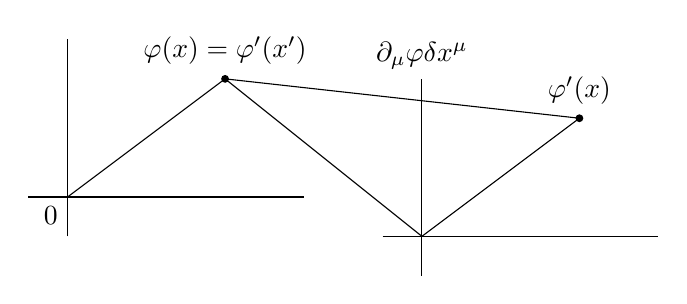
\begin{tikzpicture}
\draw (0,-.5) -- (0,2);
\draw (-.5,0) -- (3,0);
\draw (0,0) node[anchor=north east] {0};
\draw (0,0) -- (2,1.5) node[circle,fill,inner sep=1pt,label=above:{$\varphi(x)=\varphi'(x')$}]{};
\draw (4,-.5) -- (7.5,-.5);
\draw (4.5, -1) -- (4.5, 1.5) node[anchor=south]{$\partial_\mu\varphi\delta x^\mu$};
\draw (4.5,-.5) -- (6.5,1) node[circle,fill,inner sep=1pt,label=above:$\varphi'(x)$]{};
\draw (2,1.5) -- (4.5,-.5);
\draw (2,1.5) -- (6.5,1);
\end{tikzpicture}

\[ J^\mu_{(\nu)} = \pd{\mathcal{L}}{\partial_\mu\varphi}\partial_\rho\varphi - \eta^\mu_{\;\nu}\mathcal{L} \equiv \tilde{T}^\mu_{\;\nu} \]
\[ \tilde{T}^{\mu\nu} = \text{canonical energy-momentum tensor} \]
\[\begin{cases}
T^{\mu\nu} = \text{covariant EM tensor} \\
\tilde{T}^{\mu\nu} \text{is not symmetric $\mu\to\nu$}
\end{cases} \]

\[ Q_{(\nu)} \equiv \int \diff{^3x}\tilde{T}^{0}_{\;\nu} = \int \diff{^3x}\mathcal{P}_\nu \equiv P_\nu \]
 \[\begin{cases}
Q_{(0)} = \int \diff{^3x}\mathcal{P}_0 = \int \diff{^3x}\left(\pd{\mathcal{L}}{\partial_0\varphi}\partial_0\varphi - \mathcal{L}\right) \equiv \int \diff{^3x}\mathcal{H} = H \\
Q_{(i)} = \int \diff{^3x}\mathcal{P}_i = \int \diff{^3x}\pd{\mathcal{L}}{\partial_0\varphi}\partial_i\varphi
\end{cases}
\]

\subsubsection{Rotational invariance}
\[ \begin{cases}
x^{\prime\mu} = x^\mu + \omega^\mu_{\;\nu} x^\nu \\ \varphi'(x') = \varphi(x) - \frac{i}{2}\omega^{\mu\nu}\Omega_{\mu\nu}\varphi(x)
\end{cases} \qquad \to \qquad \begin{cases}
\delta x^\mu = \frac{1}{2}\omega^{\rho\sigma}\Xi^\mu_{(\rho\sigma)} \\ \delta \varphi = \frac{1}{2}\omega^{\rho\sigma}X_{(\rho\sigma)}
\end{cases} \]

\[ \begin{cases}
\Xi^\mu_{(\rho\sigma)} = \left(\eta^\mu_{\;\rho}\eta^\nu_{\;\sigma}-\eta^\mu_{\;\sigma}\eta^\nu_{\;\rho}\right)x^\rho \\
X_{(\rho\sigma)} = -i\Omega_{\rho\sigma}\varphi
\end{cases} \qquad \to \qquad \begin{cases}
\Omega_{\rho\sigma} = 0 \qquad (\text{scalar}) \\
\Omega_{\rho\sigma} = \Sigma'_{\rho\sigma} \qquad (\text{spinor})
\end{cases}\]

\[ J^\mu_{\rho\sigma} = \left(x_\rho\tilde{T}^\mu_\sigma - X_\sigma\tilde{T}^\mu_\rho\right) + S^\mu_{\rho\sigma} \]

\begin{align*}
Q_{(\rho\sigma)} &= \int \diff{^3x}J^0_{(\rho\sigma)} = \int \diff{^3x}\left[\left(x_\rho\mathcal{P}_\sigma - x_\sigma\mathcal{P}_\rho\right) + \mathcal{P}_{\rho\sigma}\right] \\
&= M_{\rho\sigma} = L_{\rho\sigma} + S_{\rho\sigma}
\end{align*}
Which is the external angular momentum plus the spin. ($x_\rho\mathcal{P}_\sigma - x_\sigma\mathcal{P}_\rho = \mathcal{L}_{\rho\sigma}$ and $\mathcal{P}_{\rho\sigma} = S^0_{\rho\sigma}$)

\section{Spin of a field}


\section{Dimensional analysis}
In the rest of part we set $c = 1 = \hbar $


\chapter{Canonical quantization}
It is now time to go from a classical to a quantum theory. This means quantization!
\section{Quantization}
\subsection{First quantization}
We start by exploring the quantization of a system with a finite number of degrees of freedom. We have already seen how to do this in the part on quantum mechanics. Here we give an alternative recipe (TODO: show that it is equivalent)
\[ \begin{cases}
p \equiv \pd{L}{\dot{q}} \\
H = p \; \dot{q} - L
\end{cases} \]
The equations of motion are given by the Poisson brackets
\[ \begin{cases}
\left\{q_i,p_j\right\}_t = \delta_{ij} \\ \left\{q_i,q_j\right\} = 0 = \left\{p_i,p_j\right\}
\end{cases} \qquad \begin{cases}
\dot{q}_i = \left\{q_i,H\right\}_t \\ \dot{p}_i = \left\{p_i, H\right\}_t
\end{cases}\]
We obtain the canonical quantization by applying the following substitutions:
\begin{itemize}
\item $(q_i, p_i)$ which are variables become $(X_i,P_i)$ which are operators;
\item $\{\;,\;\}_t \qquad \to \qquad - \frac{i}{\hbar}[\;,\;]_t$.
\end{itemize}
This gives us the following equations:
\[ \begin{cases}
[X_i,P_j]_t = i\hbar\delta_{ij} \\ [X_i,X_j] = 0 = [P_i,P_j]
\end{cases} \qquad \begin{cases}
\od{X_i}{t}  = - \frac{i}{\hbar}[X_i,H] \\ \od{P_i}{t} = - \frac{i}{\hbar}[P_i, H]
\end{cases} \]
As we can see, the operators evolve, so these are equations of motion in the Heisenberg picture.


For a finite number of degrees of freedom in momentum space we have $N$ independent oscillators.
\[ \begin{cases}
[a_p,a^\dagger_k] = \delta_{pk} \\
[a_p,a_k] = 0 = [a^\dagger_p, a^\dagger_k]
\end{cases} \]

(90\% of physics is harmonic oscillators because we expand to second order)



\subsection{Second quantization}
This procedure generalises quite nicely to fields with infinite degrees of freedom.
\[ \begin{cases}
\pi(x) \equiv \pd{\mathcal{L}}{\partial_0\varphi} \\ \mathcal{H} = \pi\cdot\partial_0\varphi - \mathcal{L}
\end{cases} \]
The Poisson brackets:
\[ \begin{cases}
\left\{\varphi(\overline{x},t),\pi(\overline{y},t)\right\}_t = \delta^3(\overline{x}- \overline{y}) \\ \left\{\varphi(\overline{x},t),\varphi(\overline{y},t)\right\}_t = 0 = \left\{\pi(\overline{x},t),\pi(\overline{y},t)\right\}_t
\end{cases} \qquad \begin{cases}
\dot{\varphi}(\overline{x},t) = \left\{\varphi(\overline{x},t),H\right\}_t \\ \dot{\pi}(\overline{x},t) = \left\{\pi(\overline{x},t), H\right\}_t
\end{cases}\]
The quantization given by following substitution:
\begin{itemize}
\item $(\varphi, \pi)$ = classical fields $\to$ $(\hat{\varphi}, \hat{\pi})$ = operator fields
\item $\{\;,\;\}_t \qquad \to \qquad -i[\;,\;]_t \qquad (\hbar = 1 =c)$
\end{itemize}
This gives us the following quantization:
\[ \begin{cases}
\left[\hat{\varphi}(\overline{x},t), \hat{\pi}(\overline{y},t)\right]_t = i\delta^3(\overline{x}- \overline{y}) \\
\left[\hat{\varphi}(\overline{x},t)\hat{\varphi}(\overline{y},t)\right]_t = 0 = \left[\hat{\pi}(\overline{x},t), \hat{\pi}(\overline{y},t)\right]_t
\end{cases} \qquad \begin{cases}
\dot{\hat{\varphi}}(\overline{x},t) = -i \left[\hat{\varphi}(\overline{x},t), \hat{H}\right]_t \\
\dot{\hat{\pi}}(\overline{x},t) = -i \left[\hat{\pi}(\overline{x},t), \hat{H}\right]_t
\end{cases}\]



In momentum space we get an equivalent quantization condition:
\[ \begin{cases}
\left[a(p), a^\dagger(k)\right] = \delta^3(\vec{p}- \vec{k}) \\
\left[a(p),a(k)\right] = 0 = \left[a^\dagger(p), a^\dagger(k)\right]
\end{cases} \]
Which is a continuous set of uncoupled harmonic oscillators.

\section{Number (density) operator}
TODO see p5-6 in Mandl-Shaw

The \udef{number density operator}
\[ \mathcal{N}(k) \equiv a^\dagger(k)a(k)\]
has the following properties

\begin{eigenschap}
\begin{itemize}
\item  $\mathcal{N}(k)^\dagger = \mathcal{N}(k)$
\item \raisebox{-0.95em}{$\begin{aligned}
&[\mathcal{N}(k), a(p)] = -a(p)\delta^3(\overline{k}- \overline{p}) \\
&[\mathcal{N}(k), a^\dagger(p)] = +a^\dagger(p)\delta^3(\overline{k}- \overline{p})
\end{aligned}$}
\end{itemize}
\end{eigenschap}


The \udef{number operator}
\[ N \equiv \int \diff{^3k}\mathcal{N}(k)\]
has the following properties
\begin{eigenschap}
\begin{itemize}
\item  $N^\dagger = N$
\item \raisebox{-0.95em}{$\begin{aligned}
&[N, a(p)] = -a(p) \\
&[N, a^\dagger(p)] = +a(p)
\end{aligned}$}
\end{itemize}
\end{eigenschap}

\section{Normal ordering}

\section{What are the states in QFT?}
So far we have operator fields, but no states. The space of states in quantum field theory is called the \udef{Fock Space}.
\subsection{Postulate of the existence of vacuum $=\ket{0}$}
\[ \boxed{a(k)\ket{0}=0} \qquad \forall k \]
\[ \begin{cases}
\mathcal{N}(k)\ket{0} = 0 \qquad \to \qquad 0\; \text{occupation number} \\
N[H]\ket{0} = 0 \qquad \to \qquad 0\; \text{energy, momentum}
\end{cases} \]

\subsection{The Fock space}(Hilbert space) is the space with \ueig{all possible states} generated by applying $a^\dagger(k)$ on $\ket{0}$. So a generic state in Fock space can be written as
\[ \ket{n_1(k_1), \ldots, n_l(k_l)}\quad \sim \quad a^\dagger(k_1)^{n_1} \ldots a^\dagger(k_l)^{n_l} \ket{0} \]

\begin{example}
We consider the simplest non vacuum state $\ket{1(k)} \sim a^\dagger(k)\ket{0}$.
\begin{align*}
N\ket{1(k)} &\sim \int \diff{^3p}\mathcal{N}(p)a^\dagger(k)\ket{0} \\
&= \int \diff{^3p}\left([\mathcal{N}(p),a^\dagger(k)] + a^\dagger(k)\mathcal{N}(p)\right)\ket{0} \\
&= \int \diff{^3p} \delta^3(k-p)a^\dagger(k)\ket{0} + \cancel{a^\dagger(p)\mathcal{N}(k)\ket{0}} \\
&= \int \diff{^3p} \left(1\delta^3(k- p)a^\dagger(p) + \cancel{a^\dagger(p)\mathcal{N}(k)}\right)\ket{0} \\
&\sim +1 \ket{1(k)}
\end{align*}
Similarly
\[ \begin{cases}
H\ket{1(k)} = \omega_k\ket{1(k)} \qquad \text{where} \qquad \omega_k = \left(m^2 + |\overline{k}|^2\right)^{1/2} \\
P\ket{1(k)} = k\ket{1(k)}
\end{cases} \]
From this we get for a state of $n$ identical particles
\begin{align*}
\ket{n(k)} &\sim a^\dagger(k)^n\ket{0}\\
N\ket{n(k)} &= n\ket{n(k)} \\
H\ket{n(k)} &= n\omega_k\ket{n(k)}\\
\overline{P}\ket{n(k)} &= n \overline{k} \ket{n(k)}
\end{align*}
Also
\begin{align*}
\ket{n_1(k_1), n_2(k_2)} &\sim a^\dagger(k_1)^{n_1}a^\dagger(k_2)^{n_2}\ket{0}\\
N\ket{n_1(k_1), n_2(k_2)} &= (n_1+n_2)\ket{n_1(k_1), n_2(k_2)} \\
H\ket{n_1(k_1), n_2(k_2)} &= (n_1\omega_1+n_2\omega_2)\ket{n_1(k_1), n_2(k_2)} \\
P\ket{n_1(k_1), n_2(k_2)} &= (n_1k_1+n_2k_2)\ket{n_1(k_1), n_2(k_2)}
\end{align*}
\end{example}

From this example we learn that the Fock space of a real scalar field corresponds to a particle with Bose statistics, as we can add as many identical particles as we want.
\begin{eigenschap}
Scalar field corresponds to spin 0
\end{eigenschap}

\subsection{Normalization of states}
\[ \braket{1(p)}{1(k)} = \delta^3(\overline{k}- \overline{p}) \]


Firstly
\[\braket{0}{0} = 1\]
Normally we would normalize the states as follows
\[ \begin{cases}
\ket{1(k)} = a^\dagger(k)\ket{0} \\
\braket{1(p)}{1(k)} = \delta^3(\overline{k}- \overline{p})
\end{cases}\]
This normalisation is not invariant under Lorentz transformations however.

So we use the ``good'' normalization
\[ \begin{cases}
\ket{1(k)} = (2\pi)^{3/2}\sqrt{2\omega_k}a^\dagger(k)\ket{0} \\
\braket{1(p)}{1(k)} = (2\pi)^{3}2\omega_k\delta^3(\overline{k}- \overline{p})
\end{cases} \]

\section{Covariant commutators and propagators}
\subsection{Feynman propagator}

\begin{definition}
The \udef{Feynman propagator} $\Delta_F$ is defined as
\[ \Delta_F(x-y) \equiv \expval{T \left(\varphi(x)\varphi(y)\right)}{0} = \varphi(x)\varphi(y) \]
\end{definition}
\begin{align*}
\Delta_F(x-y) &= \theta(x_0-y_0)\expval{T \left(\varphi(x)\varphi(y)\right)}{0} + \theta(y_0-x_0)\expval{T \left(\varphi(x)\varphi(y)\right)}{0} \\
&= \theta(x_0-y_0)\expval{T \left(\varphi_+(x)\varphi_-(y)\right)}{0} + \theta(y_0-x_0)\expval{T \left(\varphi_+(x)\varphi_-(y)\right)}{0} \\
&= \theta(x_0-y_0)\expval{[\varphi_+(x), \varphi_-(y)]}{0} - \theta(y_0-x_0)\expval{[\varphi_-(x), \varphi_+(y)]}{0} \\
&= \theta(x_0-y_0)D_+(x-y) - \theta(y_0-x_0)D_-(x-y)
\end{align*}
The following relation holds
\[ T \left(\varphi(x)\varphi(y)\right) = N\left(\varphi(x)\varphi(y)\right) + \varphi(x)\varphi(y)  \]
\begin{align*}
\varphi(x)\varphi(y) = T\left(\varphi(x)\varphi(y)\right) - N\left(\varphi(x)\varphi(y)\right) \\
&= \theta(x_0-y_0)\left(\cancel{\varphi_-(x)\varphi_-(y)}+\xcancel{\varphi_+(x)\varphi_+(y)}+\bcancel{\varphi_-(x)\varphi_+(y)}+\varphi_+(x)\varphi_-(y)\right) + \theta(y_0-x_0)\left(\cancel{\varphi_-(y)\varphi_-(x)}+\xcancel{\varphi_+(y)\varphi_+(x)}+\varphi_+(y)\varphi_-(x)+\bcancel{\varphi_-(y)\varphi_+(x)}\right) \\
- \theta(x_0-y_0)\left(\cancel{\varphi_-(x)\varphi_-(y)}+\xcancel{\varphi_+(x)\varphi_+(y)}+\bcancel{\varphi_-(x)\varphi_+(y)}+\varphi_-(y)\varphi_+(x)\right) - \theta(y_0-x_0)\left(\cancel{\varphi_-(x)\varphi_-(y)}+\xcancel{\varphi_+(x)\varphi_+(y)}+\varphi_-(x)\varphi_+(y)+\bcancel{\varphi_-(y)\varphi_+(x)}\right)
&= \theta(x_0 - y_0)\left[\varphi_+(x),\varphi_-(y)\right] - \theta(y_0-x_0)\left[\varphi_-(x),\varphi_+(y)\right] \\
&= \theta(x_0 - y_0)D_+(x-y) - \theta(y_0-x_0)D_-(x-y)
\end{align*}


\begin{definition}
The \udef{Feynman propagator} (complex scalar)
\begin{align*}
\Delta_F(x-y) &\equiv \expval{T \left(\varphi(x)\varphi^\dagger(y)\right)}{0} = \underbrace{\varphi(x)\varphi^\dagger(y)} \\
&= \theta(x_0-y_0)D_+(x-y) - \theta(y_0-x_0)D_-(x-y)
\end{align*}
\end{definition}

\begin{definition}
The \udef{Feynman propagator for Dirac fields}
\begin{align*}
S^{\alpha\beta}_+(x-y) &\equiv \expval{T \left(\psi_{\alpha}(x)\overline{\psi}_{\beta}(y)\right)}{0} = \underbrace{\psi_{\alpha}(x)\overline{\psi}_{\beta}(y)} \\
&= \theta(x_0-y_0)S_+^{\alpha\beta}(x-y) - \theta(y_0-x_0)S^{\alpha\beta}_-(x-y) \\
&= (i\slashed{\partial}+m)D_F(x-y)
\end{align*}
\remark{Ex.}
\end{definition}


\subsection{Time-ordered product}
\begin{definition}
The \udef{time-ordered product} of two operators $A$ and $B$
\[ T \left(A(t_1)B(t_2)\right) = \begin{cases}
A(t_1)B(t_2) & (t_1 > t_2) \\
\pm B(t_2)A(t_1) & (t_1 < t_2)
\end{cases} \]
Where the $\pm$ is $+$ for bosons and $-$ for fermions. For $n$ operators, the time-ordered product orders them by time and introduces a factor $(-1)^p$ where $p$ is the number of fermionic exchanges necessary to achieve time ordering.

The time-ordered product is also taken to be linear, if addition were to turn up in the product.
\end{definition}

\subsection{Introducing Feynman diagrams}
integral over time, no time ordering. time left to right. arrows and momenta

\subsection{Microcausality}

\section{Spin statistics theorem}
\subsection{Quantization with anti-commutators}

\chapter{Some examples of quantum field theories}
We want an explicit expression for the Lagrangian density. We will try to guess its form.
\begin{enumerate}
\item The action is more or less an observable so we want it to be real (Hermitian)
\remark{$\mathcal{L} = $ real (Hermitian)}
\item The action is a scalar (under Poincaré transformation)
\remark{$\mathcal{L} = $ scalar density}
\item The action is adimensional in natural units
\[ \hookrightarrow S = \int \diff{^4x}\mathcal{L} = [M]^{-4}[M]^4 = [M]^0 \]
\item By equation of motion $\to$ relativistic equation = nice
\[ \mathcal{L}(\varphi, \partial_\mu\varphi) \]
\end{enumerate}


\section{Klein-Gordon field (real scalar field)}


As a first example, we consider the following Lagrangian for a real scalar field:
\[ \mathcal{L} = \frac{1}{2}(\partial_\mu\varphi)(\partial^\mu\varphi) - \frac{1}{2}m^2\varphi^2 \]
where $m$ is a parameter that we will identify with the mass.
This can be seen as the sum of kinetic and a mass term (TODO why?). Knowing that the Lagrangian must have a dimension of $[M^4]$ and that each derivative has dimension $[\partial] = [M^1]$, we see that
\[ \begin{cases}
[\varphi] = [M^1] \\
[m] = [M^1]
\end{cases} \]
Luckily this is consistent with our identification of $m$ as the mass.

Because we are dealing with a real and relativistic field, we impose the following conditions
\[ \begin{cases}
\varphi(x) = \varphi^*(x) \\
\varphi'(x') = \varphi(x)
\end{cases} \]
where the prime means the quantity has been transformed by a Poincaré transformation.

\subsection{Equation of motion}
Applying the Euler-Lagrange equation
\[ \pd{\mathcal{L}}{\varphi} - \partial_\mu \pd{\mathcal{L}}{\partial_\mu\varphi} = 0 \]
We get the Klein-Gordon equation:
\[ -m^2\varphi - \partial_\mu\partial^\mu\varphi = -(\Box+m^2)\varphi = 0\]
As we know this has the following general solution:
\[ \varphi(x) = \frac{1}{(2\pi)^{3/2}}\int \diff{^3k}\left(a(k)e^{-ikx} + a^*(k)e^{ikx}\right)_{k_0 = \omega_k} \]

\subsection{Hamiltonian formulation}
We now calculate the relevant quantities in the Hamiltonian formulation.
\[ \pi \equiv \pd{\mathcal{L}}{\partial_0\varphi} = \frac{1}{2}(\partial_0 \varphi + \partial^0 \varphi) = \partial_0 \varphi \]
\[ \mathcal{H} = \pi \partial_0\varphi - \mathcal{L} = \frac{1}{2}\pi^2 + \frac{1}{2}(\overline{\nabla}\varphi)^2 + \frac{1}{2}m^2\varphi^2 \]
We see that the Hamiltonian density is always positive. (TODO: as opposed to ...)
\[ H = \int \diff{^3x}\mathcal{H} > 0 \]

\begin{example}
Exercise: Verify Poisson Brackets
\begin{align*}
\dot{\varphi} &= \left\{\varphi(\overline{x},t), H\right\}_t \\
\dot{\pi} &= \left\{\pi(\overline{x},t), H\right\}_t
\end{align*}
\[ \left\{\varphi(\overline{x},t), \varphi(\overline{y},t)\right\} = 0 \]
\end{example}

\subsection{Symmetries}
\subsubsection{Translational invariance}
\[J^\mu_{(\nu)} = (\partial^\mu\varphi)(\partial_\nu\varphi) - \eta^\mu_{\;\nu}\mathcal{L}\]
\[ \partial_\mu J^\mu_{(\nu)} = 0 \qquad \to \qquad \text{Exercise: prove} \]
The 4 conserved charges:
\[\begin{cases}
P_0 \equiv H = \int \diff{^3x}\left\{\pi\partial_0\varphi-\mathcal{L}\right\} = \int \diff{^3x}\mathcal{H} \\
P_i = \int \diff{^3x}\mathcal{P}_i = \int \diff{^3x} \pi(\partial_i\varphi)
\end{cases}\]

\subsubsection{Rotational invariance}

\[\begin{cases}
\delta x^\mu = \omega^{\rho\sigma}\Xi^\mu_{(\rho\sigma)} \qquad \to \qquad \Xi^\mu_{(\rho\sigma)} = \left(\eta^\mu_{\;\rho}\eta^\nu_{\;\sigma}-\eta^\mu_{\;\sigma}\eta^\nu_{\;\rho}\right)x^\nu \\
\delta \varphi = \frac{1}{2}\omega^{\rho\sigma}X_{(\rho\sigma)} = 0 \qquad \to \qquad X_{(\rho\sigma)} = 0
\end{cases} \]
Differences??
\[ \frac{1}{2},\nu \text{ipv} \rho \]

\[ J^\mu_{(\rho\sigma)} = \left(x_\rho\tilde{T}^\mu_{\;\sigma} - x_\sigma\tilde{T}^\mu_{\;\rho}\right) + (X) \]

\begin{align*}
Q_{(\rho\sigma)} &= \int \diff{^3x}J^0_{(\rho\sigma)} = \int \diff{^3x}\left(x_\rho\mathcal{P}_\sigma - x_\sigma\mathcal{P}_\rho\right) =L_{(\sigma\rho)??\text{(last equality)}}
\end{align*}

\begin{example}
Exercise: Write $P^\mu$ in the momentum space (as functions of $a(k), a^*(k)$)

Solution:
\[\varphi(x) = \frac{1}{(2\pi)^{3/2}}\int \frac{\diff{^3k}}{\sqrt{2\omega_k}}\left(a(k)e^{-ikx}+a^*(k)e^{ikx}\right)_{k_0 = \omega_k} \]
\begin{align*}
H &= \frac{1}{2} \int \diff{^3x}\left(\pi^2 + (\overline{\nabla})^2 m^2\varphi^2\right) \\
&= \frac{1}{2}\int \frac{\diff{^3x}}{(2\pi)^3}\int \frac{\diff{^3k}\diff{^3p}}{\sqrt{4\omega_k\omega_p-\omega_k}} \times \left\{(-i\omega_k)(-i\omega_p)\left[a(k)a(p)e^{-i(k+p)x}+a^*(k)a^*(p)e^{i(k+p)x}-a(k)a^*(p)e^{-i(k-p)x}-a^*(k)a(p)e^{i(k-p)x}\right] + (i \overline{k})(i \overline{p})\left[a(k)a(p)e^{-i(k+p)x}+a^*(k)a^*(p)e^{i(k+p)x}-a(k)a^*(p)e^{-i(k-p)x}-a^*(k)a(p)e^{i(k-p)x}\right] + m^2 \left[a(k)a(p)e^{-i(k+p)x}+a^*(k)a^*(p)e^{i(k+p)x}-a(k)a^*(p)e^{-i(k-p)x}-a^*(k)a(p)e^{i(k-p)x}\right] \right\} \\
&= \frac{1}{2} \int \frac{\diff{^3k}\diff{^3p}}{\sqrt{4\omega_k\omega_p-\omega_k}}
\int \frac{\diff{^3x}}{(2\pi)^3} \left\{(m^2-\omega_k\omega_k - \overline{k}\cdot\overline{p})
\left[a(k)a(p)e^{-i(k+p)x}+a^*(k)a^*(p)e^{i(k+p)x}\right]
+ \left[a(k)a^*(p)e^{-i(k-p)x}+a^*(k)a(p)e^{i(k-p)x}\right] \right\}
\end{align*}
Let's integrate $\int \diff{^3x}$:
\[H = \frac{1}{2}\int \frac{\diff{^3k}\diff{^3p}}{\sqrt{4\omega_k\omega_p}} \left\{ \delta^3(\overline{k}+\overline{p})(m^2-\omega_k\omega_p - \overline{k}\cdot \overline{p})\left[ a(k)a(p)e^{-i(k_0+p_0)x_0} + a^*(k)a^*(p)e^{+i(k_0+p_0)x_0} \right] + \delta^3(\overline{k}-\overline{p})(m^2+\omega_k\omega_p + \overline{k}\cdot \overline{p})\left[ a(k)a^*(p)e^{-i(k_0-p_0)x_0} + a^*(k)a(p)e^{+i(k_0-p_0)x_0} \right] \right\}\]
Let's integrate $\int \diff{^3p}$:
\begin{align*}
H &= \frac{1}{2}\int \frac{\diff{^3k}}{2\omega_k} \left\{ (m^2-\omega_k^2 - |\overline{k}|^2)\left[ \ldots \right] + (m^2+\omega_k^2 + |\overline{k}|^2)\left[ a(k)a^*(p) + a^*(k)a(p) \right] \right\} \\
&=\frac{1}{2} \int \diff{^3k}\omega_k(a(k)a^*(k)+a^*(k)a(k))
\end{align*}
We didn't use any ``commutator property''
\[ \boxed{H = \int \diff{^3k}\omega_ka^*(k)a(k)} \qquad \text{total energy} \]
\begin{align*}
P^i &= \int \diff{^3k} k^i(a(k)a^*(k) + a^*(k)a(k)) \\
\Aboxed{P^i &= \int \diff{^3 k}k^ia^*(k)a(k)} \qquad \text{total free momentum}
\end{align*}

\end{example}

\subsection{Quantization}

Following the recipe for the second quantization (TODO ref), we get
\[ \begin{cases}
\left[\hat{\varphi}(\vec{x},t), \hat{\pi}(\vec{y},t)\right]_t = i\delta^3(\vec{x}- \vec{y}) \\
\left[\hat{\varphi}(\vec{x},t)\hat{\varphi}(\vec{y},t)\right]_t = 0 = \left[\hat{\pi}(\vec{x},t), \hat{\pi}(\vec{y},t)\right]_t
\end{cases} \]

We have already shown that the solutions of the Klein-Gordon equation are of the form 
\[ \begin{cases}
\hat{\varphi}(x) = \frac{1}{(2\pi)^{3/2}} \int \frac{\diff{^3k}}{\sqrt{2\omega_k}} \left(\hat{a}(k)e^{-ikx} + \hat{a}^\dagger(k)e^{ikx}\right)_{k_o=\omega_k} \\
\hat{\pi}(x) = \frac{-i}{(2\pi)^{3/2}} \int \frac{\diff{^3k}}{\sqrt{2\omega_k}} \omega_k \left(\hat{a}(k)e^{-ikx} - \hat{a}^\dagger(k)e^{ikx}\right)_{k_o=\omega_k}
\end{cases} \]
where the integral is over all wave vectors allowed by the boundary conditions.
Alternatively, we can write in momentum space
\[ \begin{cases}
\hat{a}(p) = \left. \frac{1}{(2\pi)^{3/2}} \int \frac{\diff{^3x}}{\sqrt{2\omega_p}} \left(\omega_p\varphi(\vec{x},t)+i\pi(\vec{x},t)\right)e^{ipx}\right|_{p_o=\omega_p} \\
\hat{a}^\dagger(p) = \left. \frac{1}{(2\pi)^{3/2}} \int \frac{\diff{^3x}}{\sqrt{2\omega_p}} \left(\omega_p\varphi(\vec{x},t)-i\pi(\vec{x},t)\right)e^{-ipx}\right|_{p_o=\omega_p}
\end{cases} \]

In momentum space we get an equivalent quantization condition:
\[ \begin{cases}
\left[a(p), a^\dagger(k)\right] = \delta^3(\vec{p}- \vec{k}) \\
\left[a(p),a(k)\right] = 0 = \left[a^\dagger(p), a^\dagger(k)\right]
\end{cases} \]
These are the harmonic oscillator commutation relations for a continuous set of uncoupled harmonic oscillators.


\subsection{Hamiltonian (density)}
The \udef{Hamiltonian density operator}
\[ \mathcal{H}(\varphi, \pi) \equiv \frac{1}{2}\pi^2 + \frac{1}{2}(\overline{\nabla}\varphi)^2 + \frac{1}{2}m^2\varphi^2 \]
The \udef{Hamiltonian operator}
\begin{align*}
H &= \int \diff{^3x}\mathcal{H} = \frac{1}{2}\int\diff{^3k}\omega_k \left(a^\dagger(k)a(k) + a(k)a^\dagger(k)\right) \\
&= \int\diff{^3k}\omega_k \left(a^\dagger(k)a(k) + \frac{1}{2}[a(k),a^\dagger(k)]\right) \\
&= \underbrace{\int \diff{^3k}\omega_k\mathcal{N}(k)}_{\Delta E \text{energy operator}} + \xcancel{\frac{1}{2}\int \diff{^3k}\omega_k\delta^3(\overline{k}- \overline{k})}
\end{align*}
\[ N[H] = \int \diff{^3k}\omega_k\mathcal{N}(k) \]

The dropped term corresponds to the constant energy of vacuum ($E_0 \;\to\; \infty$). We drop it here because it is constant (i.e. a number, not an operator), but it becomes relevant when quantizing gravity.

\subsection{Three momentum (density) operator}
\begin{align*}
P_i &= \int \diff{^3x}\pi(\partial_i\varphi) = \ldots \\
&= \frac{1}{2}\int \diff{^3k}(k_i)\left(a^\dagger(k)a(k)+ a(k)a^\dagger(k)\right) \\
&= \int \diff{^3k} k_i \mathcal{N}(k) + \xcancel{\infty -\text{number}}
\end{align*}
\[ N[P_i] = \int \diff{^3k} k_i \mathcal{N}(k) \]

The switching round of $a(k)$ and $a^\dagger(k)$ in the previous calculations motivates us to make the following definition:
\begin{definition}
A product is \udef{normal ordered} when all creation operators are to the left of all annihilation operators in the product. I.e. when all $a^\dagger$ are on the left and all $a(k)$ are on the right
\[ N[a^\dagger(k)a(k) + a(k)a^\dagger(k)] = 2 a^\dagger(k)a(k) \]
Inside $N[\;]$ (for scalar fields) everything commutes.
\end{definition}
\remark{Normal ordering does not touch any H.O. commutators}

\subsection{General solution and interpretation}


From now on we drop the hats over the operators to make the notation less heavy. We also split 
\begin{align*}
\varphi(x) &= \frac{1}{(2\pi)^{3/2}} \int \frac{\diff{^{3}k}}{\sqrt{2\omega_k}}\left(a(k)e^{-ikx} + a^\dagger(k)e^{ikx}\right)_{k_0 = \omega_k} \\
&= \varphi_+(x) + \varphi_-(x)
\end{align*}
The operators $\varphi_\pm(x)$ are the annihilation / creation operators of a particle with only momentum $k$ at the point $x$.

One-particle states are linear superpositions of
\[ a^\dagger(\vec{k})\ket{0} \qquad\text{for any}\qquad \vec{k} \]
Two-particle states are linear superpositions of
\[ a^\dagger(\vec{k})a^\dagger(\vec{k'})\ket{0} \qquad\text{for any}\qquad  \vec{k}, \vec{k'} \neq \vec{k} \]
and
\[ \frac{1}{\sqrt{2}}(a^\dagger(\vec{k}))^2\ket{0} \qquad\text{for any}\qquad  \vec{k} \]

These states are normalized if the vacuum state is normalized.
\begin{example}
\begin{align*}
\bra{0}\left(\varphi_+(x)\ket{1(p)}\right) &= \frac{1}{(2\pi)^{3/2}} \int \frac{\diff{^{3}k}}{\sqrt{2\omega_k}}(2\pi)^{3/2}\sqrt{2\omega_p}\braket[a(k)a^\dagger(p)]{0}{0}e^{-ikx} \\
&= \int \diff{^3k}\frac{\sqrt{2\omega_p}}{\sqrt{2\omega_k}}\delta^3(\overline{k} - \overline{p})e^{-ikx}\braket{0}{0} = e^{-ipx}
\end{align*}
\end{example}
(This example also hints at the reason why the ``good'' normalization is good)


\subsection{Covariant commutators}
So far the story has been:
\begin{enumerate}
\item We defined the Lagrangian density, $\mathcal{L}$, which is a \ueig{covariant} object.
\item We then switched to the Hamiltonian formalism, with $\mathcal{H} = \pi\partial_0\varphi - \mathcal{L}$. This is the Legendre transformation of the Lagrangian density. The Hamiltonian density $\mathcal{H}$ is not manifestly covariant. (Which is why we stressed that we compute it at fixed time)
\item We then applied the canonical quantization to get $[\varphi(\overline{x},t), \pi(\overline{y},t)] = i\delta^3(\overline{x}- \overline{y})$, which is not manifestly covariant.
\end{enumerate}
So we need now to verify that the canonical quantization is consistent with Lorentz covariance.
In other words, we need to show that the commutation relations are covariant. 
To do that, we write the commutator $[\varphi(x), \varphi(y)]$ for two arbitrary spacetime points $x$ and $y$.

First we note that
\[ [\varphi_+(x),\varphi_+(y)] = [\varphi_-(x),\varphi_-(y)] = 0. \]
So
\begin{align*}
[\varphi(x), \varphi(y)] &= [\varphi_+(x)+\varphi_-(x), \varphi_+(y) + \varphi_-(y)] \\
&= [\varphi_+(x), \varphi_-(y)] + [\varphi_-(x), \varphi_+(y)] \\
&\equiv D_+(x,y) + D_-(x,y)
\end{align*}
Working out each part separately, we get
\begin{align*}
D_+(x,y) &\equiv [\varphi_+(x), \varphi_-(y)]\\
&= \frac{1}{(2\pi)^{3}} \int \frac{\diff{^{3}k}}{\sqrt{2\omega_k}} \int \frac{\diff{^{3}k'}}{\sqrt{2\omega_{k'}}} e^{-ikx}e^{ik'y}\left[a(k), a^\dagger(k')\right] \\
&= \left.\frac{1}{(2\pi)^{3}} \int \frac{\diff{^{3}k}}{2\omega_k} e^{-ik(x-y)}\right|_{k_0 = \omega_k}
\end{align*}
and
\begin{align*}
D_-(x,y) &\equiv [\varphi_-(x), \varphi_+(y)]\\
&= \frac{1}{(2\pi)^{3}} \int \frac{\diff{^{3}k}}{\sqrt{2\omega_k}} \int \frac{\diff{^{3}k'}}{\sqrt{2\omega_{k'}}} e^{ikx}e^{-ik'y}\left[a^\dagger(k), a(k')\right] \\
&= -\left.\frac{1}{(2\pi)^{3}} \int \frac{\diff{^{3}k}}{2\omega_k} e^{ik(x-y)}\right|_{k_0 = \omega_k}
\end{align*}
We notice that $D_+$ and $D_-$ do not really depend on both $x$ and $y$, but rather on their difference $x-y$. Thus we can define
\begin{align*}
D(x-y) &\equiv D_+(x-y) + D_-(x-y) \\
&= \left.\frac{1}{(2\pi)^3}\int \frac{\diff{^3k}}{2\omega_k}\left( e^{-ik(x-y)} - e^{ik(x-y)} \right)\right|_{k_0=\omega_k} \\
&= - \left.\frac{1}{(2\pi)^3}\int \frac{\diff{^3k}}{\omega_k}\sinh(x-y)\right|_{k_0=\omega_k}
\end{align*}


We can now write $D_\pm(x-y)$ in a covariant way:
\[ D_\pm(x-y) \equiv i \int_{c_\pm}\frac{\diff{^4k}}{(2\pi)^4}\frac{e^{-ik(x-y)}}{k^2-m^2} \]



Let's calculate $D_+(x-y)$
\begin{align*}
D_+(x-y) &= \frac{i}{(2\pi)^4}\int_{c_+}\diff{^4k}\frac{e^{-ik(x-y)}}{k^2-m^2} \\
&= i \int \frac{\diff{^3k}}{(2\pi)^3}e^{i \overline{k}(\overline{x}- \overline{y})} \cdot \int_{c_+} \frac{\diff{k_0}}{2\pi} \frac{e^{ik_0(x_0-y_0)}}{(k_0-\omega_k)(k_0+\omega_k)}
\end{align*}
We define
\[ f(k_0) = \frac{e^{ik_0(x_0-y_0)}}{2\pi(k_0-\omega_k)(k_0+\omega_k)} \]
Now, using the residue theorem
\begin{eigenschap}
\ueig{Residue theorem}
\[ \int_{c_+}\diff{k_0}f(k_0) = -2\pi i \Res(f(k_0))_{k_0=\omega_k} \]
\end{eigenschap}

\begin{figure}
\centering
\begin{tikzpicture}
\draw[->] (-3,0) -- (3,0) node[anchor=west]{$\text{Re}\,k_0$};
\draw[->] (0,-1.5) -- (0,1.5) node[anchor=south]{$\text{Im}\,k_0$};
\draw (-1.5,0) node[circle,fill,inner sep=1pt, label=below:$-\omega_k$]{};
\draw (1.5,0) node[circle,fill,inner sep=1pt, label=below:$+\omega_k$]{};
\draw[decoration={markings, mark=at position 0.25 with {\arrow{<}}, markings, mark=at position 0.75 with {\arrow{<}}}, postaction={decorate}] (-1.5,0) circle (.7);
\draw[decoration={markings, mark=at position 0.25 with {\arrow{<}}, markings, mark=at position 0.75 with {\arrow{<}}}, postaction={decorate}] (1.5,0) circle (.7);
\draw (2,.5) node[anchor=south west] {$\mathcal{C}_+$};
\draw (-2,.5) node[anchor=south east] {$\mathcal{C}_-$};
\end{tikzpicture}
\end{figure}

we get
\[D_+(x-y) = i \int \frac{\diff{^3k}}{(2\pi)^3}(-2\pi i) \frac{e^{-i\omega_k(x_0-y_0)}}{(2\pi)2\omega_k}e^{i \overline{k}(\overline{x} - \overline{y})} = \left.\frac{1}{(2\pi)^3}e^{-ik(x-y)}\right|_{k_0=\omega_k} \]

In conclusion the quantization conditions are consistent with covariance of the theory
\[ D(x-y) = [\varphi(x), \varphi(y)] \]
\begin{example}
Exercise: $[\pi(x), \pi(y)], [\varphi(x), \pi(y)]$
\end{example}

\subsection{Covariance and causality}
\begin{itemize}
\item $D(x-y) \equiv [\varphi(x),\varphi(y)]$ is covariant.
\item $\left.D(x-y)\right|_{x_0=y_0} = [\varphi(x,t), \varphi(y,t)] = 0$

So $D(x-y) = 0$ if $(x-y)^2<0$ (space line)
\end{itemize}

The creation / annihilation of a particle $(x_0, \overline{x})$ cannot be influenced by the creation / annihilation of a particle $(y_0,\overline{y})$ if $(x-y)^2<0$

Given $A,B$; if $[A,B] = 0$ there is no interference in the measurement

Microcausality.

Lecture 5/11

Recap
Canonical quantization of complex scalar (free)
\begin{enumerate}
\item General form
\begin{align*}
\varphi(x) = \frac{1}{(2\pi)^{3/2}} \int \frac{\diff{^3k}}{2\omega_k}() \equiv \varphi_+(x)+\varphi_-(x)\\
\end{align*}
?
\item Hamiltonian formalism
\begin{align*}
\pi &\equiv \pd{\mathcal{L}}{\partial_0\varphi} = \partial_0\varphi^\dagger \qquad \to \qquad (\varphi, \pi) \\
\pi^\dagger &\equiv \pd{\mathcal{L}}{\partial_0\varphi^\dagger} = \partial_0\varphi \qquad \to \qquad (\varphi^\dagger, \pi^\dagger)
\end{align*}
\[\mathcal{H} = \pi\partial_0\varphi + \pi^\dagger\partial_0\varphi^\dagger - \mathcal{L}\]
\item Canonical quantization
\begin{align*}
[\varphi(\overline{x},t), \pi(\overline{y},t)]_t &= i\delta^3(\overline{x}- \overline{y}) = [\varphi^\dagger(\overline{x},t), \pi^\dagger(\overline{y},t)] \\
[\varphi(\overline{x},t),\varphi(\overline{y},t)] &=0 = [\varphi^\dagger(\overline{x},t),\varphi^\dagger(\overline{y},t)] = \ldots
\end{align*}
So equations of motion (Heisenberg picture)
\[ \od{\varphi^{(\dagger)}(\overline{x},t)}{t} = -i[\varphi^{(\dagger)}(\overline{x},t),H], \qquad \od{\pi^{(\dagger)}(\overline{x},t)}{t} = -i[\pi^{(\dagger)}(\overline{x},t),H] \]
\item Quantization conditions in momentum space
\begin{align*}
[a(p), a^\dagger(k)] &= \delta^3(\overline{p}- \overline{k}) &= [b(p), p^\dagger(k)] \\
[a^{(\dagger)}(p), a^{(\dagger)}(k)] &= 0 &= [b^{(\dagger)}(p), b^{(\dagger)}(k)]
\end{align*}
So there are two sets of infinite ($\forall k$) H.O. (decoupled)
\item Observables
\[ \begin{cases}
\mathcal{N_a}(k) \equiv a^\dagger(k)a(k) \qquad N_a \equiv \int \diff{^3k}\mathcal{N_a}(k) \\
\mathcal{N_b}(k) \equiv b^\dagger(k)b(k) \qquad N_b \equiv \int \diff{^3k}\mathcal{N_b}(k)
\end{cases} \]
\begin{align*}
N[H] &\equiv \int \diff{^3x}\mathcal{H} = \int \diff{^3k}\omega_k \left(\mathcal{N}_a(k) + \mathcal{N}_b(k)\right) \qquad \geq 0 \\
N[Q] &\equiv q\int \diff{^3x}J^{0}_{\U(1)} = \int \diff{^3k} \left(q\mathcal{N}_a(k)+ (-q)\mathcal{N}_b(k)\right) \qquad > \text{or} < 0
\end{align*}
(New information of complex theory in charge + doubling of $a$ and $b$)
\item Fock space for complex scalar field
\[ \ket{0} \qquad \to \qquad \begin{cases}
a(k)\ket{0} = 0 \\ b(k)\ket{0} = 0
\end{cases} \]
Any other state is obtained by applying $a^\dagger(k), b^\dagger(k)$
\[ \ket{n(k), \overline{n}(p)} \propto (a^\dagger(k))^u(b^\dagger(p))^{\overline{u}}\ket{0} \]
\[ \begin{cases}
H\ket{\;} \propto (n\omega_k + \overline{n}\omega_p)\ket{\;} \\
Q\ket{\;} \propto (nq- \overline{n}q)\ket{\;}
\end{cases} \]
\end{enumerate}

How about the covariant commutators?
\[ \left[\varphi(x), \varphi(y)\right] = \left[\varphi^\dagger(x),\varphi^\dagger(y)\right] = 0 \]
because we only get
\[ \left[a,a\right] \quad \text{or} \quad \left[b^\dagger,b^\dagger\right] \quad \text{or} \quad \left[a^\dagger,a^\dagger\right] \quad\text{or} \quad \left[b,b\right] \]
The only interesting commutator is
\begin{align*}
\left[\varphi(x), \varphi^\dagger(y)\right] &= \left[\varphi_+(x) + \varphi_-(x), \varphi^\dagger_+(y) + \varphi^\dagger_-(y)\right] \\
&= \left[\varphi_+(x), \varphi_-^\dagger(y)\right] + \left[\varphi_-(x), \varphi_+^\dagger(y)\right] = D_+(x-y) + D_-(x-y) \\
&= D(x-y)
\end{align*}
Which we've already shown to be covariant.


\section{Complex Klein-Gordon field}
We will now consider a field like the one in the previous section, except now we allow the field to be complex. This new field is very similar to the old one, except it admits charges.

So we start with the Lagrangian
\[ \mathcal{L} = (\partial_\mu\varphi^*)(\partial^\mu\varphi) - m^2\varphi^*\varphi \]
and the field has the following properties:
\[ \begin{cases}
\varphi^*(x) \neq \varphi(x) \\
\varphi'(x') = \varphi(x) \qquad \text{for Poincaré transformations}
\end{cases} \]

The complex field can be split into two real fields $\varphi_1$ and $\varphi_2$.
\[ \varphi = \frac{\varphi_1+i\varphi_2}{\sqrt{2}}, \qquad \varphi^* = \frac{\varphi_1-i\varphi_2}{\sqrt{2}} \]
So the Lagrangian becomes.
\begin{align*}
\mathcal{L} = &\frac{1}{2}(\partial_\mu\varphi_1)(\partial^\mu\varphi_1) - \frac{1}{2}m^2\varphi^2_1 \\
 + &\frac{1}{2}(\partial_\mu\varphi_2)(\partial^\mu\varphi_2) - \frac{1}{2}m^2\varphi^2_2
 \end{align*}
 
 Because $\varphi_1$ and $\varphi_2$ are real fields, the creation and annihilation operators associated with them cannot describe charged particles, only linear combinations of them can. For this reason it is often more natural to work directly with $\varphi$ and $\varphi^*$

 \subsection{Equation of motion for $\varphi$ and $\varphi^*$}
 \begin{align*}
 \pd{\mathcal{L}}{\varphi^*} - \partial_\mu \pd{\mathcal{L}}{\partial_\mu\varphi^*} &= -m^2\varphi-\Box\varphi = 0 \\
\pd{\mathcal{L}}{\varphi} - \partial_\mu \pd{\mathcal{L}}{\partial_\mu\varphi} &= -m^2\varphi^*-\Box\varphi^* = 0
 \end{align*}
 So
 \[ (\Box+m^2)\varphi = 0 = (\Box + m^2)\varphi^* \]

 \subsection{Hamiltonian formulation}
 \[ \begin{cases}
 \pi(x) \equiv \pd{\mathcal{L}}{\partial_0\varphi(x)}  = \partial_0\varphi^*(x) \qquad \to \qquad (\pi, \varphi) \equiv (\partial_0\varphi^*,\varphi) \\
 \pi^*(x) \equiv \pd{\mathcal{L}}{\partial_0\varphi^*(x)} = \partial_0\varphi(x)\qquad \to \qquad (\pi^*, \varphi^*) \equiv (\partial_0\varphi,\varphi^*)
 \end{cases} \]
So
\[ \]
\begin{align*}
\mathcal{H} &= \pi\partial_0\varphi + \pi^*\partial_0\varphi^* - \mathcal{L} \\
&= \pi^*\pi + (\grad\varphi^*)(\grad\varphi) + m^2\varphi^*\varphi
\end{align*}


Again the Hamiltonian density is positive.
\[ H = \int \diff{^3x}\mathcal{H} \quad \geq 0 \]

\begin{example}
Hamilton equation of motion
\[ \dot{\varphi} = \left\{\varphi,H\right\}, \qquad \dot{\varphi}^* = \left\{\varphi^*,H\right\}, \qquad \dot{\pi} = \left\{\pi,H\right\}, \qquad \dot{\pi}^* = \left\{\pi^*, H\right\} \]
Remember condensed notation!
\[ \left\{F(\pi,\varphi), G(\pi,\varphi)\right\} =\sum^{N}_{i=1} \int \diff{^3x}\left(\fd{F}{\varphi_i}\fd{G}{\pi_i}-\fd{F}{\pi_i}\fd{G}{\varphi_i}\right) \]
\end{example}

\subsection{Conserved currents / charges}
\subsubsection{Translations}
\begin{align*}
J^\mu_{(\nu)} &= \text{`` $\pd{\mathcal{L}}{\partial_\mu\varphi}\partial_\nu\varphi - \eta^{\mu}_{\;\nu}\mathcal{L}$ ''} = \sum_i \pd{\mathcal{L}}{\partial_\mu\varphi_i} - \eta^\mu_{\;\nu}\mathcal{L} \\
&= \pd{_\mu\partial\mathcal{L}}{\partial_\mu\varphi} \partial_\nu\varphi + \pd{_\mu\partial\mathcal{L}}{\partial_\mu\varphi^*} \partial_\nu\varphi^* - \eta^\mu_{\;\nu}\mathcal{L} \equiv \tilde{T}^\mu_{\;\nu} \\
&= (\partial^\mu\varphi^*)(\partial_\nu\varphi) + (\partial^\mu\varphi)(\partial_\nu\varphi^*) - \eta^\mu_\nu\mathcal{L}
\end{align*}

\[ \begin{cases}
P_0 = \int \diff{^3x}\tilde{T}^0_{\;0} = \int \diff{^3x}\mathcal{H} \\
P_i = \int \diff{^3x}\tilde{T}^0_{\;i} = \int \diff{^3x}\left[(\partial_0\varphi^*)(\partial_i\varphi)+(\partial_0\varphi)(\partial_i\varphi^*)\right]
\end{cases} \]

\subsection{$\U(1)$ global symmetry}
Charge!!

We are still considering the following Lagrangian density: 
\[ \mathcal{L} = (\partial_\mu\varphi^*)(\partial^\mu\varphi) - m^2\varphi^*\varphi \]
We are now going to apply a $\U(1)$ transformation
\[ \begin{cases}
\varphi'(x) = e^{i\alpha}\varphi(x) \approx (1+i\alpha 1)\varphi \\
\varphi^{\prime*}(x) = e^{-i\alpha}\varphi^*(x) \approx (1-i\alpha 1)\varphi
\end{cases} \]
This does change the Lagrangian.
\begin{align*}
\mathcal{L}' &= (\partial_\mu\varphi^{\prime*})(\partial^\mu\varphi') - m^2\varphi^{*\prime}\varphi' \\
&= e^{-i\alpha}e^{i\alpha}(\partial_\mu\varphi^*)(\partial^\mu\varphi) - m^2e^{-i\alpha}e^{i\alpha}\varphi^*\varphi = \mathcal{L}
\end{align*}
Thus there is a $\U(1)$ global internal symmetry of the theory.
\subsubsection{Conserved current and charge}
\[ \begin{cases}
x^{\prime\mu} = x^\mu \\ \varphi'(x) = (1+i\alpha)\varphi(x) \\ \left(\varphi^{\prime*}(x) = (1-i\alpha)\varphi^*(x)\right)
\end{cases} \qquad \to \qquad \begin{cases}
\delta x^\mu = 0 \quad \to \quad \Xi = 0 \\ \delta_0\varphi = i\alpha\varphi \quad \to \quad x_\varphi = i\varphi \\ \left(\delta_0\varphi^* = -i\alpha\varphi^* \quad \to \quad x_{\varphi^*} = -i\varphi^*\right)
\end{cases} \]
\begin{align*}
J^\mu_{\U(1)} &= \pd{\mathcal{L}}{\partial_\mu\varphi}x_\varphi + \pd{\mathcal{L}}{\partial_\mu\varphi^*}x_{\varphi^*} \\
&= i(\partial_\mu\varphi^*)\varphi - i\varphi^*(\partial_\mu\varphi) = i\varphi^*\overleftrightarrow{\partial}_\mu\varphi
\end{align*}

\[ Q_{\U(1)} \equiv q \int \diff{^3x}i \left(\varphi^*\overleftrightarrow{\partial}_0\varphi\right) \]

\begin{example}
Exercise: For a complex field $\varphi$ write $P^\mu, Q$ in the momentum space.
\begin{align*}
\varphi(x) &= \frac{1}{(2\pi)^{3/2}}\int \frac{\diff{^3x}}{\sqrt{2\omega_k\delta^3}}\left(a(k)e^{-ikx}+b^*(k)e^{ikx}\right)_{k_0=\omega_k} \\
P^\mu &= \int \diff{^3k}k^\mu \left(a^*(k)a(k) + b^*(k)b(k)\right) \\
Q_{\U(1)} &= \int \diff{^3k}\left(qa^*(k)a(k) - qb^*(k)b(k)\right)
\end{align*}
\end{example}





\section{Dirac spinor field}

As before we first guess the Lagrangian! The form
\[ \mathcal{L}_D = \frac{i}{2}\left[\overline{\psi}\gamma^\mu(\partial_\mu\psi) - (\partial_\mu\overline{\psi})\gamma^\mu\psi\right] - m\overline{\psi}\psi\]
seems promising (we want it to be linear in derivatives). We check dimensionality. Remembering that $[\mathcal{L}_D] = M^4$ and using $[m] = M^1$, we get
\[ [\overline{\psi}\psi] = M^{4-1} \qquad \to \qquad [\psi] = M^{3/2}  \]
Because $[\partial_\mu] = L^{-1} = M$ the dimensionality checks out.

\remark{$\psi' = S(\Lambda) \to \mathcal{L}$ is Lorentz invariant}
\remark{$\mathcal{L}_D$ is real (Hermitian)}

\subsection{Euler-Lagrange equations of motion}
Applying the Euler-Lagrange equations we firstly get
\[ \pd{\mathcal{L}}{\overline{\psi}} - \partial_\mu\pd{\mathcal{L}}{(\partial_\mu\overline{\psi})} = \frac{i}{2}\gamma^\mu(\partial_\mu\psi)-m\psi + \frac{i}{2}\gamma^\mu\partial_\mu\psi = 0 \]
Which gives us
\[ \boxed{(i\overline{\slashed{\partial}}-m)\psi = 0} \]
And secondly
\[ \pd{\mathcal{L}}{\psi} - \partial_\mu\pd{\mathcal{L}}{\partial_\mu\psi} = -\frac{i}{2}\gamma^\mu(\partial_\mu\overline{\psi})-m\overline{\psi} - \frac{i}{2}(\partial_\mu\overline{\psi})\gamma^\mu = 0 \]
\[ \boxed{\overline{\psi}(\overset{\leftarrow}{\slashed{\partial}}+m) = 0} \]
The usual $\mathcal{L}_D'$
\[ \mathcal{L}_D' = \overline{\psi}(i\overset{\rightarrow}{\slashed{\partial}}-m)\psi \]

\begin{example}
Exercise: Show that $\mathcal{L}_D$ is equivalent to $\mathcal{L}_D'$ (same eq of motion)

Exercise: Derive the EL eqs from $\mathcal{L}_D'$
\end{example}

\subsection{General solution of Dirac equation}
\begin{align*}
\psi(x) &= \frac{1}{(2\pi)^{3/2}}\int \frac{\diff{^3k}}{\sqrt{2\omega_k}}\sum_{r=1}^2 \left(c_r(k)u_r(k)e^{-ikx}+d^\dagger_r(k)v_r(k)e^{ikx}\right)_{k_0=\omega_k} \\
&= \psi_+(x) + \psi_-(x) \\
\overline{\psi}(x) &= \frac{1}{(2\pi)^{3/2}} \int \frac{\diff{^3k}}{\sqrt{2\omega_k}}\sum^2_{r=1}\left(d_r(k)\overline{v}_r(k)e^{-ikx} + c^\dagger_r(k)\overline{u}_r(k)e^{ikx}\right)_{k_0=\omega_k} \\
&= \overline{\psi}_+(x) + \overline{\psi}_-(x)
\end{align*}

\subsection{Conserved charges}
\subsubsection{Invariance under translation}
\begin{align*}
J^\mu_{(\nu)} &\equiv \tilde{T}^\mu_{(\nu)} = \pd{\mathcal{L}}{\partial_\mu\psi}(\partial_\nu\psi) + (\partial_\nu\overline{\psi})\pd{\mathcal{L}}{\partial_\mu\overline{\psi}} - \underbrace{\xcancel{\eta^\mu_{\;\nu}\mathcal{L}}}_{\text{by eq of motion}} \\
&= \frac{i}{2}\left[\overline{\psi}\gamma^\mu(\partial_\nu\psi)-(\partial_\nu\overline{\psi}\gamma^\mu\psi)\right]
\end{align*}
\[ P_\nu = \int \diff{^3x}J^0_{(\nu)} = \frac{i}{2}\int \diff{^3x}(\psi^\dagger\overset{\leftrightarrow}{\partial_\nu}\psi) \]
\[ \begin{cases}
H \equiv P_0 = \frac{i}{2}\int \diff{^3x}[\psi^\dagger(\partial_0\psi)-(\partial_0\psi^\dagger)\psi] \\
H' \equiv i\int \diff{^3x}\psi^\dagger(\partial_0\psi)
\end{cases} \]
\subsubsection{Invariance under rotations}
\[ x^{\prime\mu} = x^\mu+\omega^\mu_{\;\nu}x_\nu \qquad \to \qquad \delta x^\mu = \frac{1}{2}\omega^{\rho\sigma}\Xi^\mu_{(\rho\sigma)} \]
\[ \begin{cases}
\psi'(x') = \left(\mathbb{1}-\frac{i}{2}\omega^{\rho\sigma}\Sigma_{\rho\sigma}\right)\psi(x)\\ \overline{\psi}(x') = \overline{\psi}(x)\left(\mathbb{1}+\frac{i}{2}\omega^{\rho\sigma}\Sigma_{\rho\sigma}\right)
\end{cases} \qquad \to \qquad \begin{cases}
\delta\psi = \frac{1}{2}\omega^{\rho\sigma}X_{(\rho\sigma)} \\ \delta\overline{\psi} = \frac{1}{2}\omega^{\rho\sigma}\overline{X}_{(\rho\sigma)}
\end{cases} \]
\[ \begin{cases}
X_{\rho\sigma} = i\Sigma_{\rho\sigma}\psi \qquad \overline{X}_{\rho\sigma} = -i\overline{\psi}\Sigma_{\rho\sigma} \\
\Xi^\mu_{\rho\sigma} = \left(\eta^\mu_\rho x_\sigma - \eta^\mu_\sigma x_\rho\right)
\end{cases} \]
\[ J^\mu_{(\rho\sigma)} = x_\rho\tilde{T}^\mu_{\;\sigma} - x_\sigma\tilde{T}^\mu_{\;\rho} + \left[\overline{\psi}\gamma^\mu\Sigma_{\rho\sigma}\psi\right] = L^\mu_{\rho\sigma} + S^\mu_{\rho\sigma} = M^\mu_{\rho\sigma} \]
\begin{align*}
J_{\rho\sigma} = \int \diff{^3x}J^0_{(\rho\sigma)} &= \int \diff{^3x}\left\{\underbrace{\left(x_\rho T_\sigma-x_\sigma T_\rho\right)}+\psi^\dagger\Sigma_{\rho\sigma}\psi\right\} \\
L_{\rho\sigma} + S_{\rho\sigma}
\end{align*}
\subsubsection{$\U(1)$ global symmetry}
\[ \begin{cases}
x^{\prime\mu} = x^\mu \\ \psi'(x)=e^{i\alpha}\psi(x)
\end{cases} \qquad \to \qquad \begin{cases}
\Xi^\mu = 0 \\ X = i\psi\mathbb{1}
\end{cases} \]

\begin{align*}
J^\mu_{\U(1)} &= \pd{\mathcal{L}}{\partial_\mu\psi}X_\psi + \overline{X}_\psi \pd{\mathcal{L}}{\partial_\mu\overline{\psi}} = \overline{\psi}\gamma^\mu\psi \\
Q_{\U(1)} &= q \int \diff{^3x}J^0_{\U(1)} = \int \diff{^3x}\psi^\dagger\psi \qquad \to \qquad \od{Q}{t} = 0
\end{align*}

\subsection{Hamiltonian description}
\[ \begin{cases}
\pi \equiv \pd{\mathcal{L}}{\partial_0\psi} = \frac{i}{2}\psi^\dagger = \frac{i}{2}\overline{\psi} \qquad (\psi,\pi) = (\psi,\psi^\dagger) \\
\pi^\dagger \equiv \pd{\mathcal{L}}{\partial_0\psi^\dagger} = - \frac{i}{2}\psi \qquad	(\psi^\dagger,\pi^\dagger) = (\psi^\dagger, -\psi)
\end{cases} \]
\[ \mathcal{H} = \pi\partial_0\psi + \partial_0\psi^\dagger\pi^\dagger - \mathcal{L} \]

\[\mathcal{L}' = \overline{\psi}(i\slashed{\partial}-m)\psi\]
\[ \begin{cases}
\pi^\dagger \equiv \pd{\mathcal{L'}}{\partial_0\psi} = i\psi^\dagger \\
\pi^{\dagger\prime} \equiv \pd{\mathcal{L}'}{\partial_0\psi^\dagger} = 0
\end{cases} \]
\[ \mathcal{H}' = \pi'\partial_0\psi - \mathcal{L}' \]


Lecture 6/11
Recap Classical Dirac Field Theory
\begin{align*}
\mathcal{L}_D &= \frac{i}{2}\left[\overline{\psi}\gamma^\mu(\partial_\mu\psi)-(\partial_\mu\overline{\psi}\gamma^\mu\psi)\right]-m\overline{\psi}\psi \\
&= \overline{\psi}\overset{\leftrightarrow}{\slashed{\partial}}\psi - m\overline{\psi}\psi
\end{align*}
Simplified Lagrangian
\[ \mathcal{L}_D' = \overline{\psi}(i\overset{\rightarrow}{\slashed{\partial}}-m)\psi \]
\remark{$(i\slashed{\partial}-m)\psi = 0$}
Hamiltonian Formalism
\begin{align*}
\pi &\equiv \pd{\mathcal{L}'}{\partial_0\psi} = i\psi^\dagger \\
\mathcal{H}' &= \pi\partial_0\psi - \mathcal{L}' = \cancel{i\psi^\dagger\partial_0\psi} - \cancel{i\psi^\dagger\partial_0\psi} - i\psi^\dagger\alpha_i\partial_i\psi + m\overline{\psi}\psi \\
&= \psi^\dagger(H_D\psi) = i\psi^\dagger\partial_0\psi
\end{align*}

\subsection{Poisson brackets}
\[ \begin{cases}
\left\{\psi_\alpha(\overline{x},t), \pi_\beta(\overline{y},t)\right\} = \delta^3(\overline{x}- \overline{y})\delta_{\alpha\beta} \\
\left\{\psi_\alpha, \psi_\beta\right\} = 0 = \left\{\pi_\alpha, \pi_\beta\right\}
\end{cases} \]





\subsection{Canonical quantization (commutators)}
\begin{align*}
(\psi,\pi) & \qquad \to \qquad (\hat{\psi},\hat{\pi}) \\
\{\;,\;\} & \qquad \to \qquad -i[\;,\;]
\end{align*}

\begin{example}
Guided exercise
\begin{enumerate}
\item Quantization condition ($\pi=i\psi^\dagger$)
\begin{align*}
& \left[\psi_\alpha(\overline{x},t), \pi_\beta(\overline{y}t)\right] = i\delta(\overline{x}- \overline{y})\delta_{\alpha\beta}\\
& \left[\psi_\alpha(\overline{x},t),\psi_\beta(\overline{y},t)\right] = 0 = \left[\pi_\alpha(\overline{x},t), \pi_\beta(\overline{y},t)\right]
\end{align*}
\item Annihilation and creation ops:
\begin{align*}
& \begin{cases}
c_r(k) = \frac{1}{(2\pi)^{3/2}}\int \frac{\diff{^3x}}{\sqrt{2\omega_k}}\overline{u}_r(k)\gamma_0\psi(x)e^{ikx} \\
c^\dagger_r(k) = \frac{1}{(2\pi)^{3/2}}\int \frac{\diff{^3x}}{\sqrt{2\omega_k}}\overline{\psi}(x)\gamma_0u_r(k)e^{-ikx}
\end{cases} \\
& \begin{cases}
d_r(k) = \frac{1}{(2\pi)^{3/2}}\int \frac{\diff{^3x}}{\sqrt{2\omega_k}}\overline{\psi}(x)\gamma_0v_r(k)e^{ikx} \\
d^\dagger_r(k) = \frac{1}{(2\pi)^{3/2}}\int \frac{\diff{^3x}}{\sqrt{2\omega_k}}\overline{v}_r(k)\gamma_0\psi(x)e^{-ikx}
\end{cases}
\end{align*}
\item Quantization condition in momentum space
\begin{align*}
& \begin{cases}
\left[c_r(k), c^\dagger_s(p)\right] = \delta^3(\overline{k}- \overline{p})\delta_{rs}\\
\left[c_r(k), c_s(p)\right] = 0 = \left[c_r^\dagger(k), c_s^\dagger(p)\right]
\end{cases} \\
& \begin{cases}
\left[d_r(k), d^\dagger_s(p)\right] = \delta^3(\overline{k}- \overline{p})\delta_{rs}\\
\left[d_r(k), d_s(p)\right] = 0 = \left[d_r^\dagger(k), d_s^\dagger(p)\right]
\end{cases}
\end{align*}
\item Operator
\[ \mathcal{N}_{c}^{r}(k) \equiv c_r^\dagger(k)c_r(k), \qquad \mathcal{N}_d^{r}(k) \equiv d_r^\dagger(k)d_r(k) \]
\[ \left[\mathcal{N}_c^{r}(k), c_s^{(\dagger)}(p)\right] = \pm c_s^{(\dagger)}(p)\delta^3(\overline{k}- \overline{p})\delta_{rs} \]
\begin{align*}
& \begin{cases}
H = \int \diff{^3x}i\psi^\dagger\partial_0\psi = \int \diff{^3k}\omega_k\sum^2_{r=1}\left(c^\dagger_r(k)c_r(k) - d_r(k)d_r^\dagger(k)\right) \\
N[H] = \int \diff{^3k}\omega_k\sum^2_{r=1}\left(\mathcal{N}^r_c(k) \underbrace{-}_{!!}\mathcal{N}_d^{r}\right) > \;\text{or}\;< 0
\end{cases} \\
& \begin{cases}
Q_{\U(1)} = q\int \diff{^3x}\psi^\dagger\psi = q\int \diff{^3k}\sum^2_{r=1}\left(c^\dagger_r(k)c_r(k) + d_r(k)d_r^\dagger(k)\right) \\
N[Q_{\U(1)}] = q\int \diff{^3k}\sum^2_{r=1}\left(\mathcal{N}^r_c(k) + \mathcal{N}_d^{r}\right) > 0
\end{cases}
\end{align*}
\item Fock space
\[ \begin{cases}
c_r(k)\ket{0} \\
d_r(k)\ket{0}
\end{cases} \]
\[ \ket{n(k),\overline{n}(p)} \propto \left(c_r^\dagger(k)\right)^n \left(d_r^\dagger(p)\right)^{\overline{n}}\ket{0} \]
\remark{States with $n>1$ identical particel (problem 2!!!!) $\to$ bosonic particle with spin $1/2$?}
\end{enumerate}
\end{example}

\subsection{Canonical quantization with anticommutators}
\begin{align*}
(\psi,\pi) & \qquad \to \qquad (\hat{\psi},\hat{\pi}) \\
\{\;,\;\}_{PB} & \qquad \to \qquad -i\{\;,\;\}_{AC}
\end{align*}
\subsubsection{Quantization conditions}
\begin{align*}
& \begin{cases}
\left\{\psi_\alpha(\overline{x},t),\pi_\beta(\overline{y},t)\right\} = i\delta^3(\overline{x}- \overline{y})\delta_{\alpha\beta} \\
\left\{\psi_\alpha(\overline{x},t), \psi_\beta(\overline{y},t)\right\} = 0 = \left\{\pi_\alpha(\overline{x},t), \pi_\beta(\overline{y},t)\right\}
\end{cases} \\
& \begin{cases}
\left\{c_r(k), c_s^\dagger(p)\right\} = \delta(\overline{k}- \overline{p})\delta_{rs} = \left\{d_r(k),d_s^\dagger(p)\right\} \\
\left\{c_r(k), c_s(p)\right\} = 0 = \ldots
\end{cases}
\end{align*}
\subsubsection{Commutation relations with $N_c, N_d$}
\begin{align*}
\left[\mathcal{N}_c^r(k), c_s(p)\right] &= c_r^\dagger(k)\left\{c_r(k), c_s(p)\right\} - \left\{c_r^\dagger(k),c_s(p)\right\}c_r(k) \\
&= - c_r(k)\delta^3(\overline{k}- \overline{p})\delta_{rs}\\
\left[\mathcal{N}_c^r(k), c_s^\dagger(p)\right] &= c_r^\dagger(k)\delta^3(\overline{k}- \overline{p})\delta_{rs}
\end{align*}

\subsubsection{Operators}
\begin{align*}
H &= \int \diff{^3k}\omega_k\sum^2_{r=1}\left(c_r^\dagger(k)c_r(k) - d_r(k)d^\dagger_r(k)\right) \\
&=int \diff{^3k}\sum^2_{r=1}\left(\mathcal{N}_c^r(k) + \mathcal{N}_d^r(k)\right) + \underbrace{\xcancel{\int \diff{^3k}\omega_k\delta(0)}}_{=\infty \text{vacuum energy}} \\
N[H] &= \int \diff{^3k}\omega_k\sum^2_{r=1}\left(\mathcal{N}_c^r(k)+\mathcal{N}_d^r(k)\right)
\end{align*}
\begin{align*}
Q_{\U(1)} &= \int \diff{^3k}\sum^2_{r=1}\left(qc_r^\dagger(k)c_r(k)+qd_r(k)d^\dagger_r(k)\right) \\
N[Q_{\U(1)}] &= \int \diff{^3k}\sum^2_{r=1}\left(q\mathcal{N}_c^r(k)-q\mathcal{N}_d^r(k)\right)
\end{align*}

\begin{definition}
When I have \udef{fermionic} operators I have to count the number of permutations $dd^\dagger$ have for going in N.O.
\[ N[d^\dagger d] = d^\dagger d,  \qquad N[dd^\dagger] = -d^\dagger d \]
\end{definition}

\subsubsection{Fock space for fermions}
\[ \exists\ket{0} \qquad \to \qquad \begin{cases}
c_r(k)\ket{0} = 0 \\ d_r(k)\ket{0} = 0
\end{cases} \qquad \to \qquad \begin{cases}
\mathcal{N}_c^r(k)\ket{0} = 0 \\ \mathcal{N}_d^r(k)\ket{0} = 0
\end{cases} \]
The one particle states
\begin{align*}
\ket{1_r(p)} &\propto c_r^\dagger(p)\ket{0} \\
\ket{\overline{1}_r(p)} &\propto d_r^\dagger(p)\ket{0}
\end{align*}
\begin{align*}
& \begin{cases}
N_c^s\ket{1_r(p)} \propto \int \diff{^3k}\mathcal{N}_c^s(k)c_r^\dagger(p)\ket{0} = +1\delta_{rs}\ket{1_r(p)} \\
H\ket{1_r(p)} = \omega_p\ket{1_r(p)} \qquad \to \qquad \text{particle $+q$} \\
Q_{\U(1)}\ket{1_r(p)} = +q\ket{1_r(p)}
\end{cases} \\
& \begin{cases}
N_d^s\ket{\overline{1}_r(p)} = +1\delta_{rs}\ket{\overline{1}_r(p)} \\
H\ket{\overline{1}_r(p)} = \omega_p\ket{\overline{1}_r(p)} \qquad \to \qquad \text{antiparticle $-q$} \\
Q_{\U(1)}\ket{\overline{1}_r(p)} = -q\ket{\overline{1}_r(p)}
\end{cases}
\end{align*}
Two particle state
\begin{align*}
\ket{2_r(p)} &\propto c_r^\dagger(p)c_r^\dagger(p)\ket{0} \\
&= \frac{1}{2}\left\{c_r^\dagger(p), c_r^\dagger(p)\right\}\ket{0} = 0
\end{align*}
So states with identical particles do not exist. Dirac field theory has Fermi-Dirac statistic!

\begin{eigenschap}
\ueig{Spin-statistic theorem}
\begin{enumerate}
\item Particles with integer spin are \ueig{bosons}.
\item Particles with semi-integer spin are \ueig{fermions}.
\end{enumerate}
\end{eigenschap}
\begin{example}
Exercise: Show that scalar field theory is inconsistent if quantified with $\{\}$
\end{example}

\subsection{Covariant anticomutators}
\begin{align*}
S_{\alpha\beta}(x-y) &\equiv \left\{\psi_\alpha(x), \overline{\psi}_\beta(y)\right\} \\
&= \left\{\psi_{\alpha,+}(x), \overline{\psi}_{\beta,-}(y)\right\} + \left\{\psi_{\alpha,-}(x), \overline{\psi}_{\beta,+}(y)\right\} \\
&= S^{\alpha\beta}_+(x-y) + S_-^{\alpha\beta}(x-y)
\end{align*}
\begin{align*}
S_+(x-y) &= \left\{\psi_+(x), \overline{\psi}_-(y)\right\} = \frac{1}{(2\pi)^3}\int \frac{\diff{^3k}}{2\omega_k}\underbrace{\sum^2_{r=1}u_r(k)\overline{u}_r(k)}_{(\slashed{k}+m)}e^{-ik(x-y)} \\
S_-(x-y) &= \left\{\psi_-(x), \overline{\psi}_+(y)\right\} = \frac{1}{(2\pi)^3}\int \frac{\diff{^3k}}{2\omega_k}\underbrace{\sum^2_{r=1}v_r(k)\overline{v}_r(k)}_{(\slashed{k}-m)}e^{ik(x-y)}
\end{align*}
\begin{align*}
S_+(x-y) &= (i\slashed{\partial}_x+m)\frac{1}{(2\pi)^3}\int \frac{\diff{^3k}}{2\omega_k}e^{-ik(x-y)} \qquad D_+ \\
S_-(x-y) &= -(i\slashed{\partial}_x+m)\frac{1}{(2\pi)^3}\int \frac{\diff{^3k}}{2\omega_k}e^{ik(x-y)} \qquad D_- 
\end{align*}

\[\boxed{S(x-y)}=(i\slashed{\partial}+m)D(x-y)\]
\[\overline{\psi}S(x-y)\psi = \text{scalar}\]
\[ S^{-1}\gamma^\mu S\Lambda_\mu^{\;\nu} = \gamma^\nu \]
Microcausal

\section{Relativistic vector field (free)}



We now generalise these prcedures to vector fields.
\subsection{Real vector fields}
\[ \Phi = \begin{pmatrix}
\varphi_1 \\ \vdots \\ \varphi_N
\end{pmatrix} \qquad \to \qquad \mathcal{L}_\R = \frac{1}{2}(\partial_\mu\Phi^\intercal)(\partial^\mu\Phi) - M\Phi^\intercal\Phi \]
We consider an $\Ogroup(2)$ transformation of a two dimensional real vector field.
\[ \Phi = \begin{pmatrix}
\varphi_1 \\ \varphi_2
\end{pmatrix} \qquad \Phi' = O_2\Phi \qquad O_2 \in \Ogroup(2) \]
gives
\[ \mathcal{L}'= \frac{1}{2}(\partial_\mu\Phi^\intercal)O^\intercal O(\partial^\mu\Phi) - M\Phi^\intercal O^\intercal O\Phi = \mathcal{L} \]
Thus this is an internal symmetry of the theory.
\[ \Ogroup(2) \approx \SO(2) \qquad \to \oAlg(2) = \{1 \text{generator}\} \approx \uAlg(1) \]
\begin{align*}
&N \text{real vector field} \to \Ogroup(N) \\
&N \text{complex vector field} \to \U(N)
\end{align*}
\subsection{Complex vector field}
\[ \mathcal{L}_\C = \frac{1}{2}(\partial_\mu\Phi^\dagger)(\partial^\mu\Phi) - M\Phi^\dagger\Phi \]






Vector (spin 1)
Transforms like vectors:
\[ V^\mu(x) \qquad \to \qquad V^{\mu\prime}(x') = \Lambda^\mu_{\;\nu}V^\nu(x) \]
Vector fields transform under defining representation. What is a vector?
\[ V^\mu(x) \equiv (V^0,\overline{V}) \]
Potential + 3D vector = 4 d.o.f.
\remark{Spin 1 massive particle has 3 d.o.f.}
\remark{Spin 1 massless (like photon) particle has 2 d.o.f. (like polerizations)}

\subsection{Massive vector field ($M\neq0$) Real}
As always we first guess the Lagrangian density using $V^\mu, \partial^\mu V^\nu$.
We want a quadratic equation of motion (we want to be able to recover Maxwell when $M\to 0$)
\[ \mathcal{L} = - \frac{1}{4}V^{\mu\nu}V_{\mu\nu} + \frac{1}{2}M^2V^\mu V_\mu \]
Where $V^{\mu\nu} = \partial^\mu V^\nu - \partial^\nu V^\mu$ is the \udef{field strength}. This structure is faced by $H>0$
 \subsubsection{Equation of motion}
\begin{align*}
\pd{\mathcal{L}}{V^\sigma}-\partial_\rho \pd{\mathcal{L}}{\partial_\rho V_\sigma} &= 0 \\
 &= M^2V^\sigma + \partial_\rho\partial^\rho V^\sigma - \partial^\sigma\partial_\rho V^\rho \\
 &= \Aboxed{(\Box+M^2)V^\sigma - \partial^\sigma(\partial_\rho V^\rho) = 0} \qquad \text{Proca eq.}
 \end{align*}
\begin{params}
 \[ \frac{M}{2}\pd{}{V_\sigma}V^\mu V_\mu = M^2 V^\mu \pd{V_\mu}{V_\sigma}= M^2V^\mu\delta_{\mu\sigma}M^2V_\sigma \]
 I missed rest of his ``technical derivation'' (1 eq)
\end{params}
\[ \partial_\sigma \left[(\Box+M^2)V^\sigma - \partial^\sigma\partial_\rho V^\rho\right] = 0 \]
\[ \Box\xcancel{(\partial_\sigma V^\sigma)} + M^2(\partial_\sigma V^\sigma) - \Box\xcancel{(\partial_\rho V^\rho)} = 0 \qquad \to \qquad \partial_\sigma V^\sigma = 0 \]
So the Proca equation is equivalent with
\[ \begin{cases}
(\Box + M^2)V^\sigma = 0 \qquad \to \qquad \text{Klein-Gordon equation} \\
\partial_\sigma V^\sigma \qquad \to \qquad \text{Constraint}
\end{cases} \]
\subsubsection{General solution of Proca equation}
\[ V^\mu(x) = \int \frac{\diff{^4k}}{(2\pi)^4}\left(f^\mu(k)e^{-ikx}+f^{\mu*}(k)e^{ikx}\right) \]
\[ (\Box+M^2)V^\mu(x) = \int \frac{\diff{^4k}}{(2\pi)^4}(-k^2+M^2)\left(f^\mu(k)e^{-ikx}+f^{\mu*}(k)e^{ikx}\right) = 0 \]
Let's define
\[ f^\mu(k) \equiv (2\pi)^{5/2}\sqrt{2\omega_k}\delta(k^2-M^2)\sum^3_{\lambda=0}\epsilon^\mu_\lambda(k)a_\lambda(k) \]
Where $\epsilon^\mu_\lambda(k)$ are polerization vectors for $\lambda = 0,1,2,3$. So we get
\[ V^\mu(x) = \frac{1}{(2\pi)^{3/2}}\int \frac{\diff{^3k}}{\sqrt{2\omega_k}}\sum^3_{\lambda=0}\left(\epsilon^\mu_\lambda(k)a_\lambda(k)e^{-ikx}+\epsilon^{\mu*}_\lambda(k)a_\lambda^*(k)e^{ikx}\right)_{k_0=\omega_k} \]
And we still need the condition $\partial_\nu V^\mu(x)$, which translates to $k_\mu\epsilon^\mu_\lambda(k)=0$. This effectively removes one independent polerization, so we have 3 independent polerization vectors.

\begin{example}
Exercise: Given $k^\mu = (\omega_k, 0, 0, k)$, prove that we can define the following basis of $\epsilon^\mu_\lambda$ that satisfy the Proca eq.
\[ \begin{cases}
\epsilon^\mu_{(1)} = (0,1,0,0), \quad \epsilon^\mu_{(2)} = (0,0,1,0) \qquad \to \qquad \text{transverse polerizations} \\
\epsilon^\mu_{(1)} = (\frac{k}{M},0,0,\frac{\omega_k}{M}) \qquad \to \qquad \text{Longitudinal polerizations}
\end{cases} \]
\end{example}
\begin{example}
Exercise: Prove the following relations:
\[ \begin{cases}
\epsilon^\mu_{(\lambda)}\epsilon^{(\lambda')}_\mu = -\delta_{\lambda\lambda'} \qquad \to \qquad \text{orthogonal} \\
\sum^3_{\lambda=1}\epsilon^\mu_{(\lambda)}\epsilon^\nu_{(\lambda)} = - \left(\eta^{\mu\nu}- \frac{k^\mu k^\nu}{M^2}\right) \qquad \to \qquad \text{Completeness}
\end{cases} \]
\end{example}

\begin{example}
Ex: Conserved charges associated to inv translations.\par
Ex: Conserved charges inv under Lorentz group
\[ \begin{cases}
x^{\prime\mu}=x^\mu+\omega^\mu_{\;\nu}x^\nu \
V^{\prime\mu}(x') = V^\mu(x) + \omega^\mu_{\;\nu}V^\nu(x)
\end{cases} \qquad \to \qquad \begin{cases}
\delta x^\mu = \frac{1}{2}\omega^{\rho\sigma}\Xi^\mu_{(\rho\sigma)}\\
\delta V^\mu = \frac{1}{2}\omega^{\rho\sigma}X^\mu_{(\rho\sigma)}
\end{cases} \]
Where
\[ \begin{cases}
\Xi^\mu_{(\rho\sigma)} = -i \left(\mathcal{J}^{\mu\nu}\right)_{\rho\sigma}x_\nu \\
X^\mu_{(\rho\sigma)} = -i \left(\mathcal{J}^{\mu\nu}\right)_{\rho\sigma}V_\nu(x)
\end{cases} \qquad \left(\mathcal{J}^{\mu\nu}\right)_{\rho\sigma} (\text{or} J?) = i \left(\eta^\mu_{\;\rho}\eta^\nu_{\;\sigma} - \eta^\mu_{\;\sigma}\eta^\nu_{\;\rho}\right) \]
\begin{align*}
J^\mu_{(\rho\sigma)} &= x_\rho\tilde{T}^\mu_{\;\sigma}-x_\sigma\tilde{T}^\mu_{\;\rho} + \left(\mathcal{J}_{\nu\lambda}\right)_{\rho\sigma}V^\mu\nu V^\lambda \\
\Theta_{(\rho\sigma)} &\equiv J_{\rho\sigma} = \int \diff{^3x}J^0_{(\rho\sigma)} = L_{\rho\sigma}+\underbrace{S_{\rho\sigma}}_\text{spin}
\end{align*}
\end{example}

\begin{example}
Exercise: calculate $W^2_{R.F.}$ in the rest frame $k^\mu=(M,0,0,0)$
\[ W_\mu = \frac{1}{2}\epsilon_{\mu\nu\rho\sigma}\mathcal{J}^{\nu\rho}P^\sigma \qquad \begin{cases}
W_0^{R.F.} = 0 \\ W_i^{R.F.} = \frac{M}{2}\epsilon_{ijk}\mathcal{J}^{jk} = M\Sigma_i
\end{cases} \]
\[ W^2_{R.F} = - \left(W_i^{R.F.}\right)^2 = -M \overline{\Sigma}\cdot \overline{\Sigma} = -2M^2 \underbrace{\begin{pmatrix}
0&&&\\&1&&\\&&1&\\&&&1
\end{pmatrix}}_{V_0, \overline{V}} \]
\end{example}

\subsubsection{Hamiltonian formalism}
\[ \pi^\mu \equiv \pd{\mathcal{L}}{\partial_0V_\mu}= - V^{0\mu} \qquad \to \qquad \begin{cases}
\pi^0 \\ \pi^i = -V^{0i}
\end{cases} \]
\[ \begin{cases}
\text{The $V^0$ component is not \ueig{dynamical}} \quad V_0 = \text{const} = 0\\
\text{The $V^i$ components are dynamical fields}
\end{cases} \]

\begin{align*}
\mathcal{H} &= \pi^\mu(\partial_0V_\mu) - \mathcal{L} = \cancel{\pi^0(\partial_0V_0)} + \pi^i(\partial_0V_i) + \frac{1}{2}V_{0i}V^{0i} + \frac{1}{4}V^{ij}V_{ij} - \frac{1}{2}M^2 \left(V_0^2+V^iV_i \right) \\
&=\frac{1}{2}\pi_i^2 + \frac{1}{4}\left(V_{ij}\right)^2 + \frac{M^2}{2}V_i^2 + \left(- \frac{M}{2}V_i^2 - \pi_i\partial_iV_0\right) \\
&= \frac{1}{2}\pi_i^2 + \frac{1}{4}\left(V_{ij}\right)^2 + \frac{M^2}{2}V_i^2 + \left(\cancel{\frac{M^2}{2}V_0^2} + 2(\ldots)\right) \\
\end{align*}
\[ H = \sum^3_{i=1}\int \diff{^3x}\left(\frac{1}{2}\pi^2_i + \frac{1}{2}\left(V_{ij}\right)^2 + \frac{M^2}{2}V_i^2\right) >0 \]

\subsubsection{Poisson brackets}
\[ \begin{cases}
\dot{V}_i = \left\{V_i(x,t), H\right\} \\
\dot{\pi}_i = \left\{\pi(x,t), H\right\}
\end{cases} \]
\[ \begin{cases}
\left\{V_i,\pi_j\right\} = \delta_{ij}\delta(\overline{x}- \overline{y}) \\
\left\{V_i,V_j\right\} = \left\{\pi_i,\pi_j\right\} = 0
\end{cases} \]
But we have a problem. The theory only depends on space components and thus is no longer covariant.

\subsection{Massless vector field ($M=0$): E.M.}
\subsubsection{Guess the Lagrangian}
\[ \mathcal{L}_{EM} = - \frac{1}{4}F^{\mu\nu}F_{\mu\nu} \qquad \to \qquad F_{\mu\nu}=\partial_\mu A_\nu - \partial_\nu A_\mu \]
\subsubsection{Eq. of motion}
\begin{align*}
\pd{\mathcal{L}_{EM}}{A_\sigma} - \partial_\rho \pd{\mathcal{L}_{EM}}{\partial_\rho A_\sigma} &= \partial_\rho F^{\rho\sigma} = 0 \\
&= \Box A^\sigma - \partial^\sigma \left(\partial_\mu A^\mu\right) = 0
\end{align*}
Free Maxwell eq!

Taking 4 div $\partial_\sigma$ does NOT give any constraint! (But we still need to reduce d.o.f.)

\subsubsection{$\U(1)$ Gauge invariance}
\begin{definition}
A \udef{gauge transformation} of $A^\mu$
\[ A^\mu(x) \qquad \to \qquad A^{\mu\prime}(x) = A^\mu(x) + \partial^\mu\alpha(x) \qquad \left(\alpha(x) \in \R\right) \]
It is a \ueig{local transformation} $\alpha = \alpha(x)$
\end{definition}
\begin{align*}
F^{\mu\nu}(x) \qquad \to \qquad F^{\prime\mu\nu}(x) &= \partial^\mu A^{\nu\prime} - \partial^\nu A^{\mu\prime} \\
&= \partial^\mu A^\nu - \partial^\nu A^\mu + \cancel{\partial^\mu\partial^\nu\alpha} - \cancel{\partial^\nu\partial^\mu\alpha} = F^{\mu\nu}(x)
\end{align*}
\[ \mathcal{L}_{EM} \qquad \to \qquad \mathcal{L}_{EM}' = - \frac{1}{4}F^{\prime\mu\nu}F'_{\mu\nu} = \mathcal{L}_{EM} \]
\[ \U(1) \text{local symmetry} \leftrightarrow \text{Physics is independent of the chosen gauge} \]
$A^\mu$ with 4 d.o.f.. Add gauge fixing: 2 d.o.f.

\subsubsection{Example of gauge fixing = Coulomb gauge}
\begin{definition}
The \udef{Coulomb gauge} is defined by
\[ \overline{\nabla}\cdot\overline{A} = 0 \qquad A_0 = 0 \qquad \text{(Free theory)} \]
\end{definition}
However not covariant (so not very useful)
\paragraph{Maxwell eq in Coulomb gauge}
\[ \Box A^\mu - \partial \cancel{\left(\partial_\rho A^\rho\right)} = 0 \]
Which is the Klein-Gordon equation with $M=0, \omega_k = |\overline{k}|$
\paragraph{General solution}
\[ A^\mu(x) \frac{1}{(2\pi)^{3/2}}\int \frac{\diff{^3k}}{\sqrt{2\omega_k}}\sum^3_{\lambda=0}\epsilon_\lambda^\mu(k)\left(a_\lambda(k)e^{-ikx}+a^*_\lambda(k)e^{ikx}\right)_{\omega_k=|\overline{k}|=k} \]
\paragraph{Coulomb gauge conditions}
\begin{align*}
A^0(x) = 0 \qquad &\to \qquad \epsilon^0_{(\lambda)} = 0\\
\overline{\nabla}\cdot\overline{A} = 0 \qquad &\to \qquad \overline{k}\cdot \overline{\epsilon}_{(\lambda)}
\end{align*}
From that we get
\[ k^\mu = (|\overline{k}|,0,0,k) \]
and
\[ \begin{cases}
\epsilon^\mu_{(1)} = (0,1,0,0) \\ \epsilon^\mu_{(2)} = (0,0,1,0)
\end{cases} \qquad \text{Transverse polerizations} \]

Lecture 8/11
\[ \mathcal{L}_{EM} = - \frac{1}{4}F^{\mu\nu}F_{\mu\nu} \]
\[ \partial_\mu F^{\mu\nu} = \Box A^\nu - \partial^\nu \left(\partial_\mu A^\mu\right) = 0 \]
\remark{Local $\U(1)$ internal symmetry - gauge}
\[ A^{\prime\mu}(x) = A^\mu(x) + \partial_\mu\alpha(x) \]
\begin{enumerate}
\item Coulomb gauge
\[ \overline{\nabla}\cdot\overline{A}=0 \qquad A_0 = 0 \]
\remark{Depends on reference frame (not covariant), not good for relativistic calculations}
\item Lorentz gauge
\begin{definition}
The \udef{Lorentz gauge} is defined imposing
\[ \partial_\mu A^\mu(x) = 0 \qquad \to \qquad \text{covariant} \]
\end{definition}
\end{enumerate}
One can always go in the Lorentz gauge
\[ A^{\mu\prime}(x) = A^\mu(x) + \partial^\mu\alpha \]
\[ 0=\partial_\mu A^{\prime\mu} = \partial_\mu A^\mu(x) + \Box\alpha(x) \qquad \to \qquad\Box\alpha(x) = -\partial_\mu A^\mu(x) \]
The Lorentz gauge does not completely fix the gauge
\[ A^{\prime\prime\mu}(x) = A^{\prime\mu}(x) + \partial^\mu\beta(x) \]
\[ 0= \partial_\mu A^{\prime\prime\mu} = \cancel{\partial_\mu A^{\prime\mu}(x)} + \Box\beta(x) = 0 \qquad \to \qquad\Box\beta(x) = 0 \]

\paragraph{Eq of motion in Lorentz gauge}
\[ \begin{cases}
\Box A^\mu(x) = 0 \qquad \left(k^2=0\leftrightarrow\omega_k=|k|\right)\\ \partial_\mu A^\mu(x) = 0
\end{cases} \]
\[ A^\mu(x) = \frac{1}{(2\pi)^{3/2}}\int \frac{\diff{^3k}}{\sqrt{2\omega_k}}\sum^3_{\lambda=1}\epsilon^\mu_{\;\lambda}(k)\left(a_\lambda(k)e^{-ikx}+a^*_\lambda(k)e^{ikx}\right)_{k_0=|k|} \]
\[ \partial_\mu A^\mu = 0 \qquad \to \qquad k_\mu\epsilon^\mu_{\;\lambda} = 0 \]

\paragraph{Hamiltonian formalism}
\[ \pi^\mu \equiv \pd{\mathcal{L}}{\partial_0A_\mu} = - F^{0\mu} \qquad \to \qquad \begin{cases}
\pi^0 \qquad \to \qquad A_0 = k \\ \pi^i = -F^{0i}
\end{cases} \]
\[ \mathcal{H} = \left(\;\;\right) \]
Not covariant quantization!! (Pity)

\subsubsection{Add a gauge fixing term to $\mathcal{L}_{EM}$}
\[ \mathcal{L} = \mathcal{L}_{EM} + \mathcal{L}_{GF} = - \frac{1}{4}F^{\mu\nu}F_{\mu\nu} - \frac{1}{2\xi}\left(\partial_\mu A^\mu\right)^2 \]
Where $\xi$ is an arbitrary real parameter. $\mathcal{L}$ is not gauge invariant! So it is not an $EM$ theory (?)
\paragraph{Eq of motion}
\[ \pd{\mathcal{L}}{A_\mu}- \partial_\nu \pd{\mathcal{L}}{\partial_\nu A_\mu} = \Box A^\nu - \left(\frac{\xi-1}{\xi}\right)\partial^\nu \left(\partial^\mu A_\mu\right) = 0 \]
Feynman gauge fixing: $\xi = 1$
\[ \Box A^\nu = 0 \qquad \to \qquad \text{Klein-Gorden eq. massless field} \]
\[ A^\mu(x) = \frac{1}{(2\pi)^{3/2}}\int \frac{\diff{^3k}}{\sqrt{2\omega_k}}\sum^3_{\lambda=1}\epsilon^\mu_{\;\lambda}(k)\left(a_\lambda(k)e^{-ikx}+a^*_\lambda(k)e^{ikx}\right)_{k_0=|k|} \]
$\epsilon$ is real and my choice.

A basis for polarization vectors satisfies
\[ \begin{cases}
\epsilon^\mu_{(\lambda)}(k)\epsilon_{\mu(\lambda')}(k) = \eta_{\lambda\lambda'} \qquad (\text{orthogonality}) \\
\sum^3_{\lambda=0}\epsilon^\mu_{(\lambda)}(k)\epsilon^\nu_{(\lambda')}(k)\eta^{\lambda\lambda'} = \eta^{\mu\nu} \qquad (\text{completeness})
\end{cases} \]
\[k^\mu = \left(|\overline{k}|, \overline{k}\right) \qquad (k^2 = 0)\]
\[ n^\mu \qquad \to \qquad \begin{cases}
n^\mu n_\mu = 1 \\ n^\mu k_\mu \neq 0
\end{cases} \]
\[ \begin{cases}
\epsilon^\mu_{(0)} = n^\mu \qquad \qquad \qquad \text{Scalar / timelike} \\
\epsilon^\mu_{(3)} = \frac{k^\mu - (n\cdot k)n^\mu}{n\cdot k} \qquad \qquad \text{Longitudinal} \\
\epsilon^\mu_{(1,2)} \to \left(k^\mu\epsilon^{(1,2)}_\mu=0=n^\mu\epsilon^{(1,2)}_\mu\right) + \epsilon^\mu_{(1,2)}\epsilon_{\mu(1,2)} = -1 \qquad \text{Transverse}
\end{cases} \]


\begin{example}
Exercise: Prove that $\epsilon^\mu_{(\lambda)}$ satisfy the conditions of orthogonality and completeness.\par
Exercise: Let's choose $k^\mu = (|k|,0,0,k), \quad n^\mu = (1,0,0,0)$
\begin{align*}
\epsilon^\mu_{(0)} = (1,0,0,0) \qquad &\to \qquad \text{Scalar / timelike} \\
\epsilon^\mu_{(3)} = (0,0,0,1) \qquad &\to \qquad \text{Longitudinal} \\
\begin{cases}\epsilon^\mu_{(1)} = (0,1,0,0)\\ \epsilon^\mu_{(2)} = (0,0,1,0)\end{cases} \qquad &\to \qquad \text{Transverse} \\
\end{align*}
\end{example}

\paragraph{Hamiltonian formalism ($\xi=1$)}
\[ \begin{cases}
\pi^\mu \equiv \pd{\mathcal{L}}{\partial_0 A_\mu} = - \partial_0 A^\mu \qquad \to \qquad \pi^\mu \neq 0 \\
\mathcal{H} = \pi^\mu\partial_0 A_\mu - \mathcal{L} = \frac{1}{2}\left\{\pi_i^2 + (\partial_iA_j)^2 - \pi_0^2 - (\partial_iA_0)^2\right\}
\end{cases} \]
So $\mathcal{H} \geq 0$  no more positive definite

\paragraph{Poisson brackets}
\[ \left\{A_\mu(\overline{x},t),\pi(\overline{y},t)\right\} = \eta_{\mu\nu}\delta^3(\overline{x}- \overline{y}) \]
\[ \left\{A_\mu(\overline{x},t), A_\nu(\overline{y},t)\right\} = \left\{\pi_\mu(\overline{x},t),\pi_\nu(\overline{y},t)\right\} = 0 \]
And the equation of motion
\begin{align*}
\dot{A}_\mu(x^\mu) &= \left\{A_\mu(\overline{x},t),H\right\}_t \\
\pi{A}_\mu(x^\mu) &= \left\{pi_\mu(\overline{y},t),H\right\}_t
\end{align*}

\subsection{Covariant quantization of E.M.}
\[ \begin{cases}
\mathcal{L} = \mathcal{L}_{EM} + \mathcal{L}_{GF} = - \frac{1}{4}F^{\mu\nu}F_{\mu\nu} - \frac{1}{2\xi}\left(\partial_\mu A^\mu\right)^2\\
\xi = 1
\end{cases} \]
\subsubsection{Canonical quantization using commutators}
\paragraph{Commutators}
\[ \left[A_\mu(\overline{x},t),\pi_\nu(\overline{y},t)\right] = i\eta_{\mu\nu}\delta^3(\overline{x} - \overline{y}) \]
\[ \left[A_\mu(\overline{x},t), A_\nu(\overline{y},t)\right] = 0= \left[\pi_\mu(\overline{x},t),\pi_\nu(\overline{y},t)\right] \]
\[\begin{cases}
\left[A_0(\overline{x},t),\partial_0A_0(\overline{y},t)\right] = \underbrace{-}i\delta^3(\overline{x} - \overline{y}) \qquad \text{problem} \\
\left[A_i(\overline{x},t),\partial_0A_j(\overline{y},t)\right] = \underbrace{+}i\delta^3(\overline{x} - \overline{y})\delta_{ij}
\end{cases}\]

\begin{example}
Exercise: Prove
\begin{align*}
a_0(k) &= \underbrace{-}\left.\frac{1}{(2\pi)^{3/2}}\int \frac{\diff{^3x}}{\sqrt{2\omega_k}}\epsilon^\mu_{(0)}(k) \left(\omega_kA_\mu(x) + i\partial_0A_\mu(x)\right)e^{ikx}\right|_{k_0=|\overline{k}|} \\
a_i(k) &= \underbrace{+}\left.\frac{1}{(2\pi)^{3/2}}\int \frac{\diff{^3x}}{\sqrt{2\omega_k}}\epsilon^\mu_{(i)}(k) \left(\omega_kA_\mu(x) + i\partial_0A_\mu(x)\right)e^{ikx}\right|_{k_0=|\overline{k}|}
\end{align*}
\remark{Completeness / orthogonality relations}
\end{example}

\paragraph{Quantization conditions in momentum space}
\[ \begin{cases}
\left[a_\lambda(k), a^\dagger_{\lambda'}(p)\right] = -\eta_{\lambda\lambda'}\delta^3(\overline{k} - \overline{p}) \\
\left[a_\lambda(k), a_{\lambda'}(p)\right] = 0 = \left[a^\dagger_\lambda(k), a^\dagger_{\lambda'}(p)\right]
\end{cases} \]

\[ \begin{cases}
\left[a_0(k), a_0^\dagger(p)\right] = -\delta^3(\overline{k}- \overline{p}) \\ \vspace{.2em}
\left[a_i(k), a_i^\dagger(p)\right] = +\delta^3(\overline{k}- \overline{p})
\end{cases} \]

We define
\[ \begin{cases}
\mathcal{N}_i(k) = a_i^\dagger(k)a_i(k) \qquad \to \qquad N_i(k) = \int \diff{^3k}a_i^\dagger(k)a_i(k) \\
\mathcal{N}_0(k) = -a_0^\dagger(k)a_0(k) \qquad \to \qquad N_0(k) = -\int \diff{^3k}a_0^\dagger(k)a_0(k)
\end{cases} \]
\[ \begin{cases}
\left[\mathcal{N}_0(k), a_0^\dagger(p)\right] = + a_0^\dagger(\overline{p})\delta^3(\overline{k}- \overline{p}) \\
\left[\mathcal{N}_0(k), a_0(p)\right] = - a_0(\overline{p})\delta^3(\overline{k}- \overline{p})
\end{cases} \]

\[ H = \int \diff{^3k}\left|\overline{k}\right|\sum^3_{\lambda=0}\mathcal{N}_\lambda(k) \qquad P_i = \int \diff{^3k}k_i\sum^3_{\lambda=0}\mathcal{N}_\lambda(k) \]

\paragraph{Hamiltonian operator}
\begin{align*}
N[H] &= \int \diff{^3k}\omega_k\sum^3_{\lambda=0}\mathcal{N}_\lambda(k) \\
N[\overline{P}] &= \int \diff{^3k}\overline{k}\sum^3_{\lambda=0}\mathcal{N}_\lambda(k)
\end{align*}

\subsubsection{Fock space}
\begin{enumerate}
\item Def the vacuum state \begin{align*}\ket{0} \qquad &\to \qquad a_{(\lambda)}(k) = 0 \\ &\to \qquad \mathcal{N}_{(\lambda)}(k)\ket{0} = 0\end{align*}
\item Space components $\ket{n_i(k)}\propto(a^\dagger_i)^{n_i}\ket{0}$
\item Time components ($\lambda = 0$)
\[ \ket{1_0(k)} \propto a^\dagger_0(k)\ket{0} \qquad \to \qquad N_0\ket{1_0(k)} = +1\ket{1_0(k)} \]
\begin{align*}
\braket{1_0(k)}{1_0(k)} &\propto \braket[a_0(k)a_0^\dagger(k)]{0}{0}  \\
&= \braket[[a_0(k),a_0^\dagger(k)]]{1_0(p)}{1_0(p)} + \cancel{\braket[0]{a_0^\dagger(k)a_0(k)}{a_0^\dagger(k)a_0(k)}} \\
&= -1\delta(0) \quad < 0 \qquad \text{negative norm is unphysical}
\end{align*}
\end{enumerate}
Physical states are a subset of the Fock space of my theory.

\begin{example}
$\ket{1_0(p)}$ has negative energy!
\[ \braket[H]{1_0(p)}{1_0(p)} = -\omega_p \]
\end{example}

\subsubsection{Gupta-Bleuler condition}
The physical states are the ones that satisfy
\[ \boxed{\braket[\partial_\mu A^\mu(x)]{\varphi_\text{PHYS}}{\varphi_\text{PHYS}'} = 0} \qquad \begin{Bmatrix} \ket{\varphi_\text{PHYS}} \\ \ket{\varphi'_\text{PHYS}} \end{Bmatrix} \]
This is equivalent with
\[ \begin{cases}
\partial_\mu A^\mu_+\ket{\varphi_\text{PHYS}} = 0 \\
\bra{\varphi_\text{PHYS}}\partial_\mu A^\mu_- = 0
\end{cases} \]

\[ \partial_\mu A^\mu_+(x) = \frac{-i}{(2]pi)^{3/2}}\int \frac{\diff{^3k}}{\sqrt{2\omega_k}}\underbrace{\sum^4_{\lambda=0}k^\mu\epsilon_\mu^{(\lambda)}(k)a_\lambda(k)}_{\equiv L(k)}e^{-ikx} \]
So the Gupta-Bleuler condition in momentum space is
\[ \boxed{L(k)\ket{\varphi_\text{PHYS}} = 0} \]

In the specific basis for $\epsilon^\mu_{(\lambda)}(k) \qquad \epsilon^\mu_0 = (1,0,0,0), \epsilon^\mu_3 = (0,0,0,1)$
\[ L(k) = i \left(a_3(k)-a_0(k)\right) \]
So
\begin{align*}
L\ket{\varphi_\text{PHYS}} = 0 \leftrightarrow &a_3\ket{\varphi_\text{PHYS}} = a_0\ket{\varphi_\text{PHYS}} \\
&\bra{\varphi_\text{PHYS}}a_3^\dagger = \bra{\varphi_\text{PHYS}}a_0^\dagger
\end{align*}
\begin{enumerate}
\item Count $n_3+n_0$
\begin{align*}
\expval{\mathcal{N}_3(k) + \mathcal{N}_0(k)}{\varphi_\text{PHYS}} &= \expval{a_3^\dagger(k)a_3(k) - a^\dagger_0(k)a_0(k)}{\varphi_\text{PHYS}} \\
&= \expval{a_3^\dagger(k)\left(\underbrace{a_3(k)-a_0(k)}_{L}\right)}{\varphi_\text{PHYS}} = 0
\end{align*}
\item $\varphi_\text{PHYS}$ has positive energy
\begin{align*}
\expval{H}{\varphi_\text{PHYS}} &= \int \diff{^3k}\omega_k\sum^3_{\lambda=0}\expval{\mathcal{N}_\lambda(k)}{\varphi_{\text{PHYS}}} \\
&= \int \diff{^3k}\omega_k \expval{\mathcal{N}_1(k) + \mathcal{N}_2(k)}{\varphi_{\text{PHYS}}} \\
&= \int \diff{^3k} \omega_k \left(n_1(k) + n_2(k)\right) > 0
\end{align*}
\end{enumerate}

Lecture 12/11

\subsection{Covariant commutators for real vector}
\[ [A^\mu(x), A^\nu(y)] = [A_+^\mu(x), A_-^\nu(y)] + [A_-^\mu(x), A_+^\nu(y)] = D^{\mu\nu}_+(x-y) + D^{\mu\nu}_-(x-y)\]
\[ \begin{cases}
\left[A^\mu_+(x), A^\nu_-(y)\right] = -\eta^{\mu\nu}D_+(x-y) \\
\left[A^\mu_-(x), A^\nu_+(y)\right] = -\eta^{\mu\nu}D_-(x-y)
\end{cases} \]

\remark{Microcausality is satisfied}

Real field no charge, complex has charge.

\section{Other fields?}
Overview so far:
\begin{enumerate}
\item Scalar field ($\R,\C$) $\qquad \to \qquad$ spin $0$
\item Dirac field $\qquad \to \qquad$ spin $1/2$
\item Vector field $\qquad \to \qquad$ spin $1$
\end{enumerate}
This is enough to describe all known fundamental particles.

\chapter{Interacting quantum fields}
\section{Interaction terms in the Lagrangian}
Interacting fields can be studied by adding an interaction term to the Lagrangian.
\[ \mathcal{L}   = \mathcal{L} _0 + \mathcal{L} _I \]
where $\mathcal{L} _0$ is the free field Lagrangian and $\mathcal{L} _I$ is the interaction term. The Hamiltonian can be split in the same way.

\subsection{Scalar field self-interaction}
\[ \mathcal{L} = \mathcal{L} _0 + \mathcal{L} _\text{int} = \frac{1}{2}\left(\partial_\mu\varphi\right)\left(\partial^\mu\varphi\right)- \underbrace{\frac{1}{2}m^2\varphi^2 - V_\text{int}(\varphi)}_{V(\varphi)} \]
\[ V(\varphi) = \underbrace{\frac{1}{2}m^2\varphi}_{\text{mass (?)}} + \underbrace{\frac{k}{3}\varphi^3 + \frac{\lambda}{4}\varphi^4 + \frac{\mu}{5}\varphi^5 + \ldots}_{\text{coupling}} \]
Linear term minimum $\varphi \neq 0$. Check minimum (not maximum).

\subsubsection{Dimension of coupling}
\begin{align*}
[S] &= M^0 \qquad \to \qquad [\mathcal{L} ] = M^4\\
[\partial_\mu] &= M^1, \qquad [\varphi] = M^2\\
[m] &= M^1, \qquad [k]=M^1, \qquad [\lambda] = M^0, \qquad [\mu] = M^{-1}, \qquad \ldots
\end{align*}
\begin{definition}
A theory is said to be \udef{renormalizable} if it only has couplings $M^\alpha$ with $\alpha \geq 0$.
\remark{A renormalizable theory is valid for any scale}
\end{definition}
Complex case:
\[ \mathcal{L} = \left(\partial_\mu\varphi^*\right)\left(\partial^\mu\varphi\right)- m^2\varphi^*\varphi - \lambda \left(\varphi^\dagger\varphi\right)^2 - \xcancel{\left(\mu\left(\varphi^\dagger\varphi\right)^3+\ldots\right)} \]

\subsection{Dirac field self-interactions}
\[ \mathcal{L}  = \mathcal{L} _0 + \mathcal{L} _\text{int} = \overline{\psi}\left(i\slashed{\partial}-m\right)\psi + \cancel{G \left(\overline{\psi}\Gamma\psi\right)\left(\overline{\psi}\Gamma\psi\right)} \]
Where $G$ is called the Fermi constant.
\[ [\psi]= M^{3/2}, \qquad [G] = M^{-2} \]

\subsection{Interaction between scalar and Dirac field}
\[ \mathcal{L}  = \mathcal{L} _0 \mathcal{L} _\text{int} = \mathcal{L} _0 + y_s\varphi \overline{\psi}\psi + y_p\varphi \overline{\psi}\gamma_5\psi + \cancel{\left(\omega_1\varphi^2 \overline{\psi}\psi + \ldots \right)} \]
\begin{align*}
&[y_{s,p}] = M^0 \qquad \text{Yukawa coupling} \\
&[\omega_1] = M^{-1}
\end{align*}
Where $s$ and $p$ stand for scalar and pseudoscalar interactions.
\[ \begin{cases}
\varphi(-x) = \varphi(x) \qquad \text{scalar} \\
\varphi(-x) = -\varphi(x) \qquad \text{speudoscalar}
\end{cases} \]
Parity not generally a symmetry of interactions. (?)

\subsection{Interaction between Dirac and vector fields}
\begin{align*} \mathcal{L}  = \mathcal{L} _0 \mathcal{L} _\text{int} = \mathcal{L} _0 + g_v\overline{\psi}\gamma^\mu\psi V_\mu + g_a\overline{\psi}\gamma^\mu\gamma_5\psi V_\mu \\
 &+ c_v \overline{\psi}\psi V^\mu V_\mu + ic_a\overline{\psi}\gamma_5\psi V^\mu V_\mu \\
&+ d_v \overline{\psi}\sigma^{\mu\nu}\psi V_{\mu\nu} + id_a\overline{\psi}\sigma^{\mu\nu}\psi V_{\mu\nu} \end{align*}
\[ [g_{v,a}] = M^0, \qquad [c_{v,a}] = M^{-1} = [d_{v,a}] \]
\begin{align*}
&V^{\mu\nu}V_{\mu\nu} = \left(\partial^\mu V^\nu - \partial^\nu V^\mu\right)\left(\partial_\mu V_\nu - \partial_\nu V_\mu\right) \sim \partial^\mu V^\nu\partial_\mu V_\nu \\
&[\partial_\mu] = M^1 \qquad [V^\mu] = M^1
\end{align*}
Where $v$ and $a$ stand for vector and axial vector. (Missing $\gamma^5$?)
\[ \begin{cases}
V^\mu(-x) = V^\mu(x) \qquad \text{vector} \\
V^\mu(-x) = -V^\mu(x) \qquad \text{axial vector}
\end{cases} \]

\begin{align*}
\mathcal{L} ^2_\text{int} &= \left(g_v\overline{\psi}\gamma^\mu\psi + g_a\overline{\psi}\gamma^\mu\gamma_5\psi\right)V_\mu \\
&= \left(g_L\overline{\psi}\gamma_L^\mu\psi + g_R\overline{\psi}\gamma^\mu_R\psi\right)V_\mu
\end{align*}
Where
\[ \begin{cases}
g_L = g_v-g_a \\ g_R = g_v + g_a
\end{cases} \qquad \begin{cases}
\gamma^\mu_L = \gamma^\mu P_L\\ \gamma^\mu_R \equiv \gamma^\mu P_R
\end{cases} \qquad \begin{cases}
P_L = \frac{1-\gamma_5}{2} \\ P_R = \frac{1+\gamma_5}{2}
\end{cases}\]

\[ \mathcal{L} ^2_\text{int} = \left(g_L\overline{\psi}_L\gamma^\mu\psi_L + g_R\overline{\psi}_R\gamma^\mu\psi_R\right)V_\mu \]
\[\begin{cases}
\psi_L \equiv P_L\psi \\
\overline{\psi}_L \equiv \overline{(\psi_L)} = \psi_L^\dagger\gamma_0 = \psi^\dagger P_L \gamma^0 = \psi^\dagger\gamma^0 P_R = \overline{\psi}P_R
\end{cases} \qquad \begin{cases}
\psi_R = P_R\psi \\ \overline{\psi}_R = \overline{\psi}P_L
\end{cases}\]
\[ \overline{\psi}R_R\gamma^\mu P_L \psi = \overline{\psi}\gamma^\mu P_L^2\psi = \overline{\psi}\gamma^\mu_L\psi \]
\begin{itemize}
\item Theory is \udef{vector like} if $g_A = 0$ and $g_L=g_R$
\item Interaction is \udef{chiral} if $g_L \neq g_R \quad (g_v,g_a \neq 0)$
\end{itemize}

\subsection{Classical electrodynamics}
Interaction between fermions and photons.

Looking at the interaction between a photon and an electron we realize:
\begin{itemize}
\item Photon is a vector field (not axial field)
\item ED is vector like theory ($g_v \neq 0, g_a = 0, g_L = g_R$)
\end{itemize}
The most general renormalizable Lagrangian is
\begin{align*}
\mathcal{L} _\text{ED} &= \mathcal{L} _0 + g_v\overline{\psi}\gamma^\mu\psi A_\mu \\
&= - \frac{1}{4}F^{\mu\nu}F_{\mu\nu} + \overline{\psi} \left(i\slashed{\partial}-m\right)\psi - q\overline{\psi}\gamma^\mu\psi A_\mu \\
&= - \frac{1}{4}F^{\mu\nu}F_{\mu\nu} + \overline{\psi} \left(i\slashed{D}-m\right)\psi
\end{align*}
Where $D_\mu \equiv \partial_\mu+iqA_\mu$. This Lagrangian is the same as we guessed before from Schrödinger eq.

QED has a \ueig{$\U(1)$ local (gauge) symmetry}
\[ \begin{cases}
A^{\prime\mu}(x) = A^\mu(x) + \partial^\mu\alpha(x) \\ \psi'(x) = e^{-iq\alpha(x)}\psi(x)
\end{cases} \]
The EM free Lagrangian is invariant ($F^{\prime\mu\nu}(x)=F^{\mu\nu}(x)$), so to check the symmetry we check the fermion interaction ($\overline{\psi} \left(i\slashed{D}-m\right)\psi$).
\begin{align*}
m\overline{\psi}'\psi' &= m \cancel{e^{iq\alpha}}\cancel{e^{-iq\alpha}}\overline{\psi}\psi \\
\left(D_\mu\psi\right)' &= \left(\partial_\mu+iqA'_\mu\right)\psi'(x) \\
&= \left(\partial_\mu + iqA_\mu + iq(\partial_\mu\alpha)\right)e^{-iq\alpha(x)}\psi(x) \\
&= e^{-iq\alpha(x)} \left(\partial_\mu + iqA_\mu + iq \cancel{(\partial_\mu\alpha)} - iq \cancel{(\partial_\mu\alpha)}\right)\psi \\
&= e^{-iq\alpha(x)} \left(D_\mu\psi\right)
\end{align*}
So
\begin{align*}
\overline{\psi}i\slashed{D}\psi \qquad \to \qquad \overline{\psi}'i\left(\slashed{D}\psi\right)' &= \overline{\psi}e^{iq\alpha(x)}e^{-iq\alpha(x)}\left(\slashed{D}\psi\right) \\
&= \overline{\psi}i \left(\slashed{D}\psi\right)
\end{align*}
From which follows that the QED Lagrangian is invariant under the $\U(1)$ gauge symmetry.

\begin{example}
Exercise: Complex scalar field + photon
\begin{align*}
\mathcal{L}  &= \mathcal{L} _0 + \mathcal{L} _\text{int} \\
&= - \frac{1}{4}F^{\mu\nu}F_{\mu\nu} + \left(D_\mu\varphi^*\right)\left(D^\nu\varphi\right) - m^2\varphi^*\varphi + V_\text{int}(\varphi^*\varphi)
\end{align*}
\[ D_\mu \qquad \to \qquad D_\mu = \partial_\mu + iqA_\mu \]
$\U(1)$ local  invariance
\[ \begin{cases}
A^{\mu\prime}(x) = A^\mu(x) + \partial^\mu\alpha(x) \\
\varphi'(x) = e^{-iq\alpha(x)}\varphi(x)
\end{cases} \]
\end{example}

\section{Particles in interacting theories}
Real vs bare particles

Adiabatically switching on interaction. p.93 Mandl Shaw

\section{Quantization of interacting theory}
\subsection{An attempt}
\begin{example}
\[\mathcal{L}  = \frac{1}{2}\left(\partial_\mu\varphi\right)\left(\partial^\mu\varphi\right) - \frac{1}{2}m^2\varphi^2 - \frac{\lambda}{4}\varphi^4\]
\[ \left(\Box + m^2\right)\varphi(x) = - \lambda^3 \qquad \to \qquad\text{eq. of motion} \]

Hamiltonian formalism

\[ \begin{cases}
\pi = \pd{\mathcal{L} }{\partial_0\varphi} = \partial_0 \varphi \\
\mathcal{H} = \pi(\partial_0\varphi)-\mathcal{L} = \mathcal{H_0} + \mathcal{H}_\text{int}
\end{cases} \]
We can see that $\mathcal{H}_\text{int} = -\mathcal{L}_\text{int}$

Poisson brackets:

We can impose
\[ \begin{cases}
\left\{\varphi, \pi\right\} = \delta^3(x-y) \\
\left\{\varphi, \varphi\right\} = \left\{\pi,\pi\right\} = 0
\end{cases} \]

Canonical quantization

\begin{align*}
[\varphi(\overline{x},t), \pi(\overline{y},t)] &= i\delta^3(\overline{x}- \overline{y}) \\
[\varphi(\overline{x},t), \varphi(\overline{y},t)] &= 0 = [\pi(\overline{x},t), \pi(\overline{y},t)]
\end{align*}
Now we want to invert $\phi \qquad \to \qquad a,a^\dagger$.
Problem: what is the solution
\[ \boxed{\left(\Box+m^2\right)\varphi = -\lambda\varphi^3} \]
\[ \varphi \sim \cancel{ae^{-ikx} + a^\dagger e^{ikx}} \qquad \text{No solution of eq of motion} \]
We are not able to obtain a basis of eigenvectors of $H$
\[ \cancel{[a,a^\dagger] = \delta^3(k-p)} \qquad \cancel{[ a,a] = 0 = [a^\dagger, a^\dagger]} \]
\end{example}


\subsection{Problems quantizing an interacting field theory}
\begin{itemize}
\item $\left(\Box + m^2\right)\varphi = -\lambda\varphi^3$. Not able to solve the eq. of motion exactly.
\item No solution of the form $\varphi \sim ae^{-ikx}+a^\dagger e^{ikx}$
\item $a^\dagger\ket{0}$ is not an eigenstate of $H$.
\end{itemize}
Because we do not know exactly, we use \underline{perturbation theory}.

\section{The \textit{S}-matrix expansion}
In this section we are interested in scattering processes. We start off with particles far apart from each other a long time before the scattering occurs. This is the initial state $\ket{i}$. In the scattering process the particles come close together, interact and fly apart again. After the scattering process the particles are again far apart and non-interacting.

The study of such scattering processes is greatly simplified by using the interaction picture. This is due to two simplifications:
\begin{enumerate}
\item The operators in the interaction picture satisfy the Heisenberg-like equations of motion, but involving the free Hamiltonian $H_0$ only, not the complete Hamiltonian $H$. 
\item If the interaction Lagrangian density $\mathcal{L} _I$ does not contain derivatives, the fields canonically conjugate to the interacting fields and to the free fields are identical. The interacting fields then satisfy the same commutation relations as the free fields. (TODO ?)
\end{enumerate}

\begin{note}
A recap of the salient features of the interaction picture:

The system is described by a time-dependent state vector $\ket{\Phi(t)}$. This state vector satisfies the equation of motion
\[ i \od{}{t}\ket{\Phi(t)} = H_I(t) \ket{\Phi(t)}, \]
where
\[ H_I(t) = e^{iH_0(t-t_0)}H_I^Se^{-iH_0(t-t_0)} \]
is the interaction Hamiltonian in the interaction picture and $H_I^S$ is the interaction Hamiltonian in the Schrödinger picture. The free Hamiltonian $H_0$ commutes with itself and thus is the same in both pictures.

The time evolution of the state vector can also be described using the unitary operator $U(t_2, t_1)$ such that $\ket{\Phi(t_2)} = U(t_2, t_1)\ket{\Phi(t_1)}$. This operator is given by
\[ U(t_2, t_1) = e^{iH_0t_2}e^{-iH(t_2-t_1)}e^{-iH_0t_1}. \]
\end{note}

So we describe the system state vector $\ket{\Phi(t)}$. At time $t= -\infty$ the system is in the initial state $\ket{\Phi(-\infty)} = \ket{i}$. Then the interaction occurs and at time $t=\infty$ we find the system in the final state $\ket{\Phi(+\infty)}$.

The initial and final states can be related by
\[ \ket{\Phi(+\infty)} = U(+\infty, -\infty)\ket{\Phi(-\infty)} = U(+\infty, -\infty)\ket{i} \]
We call $U(+\infty, -\infty)$ the $S$-matrix; so $\ket{\Phi(+\infty)} = S\ket{i}$. The $S$-matrix is still unitary.

The final state $\ket{\Phi(+\infty)}$ is in general a superposition of different possible particle configurations. For any particular possible particle configuration $\ket{f}$ (TODO define!!! eigenstates of $H_0$), the probability of finding the system in the state $\ket{f}$ after the interaction is given by
\begin{align*}
\left|\braket{f}{\Phi(+\infty)}\right|^2 &= \left|\braket[S]{f}{i}\right|^2 \\
&\equiv \left|S_{fi}\right|^2.
\end{align*}
This is the \udef{transition probability}. If we consider a complete orthonormal set of particles states (again TODO define), $\ket{\Phi(+\infty)}$ can be expanded as
\[ \ket{\Phi(+\infty)} = \sum_f \ket{f}\braket{f}{\Phi(+\infty)} = \sum_f \ket{f}S_{fi}. \]
The unitarity of the $S$-matrix implies
\[ \sum_f \left|S_{fi}\right|^2 = 1. \]
which asserts that we will find the system in a final state $\ket{f}$, but does allow for the creation and destruction of particles.

We are clearly very interested in expressions for the $S$-matrix and its matrix elements $S_{fi}$. Such expressions can be obtained by solving the equation
\[ i \od{}{t}\ket{\Phi(t)} = H_I(t) \ket{\Phi(t)} \]
with the initial condition $\ket{\Phi(-\infty)} = \ket{i}$. This differential equation can be done iteratively:
\begin{align*}
\ket{\Phi(t)} &= \ket{i} + (-i)\int^t_{-\infty}\diff{t_1}H_I(t_1)\ket{\Phi(t_1)} \\
&= \ket{i} + (-i)\int^t_{-\infty}\diff{t_1}H_I(t_1)\ket{i} +(-i)^2\int^t_{-\infty}\diff{t_1}\int^{t_1}_{-\infty}\diff{t_2}H_I(t_1)H_I(t_2)\ket{\Phi(t_2)} \\
&= \left[\sum_{n=0}^\infty (-i)^n \int^t_{-\infty}\diff{t_1}\int_{-\infty}^{t_1}\diff{t_2} \ldots \int_{-\infty}^{t_{n-1}}\diff{t_n}H_I(t_1)H_I(t_2)\ldots H_I(t_n)\right]\ket{i}
\end{align*}
Taking the limit $t\to+\infty$, we get an expression for the $S$-matrix:
\[ \sum_{n=0}^\infty (-i)^n \int^{+\infty}_{-\infty}\diff{t_1}\int_{-\infty}^{t_1}\diff{t_2} \ldots \int_{-\infty}^{t_{n-1}}\diff{t_n}H_I(t_1)H_I(t_2)\ldots H_I(t_n) \]

This expression can be written using the time-ordered product. Then for any $n$
\[ H_I(t_1)H_I(t_2)\ldots H_I(t_n) = T\left[H_I(t_1)H_I(t_2)\ldots H_I(t_n)\right] \]
since the integration bounds enforce $t_1\geq t_2 \geq \ldots \geq t_n$.

Using the properties of the time-ordered product, the integrals can be written as going from $-\infty$ to $+\infty$ if each term is divided by $n!$. To do that we need to \textit{assume} that $H_I(t)$ contains an even number of fermionic factors (as in QED), so that the reordering process introduces no extra factors of $-1$.

Take for example the term $n=2$:
\begin{align*}
\int_{-\infty}^{+\infty}\diff{t_1}\int_{-\infty}^{+\infty}\diff{t_2}T\left[H_I(t_1)H_I(t_2)\right] &= \int_{-\infty}^{+\infty}\diff{t_1}\left(\int_{-\infty}^{t_1}\diff{t_2}T\left[H_I(t_1)H_I(t_2)\right] + \int_{t_1}^{+\infty}\diff{t_2}T\left[H_I(t_1)H_I(t_2)\right]\right) \\
&= \int_{-\infty}^{+\infty}\diff{t_1}\int_{-\infty}^{t_1}\diff{t_2}T\left[H_I(t_1)H_I(t_2)\right] + \int_{-\infty}^{+\infty}\diff{t_2}\int_{-\infty}^{t_2}\diff{t_1}T\left[H_I(t_1)H_I(t_2)\right]
\end{align*}
where in the last step we have used (TODO correct theorem). The assumption that $H_I(t)$ contains an even number of fermionic factors means that
\[ T\left[H_I(t_1)H_I(t_2)\right] = T\left[H_I(t_2)H_I(t_1)\right] \]
Thus we can rename the integration variables $t_1 \to t_2$ and $t_2 \to t_1$ in the second term to get
\[ \int_{-\infty}^{+\infty}\diff{t_1}\int_{-\infty}^{+\infty}\diff{t_2}T\left[H_I(t_1)H_I(t_2)\right] = 2\int_{-\infty}^{+\infty}\diff{t_1}\int_{-\infty}^{t_1}\diff{t_2}\]
So the $S$-matrix can be written
\[ S = \sum_{n=0}^\infty \frac{(-i)^n}{n!} \int^{\infty}_{-\infty}\diff{t_1}\int_{-\infty}^{\infty}\diff{t_2} \ldots \int_{-\infty}^{\infty}\diff{t_n}H_I(t_1)H_I(t_2)\ldots H_I(t_n). \]
Writing this in terms of the Hamiltonian density $\mathcal{H}_I$ gives an explicitly covariant result:
\[ S = \sum_{n=0}^\infty \frac{(-i)^n}{n!} \int^{\infty}_{-\infty}\diff{^4x_1}\int_{-\infty}^{\infty}\diff{^4x_2} \ldots \int_{-\infty}^{\infty}\diff{^4x_n}\mathcal{H}_I(x_1)\mathcal{H}_I(x_2)\ldots \mathcal{H}_I(x_n) \equiv \sum_{n=0}^\infty S^{(n)}. \]
Finally we can recognise this series as the matrix exponential
\[ S = T\left[\exp{-i\int^{+\infty}_{-\infty}\diff{^4x}\mathcal{H}_I(x)}\right]. \]

\section{Wick's theorem}
The $S$-matrix contains information about a very large number of processes, however most will not contribute to a particular transition $\ket{i} \to \ket{f}$. So finding a useful way to expand the expression for $S_{fi}$ becomes very important. The following procedure, due to Dyson and Wick, does just that.

The idea is to rewrite the time-ordered product as a sum of normal ordered products. Since in a normal ordered product all absorption operators are to the right of the creation operators, such product do not cause emission and re-absorption.

\subsection{Contractions}
In order to formulate Wick's theorem, we need to introduce the convenient notation of the \textit{contractions}.

For a product of two field operators, $A(x_1)$ and $B(x_2)$, the \udef{contraction} is defined as
\[ \wick{\c A(x_1) \c B(x_2)} \equiv \braket[T\left[A(x_1)B(x_2)\right]]{0}{0} \]

The only non-vanishing contractions are the Feynman propagators
\begin{align*}
\wick{\c\varphi(x_1)\c\varphi(x_2)} &= i \Delta_F(x_1 - x_2) & \text{Real scalar field} \\
\wick{\c\varphi(x_1)\c\varphi^\dagger(x_2)} = \wick{\c\varphi^\dagger(x_2)\c\varphi(x_1)} &= i \Delta_F(x_1 - x_2) & \text{Complex scalar field} \\
\wick{\c\psi_\alpha(x_1)\c{\overline{\psi}}_\beta(x_2)} = - \;\wick{\c{\overline{\psi}}_\beta(x_2)\c\psi_\alpha(x_1)} &= i S_{F\alpha\beta}(x_1 - x_2) & \text{Fermionic field} \\
\wick{\c A^\mu(x_1)\c A^\nu(x_2)} &= iD_F^{\mu\nu}(x_1 - x_2) & \text{Vector field}
\end{align*}

We can also define contractions in an arbitrary normal ordered product of field operators:
\[ N\left(\wick{\c1 A \c2 B \c2 C D \c3 E F \ldots J \c1 K \c3 L M} \ldots \right) = (-1)^p\wick{\c A \c K} \wick{\c B \c C} \wick{\c E \c L} \ldots N\left( DF\ldots JM \ldots \right) \]
where $p$ is is the number of transpositions of fermionic operators. It makes sense to take the contractions out of the normal product because they are not operators, but scalars, vectors or spinors.

\subsection{Statement}
If $A, B, \ldots , Y, Z$ are field operators, Wick's theorem can be stated as follows:
\begin{align*}
T\left(ABCD \ldots WXYZ\right) = \;&N\left(ABCD \ldots WXYZ\right) \\
&+ N\left(\wick{\c A \c B}C \ldots YZ\right) + N\left(\wick{\c A B \c C} \ldots YZ\right) + \ldots + N\left(\wick{A \c B \c C} \ldots YZ\right) + \ldots \\
&+ N\left(\wick{\c A \c B}\wick{\c C \c D} \ldots YZ\right) + N\left(\wick{\c A \c B}C\wick{\c D \c E} \ldots YZ\right) + \ldots + N\left(A\wick{\c1 B C \c2 D \c1 E \ldots  \c2 Y Z}\right) + \ldots \\
&+ \ldots
\end{align*}

TODO: No equal times contractions!!

\subsection{Proof}
TODO (by induction)

\section{The \textit{S}-matrix expansion in QED}
The method for calculating contributions to the matrix elements $S_{fi}$ will be applied here to quantum electrodynamics. This is the theory Feynman originally developed it for. Other theories are analogous.

Feynman developed his diagrams and rules very intuitively. It was Dyson and Wick that put it on the formal footing it is presented with here.

\subsection{Interactions in quantum electrodynamics}
In quantum electrodynamics the interaction Hamiltonian is given by
\begin{align*}
\mathcal{H}_I(x) &= -\mathcal{L} _I(x) \\
&= -e\N\left[\overline{\psi}(x)\slashed{A}(x)\psi(x)\right] \\
&= -e\N\left[(\overline{\psi}^+ + \overline{\psi}^-)(\slashed{A}^+ + \slashed{A}^-)(\psi^+ + \psi^-)\right]_x
\end{align*}
The minus superscripts refer to the creation operators and the plus subscripts to the annihilation operators.

\subsection{Feynman diagrams in configuration space}
\subsubsection{First order processes}
We start by looking at the first order term $S^{(1)}$.
\begin{align*}
S^{(1)} &= -i\int \diff{^4 x_1}\mathcal{H}_I(x_1) \\
&= ie\int \diff{^4x_1}\N(\overline{\psi}\slashed{A}\psi)_{x_1} \\
&= ie\int \diff{^4x_1}\N\left[(\overline{\psi}^+ + \overline{\psi}^-)(\slashed{A}^+ + \slashed{A}^-)(\psi^+ + \psi^-)\right]_{x_1}
\end{align*}
This can be expanded into eight terms, each corresponding to a basic process in QED. For example, $ie\int \diff{^4x_1}\N\left[\overline{\psi}^+\slashed{A}^-\psi^+\right]_{x_1}$ corresponds to the annihilation of an electron positron pair with the creation of a photon. The Feynman diagrams of all eight processes are given in figure TODO.

None of these processes are physically possible due to conservation of energy and momentum and the fact that $k^2 = 0$ for photons and $p^2 = m^2$ for fermions.

For any unphysical processes (and thus in particular for these processes) the matrix element vanishes
\[ \braket[S]{f}{i} = 0. \]

In fact (TODO: why?) the stronger result
\[ \braket[S^{(n)}]{f}{i} = 0 \]
holds for any unphysical process at any order $n$. In particular we have seen that for all processes
\[ \braket[S^{(1)}]{f}{i} = 0. \]

\subsubsection{Second order processes}
Applying Wick's theorem, we see that $S^{(2)}$ can be expanded into the following terms:
\[ S^{(2)} = S^{(2)}_A + S^{(2)}_B + S^{(2)}_C + S^{(2)}_D + S^{(2)}_E + S^{(2)}_F \]
where
\begin{align*}
S^{(2)}_A &= -\frac{e^2}{2!}\int \diff{^4x_1}\diff{^4x_2} \N \left[(\overline{\psi}\slashed{A}\psi)_{x_1}(\overline{\psi}\slashed{A}\psi)_{x_2}\right] \\
S^{(2)}_B &= \wick{-\frac{e^2}{2!}\int \diff{^4x_1}\diff{^4x_2} \N \left[(\overline{\psi}\slashed{A}\c\psi)_{x_1}(\c{\overline{\psi}}\slashed{A}\psi)_{x_2}\right]} - \wick{ \frac{e^2}{2!}\int \diff{^4x_1}\diff{^4x_2} \N \left[(\c{\overline{\psi}}\slashed{A}\psi)_{x_1}(\overline{\psi}\slashed{A}\c\psi)_{x_2}\right]} \\
S^{(2)}_C &= \wick{-\frac{e^2}{2!}\int \diff{^4x_1}\diff{^4x_2} \N \left[(\overline{\psi}\gamma^\mu \c A_\mu\psi)_{x_1}(\overline{\psi}\gamma^\nu \c A_\nu\psi)_{x_2}\right]} \\
S^{(2)}_D &= \wick{-\frac{e^2}{2!}\int \diff{^4x_1}\diff{^4x_2} \N \left[(\overline{\psi}\gamma^\mu \c1A_\mu\c2\psi)_{x_1}(\c2{\overline{\psi}}\gamma^{\nu}\c1 A_\nu\psi)_{x_2}\right]} - \wick{\frac{e^2}{2!}\int \diff{^4x_1}\diff{^4x_2} \N \left[(\c2{\overline{\psi}}\gamma^\mu \c1A_\mu\psi)_{x_1}(\overline{\psi}\gamma^{\nu}\c1 A_\nu\c2\psi)_{x_2}\right]} \\
S^{(2)}_E &= \wick{-\frac{e^2}{2!}\int \diff{^4x_1}\diff{^4x_2} \N \left[(\c1{\overline{\psi}}\slashed{A}\c2\psi)_{x_1}(\c2{\overline{\psi}}\slashed{A}\c1\psi)_{x_2}\right]} \\
S^{(2)}_F &= \wick{-\frac{e^2}{2!}\int \diff{^4x_1}\diff{^4x_2} \N \left[(\c1{\overline{\psi}}\gamma^\mu \c2A_\mu\c3\psi)_{x_1}(\c3{\overline{\psi}}\gamma^{\nu}\c2 A_\nu\c1\psi)_{x_2}\right]}
\end{align*}
We consider these terms one by one.
\begin{itemize}
\item The term $S^{(2)}_A$ corresponds to two separate processes like the ones shown in figure TODO. These are unphysical and thus $S^{(2)}_A$ does not contribute to any real transitions.
\item The two terms of $S^{(2)}_B$ are identical to each other, since vector operators at different locations commute, fermionic operators at different locations anti-commute, there are two of them and the spinor indices are self-contained. That last point means the gamma matrices in each group only operate on spinors in the group, so if the whole group is moved together we do not need to worry about the commutation of the gamma matrices. To be completey sure, the spinorial components should written out explicitly. So we can write
\[ \wick{-e^2\int \diff{^4x_1}\diff{^4x_2} \N \left[(\overline{\psi}\slashed{A}\c\psi)_{x_1}(\c{\overline{\psi}}\slashed{A}\psi)_{x_2}\right]} \]
Here there are two uncontracted photon operators and two uncontracted fermion operators that absorb or create external particles. The contraction corresponds to the fermion propagator.

By selecting the creation or absorption parts of the operators, we get terms corresponding to different processes. As an example we will take a look at \textbf{Compton scattering}
\[ \gamma + e^- \to \gamma + e^-. \]
The relevant part of $S^{(2)}_B$ for this process needs to contain an uncontracted $\psi^+$ to absorb the initial electron and $\overline{\psi}^-$ to create the final electron. All terms of $S^{(2)}_B$ that do not have that produce a final state that is orthogonal to $\ket{f} = \ket{\gamma,e^-}$. Consequently these terms do not contribute to $S_{fi}$.

In our choice of coordinates the electron is absorbed at $x_2$, so $\psi^+(x_2)$, and recreated at $x_1$, so $\overline{\psi}^-(x_1)$ (because $\psi^+(x_2)$ and $\overline{\psi}^-(x_1)$ are uncontracted). This still leaves us a choice for the photon: either $\slashed{A}^+(x_1)$ or $\slashed{A}^+(x_2)$ can absorb the initial photon, meaning that correspondingly either $\slashed{A}^-(x_2)$ or $\slashed{A}^-(x_1)$ must create the final one. This choice means there are two contributions:
\begin{align*}
S^{(2)}(\gamma e^- \to \gamma e^-)  = & - e \int \diff{^4x_1}\diff{^4x_2}\overline{\psi}^-(x_1)\gamma^\mu iS_F(x_1-x_2)\gamma^\nu A^-_\mu(x_1)A^+_\nu(x_2)\psi^+(x_2) \\
& - e \int \diff{^4x_1}\diff{^4x_2}\overline{\psi}^-(x_1)\gamma^\mu iS_F(x_1-x_2)\gamma^\nu A^-_\mu(x_2)A^+_\nu(x_1)\psi^+(x_2)
\end{align*}

The processes described by $S^{(2)}_B$ are Compton scattering by positrons ($\gamma + e^+ \to \gamma + e^+$) and two-photon \textbf{pair annihilation} ($e^+ + e^- \to \gamma + \gamma$) and \textbf{creation} ($\gamma + \gamma \to e^+ + e^-$) processes.

\item The term $S^{(2)}_C$ contains four uncontracted fermion operators and thus describes fermion-fermion scattering: electron-electron, electron-positron and positron-positron.
\begin{itemize}
\item As a first example we will consider \textbf{Møller scattering}
\[ e^- + e^- \to e^- + e^- \]
The relevant part of $S^{(2)}_C$ is given by
\[ S^{(2)}(2e^- \to 2e^-) = \frac{-e^2}{2!}\int \diff{^4 x_1}\diff{^4 x_2}\N \left[(\overline{\psi}^-\gamma^\mu\psi^+)_{x_1}(\overline{\psi}^-\gamma^\nu\psi^+)_{x_2}\right]iD_{F\,\mu\nu}(x_1-x_2) \]

We are interested in the transition
\[ \ket{i} = c^\dagger(2)c^\dagger(1)\ket{0} \to \ket{f}=c^\dagger(2')c^\dagger(1')\ket{0} \]
Where the labels $1,2,1',2'$ mean the electrons can have different spins and momenta.
Applying this to $S^{(2)}_C$ yields 4 terms for $S_{fi}^{(2)}$, since either initial electron can be absorbed by either $\psi^+$ operator and either final electron can be emitted by either $\overline{\psi}_-$ operator.

These are in fact two pairs of two identical contributions related by exchanging $x_1 \leftrightarrow x_2$. This allows us to drop the prefactor $1/2$ and consider only two terms, just like we did with the Compton scattering. In general we can omit the factor $1/n!$ if we consider only topologically different Feynman diagrams. This will be elucidated and proven later.

TODO diagram.

If we write the parts of the operators $\psi^+(x)$ and $\overline{\psi}^-(x)$ that are proportional to $c(j)$ and $c^\dagger(j)$ ($j=1,2,1',2'$) as
\[ \psi^+_j(x) = c(j)f_j(x) \qquad \overline{\psi}_j^-(x) = c^\dagger(j)g_j(x) \]
then the relevant part of the $S^{(2)}$-matrix is given by
\begin{align*}
S^{(2)}(e^-(1) + e^-(2) \to e^-(1') + e^-(2')) &= S_a + S_b
\end{align*}
with
\begin{align*}
S_a &= -e^2\int \diff{^4x_1}\diff{^4x_2}N \left[(\overline{\psi}^-_{1'}\gamma^\mu\psi^+_1)_{x_1}(\overline{\psi}^-_{2'}\gamma^\nu\psi^+_2)_{x_2}\right]iD_{F\mu\nu}(x_1-x_2) \\
S_b &= -e^2\int \diff{^4x_1}\diff{^4x_2}N \left[(\overline{\psi}^-_{1'}\gamma^\mu\psi^+_1)_{x_1}(\overline{\psi}^-_{2'}\gamma^\nu\psi^+_2)_{x_2}\right]iD_{F\mu\nu}(x_1-x_2).
\end{align*}
Notice that $S_b$ is just $S_a$ with the labels $1', 2'$ exchanged. So the transition amplitude is
\begin{align*}
\braket[S^{(2)}(2e^-\to 2e^-)]{f}{i} &= \braket[S_a]{f}{i} + \braket[S_b]{f}{i} \\
&= \braket[c(1')c(2')S_a c^\dagger(2)c^\dagger(1)]{0}{0} + \braket[c(1')c(2')S_b c^\dagger(2)c^\dagger(1)]{0}{0} \\
&= \braket[c(1')c(2')S_a c^\dagger(2)c^\dagger(1)]{0}{0} - \braket[c(2')c(1')S_b c^\dagger(2)c^\dagger(1)]{0}{0}
\end{align*}
This means that the transition amplitude is completely antisymmetric under exchange of electrons. (In non-relativistic quantum mechanics this follows from Pauli's exclusion principle.)

This argument generalises: whenever the initial state or final state contains several identical fermions, the transition amplitude $\braket[S]{f}{i}$ is completely antisymmetric.
\item The fact that the operator $\psi(x)$ can absorb an electron or create a positron implies that transition amplitudes are antisymmetric with respect to intial electron and final positron states. (A similar argument applies to $\overline{\psi}(x)$ for initial positrons and final electrons.) In order to investigate this, we consider \textbf{Bhabha scattering}:
\[ e^+ + e^- \to e^+ + e^-. \]
As with the Møller scattering there are four contributions: two identical pairs.
\[ S^{(2)}(e^-(1) + e^-(2) \to e^-(1') + e^-(2')) = S_a + S_b \]
with
\begin{align*}
S_a &= -e^2\int \diff{^4x_1}\diff{^4x_2}N \left[(\overline{\psi}^-\gamma^\mu\psi^+)_{x_1}(\overline{\psi}^+\gamma^\nu\psi^-)_{x_2}\right]iD_{F\mu\nu}(x_1-x_2) \\
S_b &= -e^2\int \diff{^4x_1}\diff{^4x_2}N \left[(\overline{\psi}^-\gamma^\mu\psi^-)_{x_1}(\overline{\psi}^+\gamma^\nu\psi^+)_{x_2}\right]iD_{F\mu\nu}(x_1-x_2).
\end{align*}
TODO diagrams.
\end{itemize}
\item The term $S^{(2)}_D$ has two uncontracted fermion fields and gives rise to two processes: \textbf{electron self-energy} and \textbf{positron self-energy}. TODO diagram. In this process the fermion interacts with itself.
\item The term $S^{(2)}_E$ describes a similar effect for photons: \textbf{photon self-energy}, also known as \textbf{vacuum polerisation}. TODO diagram. This term does, however, introduce a novel feature: a \textit{closed fermion loop}.
\[ S^{(2)}(\gamma \to \gamma) = -e^2 \int \diff{^4x_1}\diff{^4x_2}N \left[\wick{(\c2{\overline{\psi}}\slashed{A}^-\c1\psi)_{x_1}(\c1{\overline{\psi}}\slashed{A}^+\c2\psi)_{x_2}}\right]. \]
Then the normal product can be rewritten as an explicit sum over the spinorial indices $\alpha, \beta, \gamma, \delta$ (remember we assume a sum over repeated indices):
\begin{align*}
N \left[\wick{(\c2{\overline{\psi}}_\alpha\slashed{A}^-_{\alpha\beta}\c1\psi_{\beta})_{x_1}(\c1{\overline{\psi}}_\gamma\slashed{A}^+_{\gamma\delta}\c2\psi_\delta)_{x_2}}\right] &= (-1)\wick{\c\psi_\delta(x_2)\c{\overline{\psi}}_\alpha(x_1)}\slashed{A}^-_{\alpha\beta}(x_1)\wick{\c\psi_\beta(x_1)\c{\overline{\psi}}_\gamma(x_2)}\slashed{A}^+_{\gamma\delta}(x_2) \\
&= (-1)\Tr \left[iS_F(x_2-x_1)\slashed{A}^-(x_1)iS_F(x_1-x_2)\slashed{A}^+(x_2)\right].
\end{align*}
The trace and factor $(-1)$ are characteristic of closed fermion loops.
\item The term $S^{(2)}_F$ couples to the vacuum state. For elementary applications such vacuum diagrams may be omitted. TODO diagram.
\end{itemize}

\subsection{Feynman diagrams in momentum space}
In the last section we calculated terms of the $S$-matrix operator that were relevant for particular transitions at a given order. In practice, one is usually interested in the corresponding matrix element
\[ \braket[S^{(n)}]{f}{i}. \]
The states $\ket{i}$ and $\ket{f}$ are usually specified by particles of known momenta, polarisation and spin, i.e. momentum eigenstates. This means we calculate matrix elements by Fourier transforming the fields and picking out the correct the appropriate operators.

The Fourier transforms of the propagators are
\begin{itemize}
\item $\displaystyle\wick{\c\psi(x_1)\c{\overline{\psi}}(x_2)} = iS_F(x_1-x_2) = \frac{1}{(2\pi)^4}\int \diff{^4p}iS_F(p)e^{ip(x_1-x_2)}$
\[ S_F(p) \equiv \frac{\slashed{p}+m}{p^2-m^2 + i\epsilon} = \frac{1}{\slashed{p}-m+i\epsilon} \]
\item $\displaystyle\wick{\c A^\mu(x_1)\c A^\nu(x_2)} = i D^{\mu\nu}_F(x_1-x_2) = \frac{1}{(2\pi)^4}\int \diff{^4 k}iD_F^{\mu\nu}(k) e^{-ik(x_1-x_2)}$
\[ D_F^{\mu\nu}(k) = \frac{-\eta^{\mu\nu}}{k^2+i\epsilon} \]
\end{itemize}

The Fourier of the uncontracted fields $\psi, \overline{\psi}$ and $A^\mu$ are given by
\begin{align*}
\psi(x) &= \psi^+(x) + \psi^-(x) \\
&= \sum_{r, \vec{p}}\left(\frac{m}{VE_{\vec{p}}}\right)^{1/2}\left[c_r(\vec{p})u_r(\vec{p})e^{-ipx} + d^\dagger_r(\vec{p})v_r(\vec{p})e^{ipx}\right] \\
\overline{\psi}(x) &= \overline{\psi}^+(x) + \overline{\psi}^-(x) \\
&= \sum_{r, \vec{p}}\left(\frac{m}{VE_{\vec{p}}}\right)^{1/2}\left[d_r(\vec{p})\overline{v}_r(\vec{p})e^{-ipx} + c^\dagger_r(\vec{p})\overline{u}_r(\vec{p})e^{ipx}\right] \\
A^\mu(x) &= A^{\mu+}(x) + A^{\mu-}(x) \\
&= \sum_{r, \vec{k}}\left(\frac{1}{2V\omega_{\vec{k}}}\right)^{1/2}\left[\epsilon^\mu_r(\vec{k})a_r(\vec{k})e^{-ikx} + \epsilon^\mu_r(\vec{k})a^\dagger_{r}(\vec{k})e^{ikx}\right]
\end{align*}

This gives, for example, after suppression of the spin and polarisation labels:
\begin{align*}
\psi^+(x)\ket{e^- \vec{p}} &= \ket{0}\left(\frac{m}{VE_{\vec{p}}}\right)^{1/2}u(\vec{p})e^{-ipx} & \overline{\psi}^-(x)\ket{0} &= \sum\ket{e^-\vec{p}}\left(\frac{m}{VE_{\vec{p}}}\right)^{1/2}\overline{u}(\vec{p})e^{ipx} \\
\overline{\psi}^+(x)\ket{e^+ \vec{p}} &= \ket{0}\left(\frac{m}{VE_{\vec{p}}}\right)^{1/2}\overline{v}(\vec{p})e^{-ipx} & \psi^-(x)\ket{0} &= \sum\ket{e^+\vec{p}}\left(\frac{m}{VE_{\vec{p}}}\right)^{1/2}v(\vec{p})e^{ipx} \\
A^+_\mu(x)\ket{\gamma\vec{k}} &= \ket{0}\left(\frac{1}{2V\omega_{\vec{k}}}\right)^{1/2}\epsilon_{\mu}(\vec{k})e^{-ikx} & A^-_\mu(x)\ket{0} &= \sum\ket{\gamma\vec{k}}\left(\frac{1}{2V\omega_{\vec{k}}}\right)^{1/2}\epsilon_{\mu}(\vec{k})e^{ikx}
\end{align*}

Using these equations it is straightforward to calculate $S$-matrix elements, as the following example will show.

\subsubsection{A first order example}
We consider the scattering of an electron with emission of a photon. The initial and final states are given by:
\[ \begin{cases}
\ket{i} = \ket{e^-\vec{p}} = c^\dagger(\vec{p})\ket{0} \\
\ket{f} = \ket{e^-\vec{p'};\gamma\vec{k'}} = c^\dagger(\vec{p'})a^\dagger(\vec{k'})\ket{0}
\end{cases} \]
Writing the only relevant term of $S^{(1)}$, we obtain
\begin{align*}
\braket[S^{(1)}]{f}{i} &= \braket[ie\int \diff{^4x}\overline{\psi}^-(x)\gamma^\mu A_\mu^-(x)\psi^+(x)]{e^-\vec{p'};\gamma\vec{k'}}{e^-\vec{p}} \\
&= ie\int \diff{^4x}\braket[\overline{\psi}^-(x)\gamma^\mu A_\mu^-(x)]{e^-\vec{p'};\gamma\vec{k'}}{0}\left(\frac{m}{VE_{\vec{p}}}\right)^{1/2}u(\vec{p})e^{-ipx} \\
&= ie\int \diff{^4x}\bra{e^-\vec{p'};\gamma\vec{k'}}\overline{\psi}^-(x)\gamma^\mu \left(\sum_{\vec{k}_1}\ket{\gamma\vec{k}_1}\left(\frac{1}{2V\omega_{\vec{k}_1}}\right)^{1/2}\epsilon_{\mu}(\vec{k}_1)e^{ik_1x}\right)\left(\frac{m}{VE_{\vec{p}}}\right)^{1/2}u(\vec{p})e^{-ipx} \\
&= ie\int\diff{^4x} \sum_{\vec{k}_1} \bra{e^-\vec{p'};\gamma\vec{k'}}\overline{\psi}^-(x)\ket{\gamma\vec{k}_1}\gamma^\mu\left(\frac{1}{2V\omega_{\vec{k}_1}}\right)^{1/2}\epsilon_{\mu}(\vec{k}_1)e^{ik_1x}\left(\frac{m}{VE_{\vec{p}}}\right)^{1/2}u(\vec{p})e^{-ipx} \\
&= ie\int\diff{^4x} \sum_{\vec{k}_1} \bra{e^-\vec{p'};\gamma\vec{k'}}\left(\sum_{\vec{p}_1}\ket{e^-\vec{p}_1;\gamma\vec{k}_1}\left(\frac{m}{VE_{\vec{p}_1}}\right)^{1/2}\overline{u}(\vec{p}_1)e^{ip_1x}\right)\gamma^\mu\left(\frac{1}{2V\omega_{\vec{k}_1}}\right)^{1/2}\epsilon_{\mu}(\vec{k}_1)e^{ik_1x}\left(\frac{m}{VE_{\vec{p}}}\right)^{1/2}u(\vec{p})e^{-ipx} \\
&= ie\int\diff{^4x} \sum_{\vec{k}_1, \vec{p}_1} \braket{e^-\vec{p'};\gamma\vec{k'}}{e^-\vec{p}_1;\gamma\vec{k}_1}\left(\frac{m}{VE_{\vec{p}_1}}\right)^{1/2}\overline{u}(\vec{p}_1)e^{ip_1x}\gamma^\mu\left(\frac{1}{2V\omega_{\vec{k}_1}}\right)^{1/2}\epsilon_{\mu}(\vec{k}_1)e^{ik_1x}\left(\frac{m}{VE_{\vec{p}}}\right)^{1/2}u(\vec{p})e^{-ipx} \\
&= ie \int \diff{^4x} \left[\left(\frac{m}{VE_{\vec{p'}}}\right)^{1/2}\overline{u}(\vec{p'})e^{ip'x}\right]\gamma^\mu \left[\left(\frac{1}{2V\omega_{\vec{k'}}}\right)^{1/2}\epsilon_\mu(\vec{k'})e^{ik'x}\right] \times \left[\left(\frac{m}{VE_{\vec{p}}}\right)^{1/2}u(\vec{p})e^{-ipx}\right]
\end{align*}
The $x$-dependent part of this expression is
\[ \int \diff{^4x}e^{ix(p'+k'-p)} = (2\pi)^4\delta^4(p'+k'-p) \]
TODO: explain better + infinite volume and time

Our final result is
\[ \braket[S^{(1)}]{f}{i} = \left[(2\pi)^4\delta^4(p'+k'-p)\left(\frac{m}{VE_{\vec{p}}}\right)^{1/2}\left(\frac{m}{VE_{\vec{p'}}}\right)^{1/2}\left(\frac{1}{2V\omega_{\vec{k'}}}\right)^{1/2}\right]\mathcal{M} \]
with
\[ \mathcal{M} = ie\overline{u}(\vec{p'})\slashed{\epsilon}(\vec{k'})u(\vec{p}). \]
The quantity $\mathcal{M}$ is called the \udef{Feynman amplitude} for the process represented by the Feynman diagram in figure TODO.

The delta function $\delta^4(p'+k'-p)$ ensures conservation of energy and momentum. For real particles ($p^2 = p^{\prime 2} = m^2, k^{\prime 2} = 0$) (TODO: define on shell somewhere) this can never be satisfied and thus the matrix element is zero.

In general the matrix element of any process to any order can be calculated by bracketing the relevant part of the $S$-matrix (as discussed before) in side the relevant initial and final momentum eigenstates.

The only new feature in higher order calculations is the appearance of propagators.

\subsection{A second order example: Compton scattering}
The transition is given by
\[ \begin{cases}
\ket{i} = \ket{e^-\vec{p}; \gamma\vec{k}} = c^\dagger(\vec{p})a^\dagger(\vec{k})\ket{0} \\
\ket{f} = \ket{e^-\vec{p}'; \gamma\vec{k}'} = c^\dagger(\vec{p}')a^\dagger(\vec{k}')\ket{0}
\end{cases} \]
From our previous discussion we know that the relevant parts of the $S$-matrix are
\begin{align*}
S_a  &= - e \int \diff{^4x_1}\diff{^4x_2}\overline{\psi}^-(x_1)\gamma^\mu iS_F(x_1-x_2)\gamma^\nu A^-_\mu(x_1)A^+_\nu(x_2)\psi^+(x_2) \\
S_b &= - e \int \diff{^4x_1}\diff{^4x_2}\overline{\psi}^-(x_1)\gamma^\mu iS_F(x_1-x_2)\gamma^\nu A^-_\mu(x_2)A^+_\nu(x_1)\psi^+(x_2)
\end{align*}

Calculation of the matrix elements for $S_a$ and $S_b$ is straightforward.
\begin{align*}
\braket[S_a]{f}{i} &= - e \int \diff{^4x_1}\diff{^4x_2} \bra{e^-\vec{p}'; \gamma\vec{k}'}\overline{\psi}^-(x_1)A^-_\mu(x_1) \gamma^\mu iS_F(x_1-x_2)\gamma^\nu A^+_\nu(x_2)\psi^+(x_2)\ket{e^-\vec{p}; \gamma\vec{k}} \\
&= {} \!\begin{multlined}[t][.7\displaywidth] - e \int \diff{^4x_1}\diff{^4x_2} \bra{e^-\vec{p}'; \gamma\vec{k}'}\overline{\psi}^-(x_1)A^-_\mu(x_1)\gamma^\mu iS_F(x_1-x_2)\ket{0} \\
\times\gamma^\nu \left(\frac{1}{2V\omega_{\vec{k}}}\right)^{1/2}\epsilon_{\nu}(\vec{k})e^{-ikx_2}\left(\frac{m}{VE_{\vec{p}}}\right)^{1/2}u(\vec{p})e^{-ipx_2}\end{multlined} \\
&= {} \!\begin{multlined}[t][.7\displaywidth] - e \int \diff{^4x_1}\diff{^4x_2} \bra{e^-\vec{p}'; \gamma\vec{k}'}\overline{\psi}^-(x_1)A^-_\mu(x_1)\gamma^\mu \ket{0} \left(\frac{1}{(2\pi)^4}\int \diff{^4p}iS_F(p)e^{ip(x_1-x_2)}\right) \\
\times\gamma^\nu \left(\frac{1}{2V\omega_{\vec{k}}}\right)^{1/2}\epsilon_{\nu}(\vec{k})e^{-ikx_2}\left(\frac{m}{VE_{\vec{p}}}\right)^{1/2}u(\vec{p})e^{-ipx_2}\end{multlined} \\
&= {} \!\begin{multlined}[t][.7\displaywidth] - e \int \diff{^4x_1}\diff{^4x_2} \left(\frac{m}{VE_{\vec{p}'}}\right)^{1/2}\overline{u}(\vec{p}')e^{ip'x} \left(\frac{1}{2V\omega_{\vec{k}'}}\right)^{1/2}\slashed{\epsilon}(\vec{k}')e^{ik'x_1} \left(\frac{1}{(2\pi)^4}\int \diff{^4p}iS_F(p)e^{ip(x_1-x_2)}\right) \\
\times\left(\frac{1}{2V\omega_{\vec{k}}}\right)^{1/2}\slashed{\epsilon}(\vec{k})e^{-ikx_2}\left(\frac{m}{VE_{\vec{p}}}\right)^{1/2}u(\vec{p})e^{-ipx_2}\end{multlined}
\end{align*}
The integration over $x_1$ and $x_2$ gives
\begin{align*}
\int \diff{^4x_1}\diff{^4x_2}e^{ix_1(p'+k'-q)}e^{ix_2(q-p-k)} &= (2\pi)^4\delta^{(4)}(p'+k'-q)(2\pi)^4\delta^{(4)}(q-p-k) \\
&= (2\pi)^4\delta^{(4)}(p'+k'-p-k)(2\pi)^4\delta^{(4)}(q-p-k)
\end{align*}
which fixes the energy-momentum of the virtual intermediate electron. So the matrix element is given by
\[ \braket[S_a]{f}{i} = \left[(2\pi)^4\delta^{(4)}(p'+k'-p-k)\left(\frac{m}{VE_{\vec{p}}}\right)^{1/2}\left(\frac{m}{VE_{\vec{p}'}}\right)^{1/2}\left(\frac{1}{2V\omega_{\vec{k}}}\right)^{1/2}\left(\frac{1}{2V\omega_{\vec{k}'}}\right)^{1/2}\right]\mathcal{M}_a \]
where
\[ \mathcal{M}_a = -e^2 \overline{u}(\vec{p}')\slashed{\epsilon}(\vec{k}')iS_F(q=p+k)\slashed{\epsilon}(\vec{k})u(\vec{p}) \]
For the matrix element $\braket[S_b]{f}{i}$, the Feynman amplitude $\mathcal{M}_a$ is replaced with
\[ \mathcal{M}_b = -e^2 \overline{u}(\vec{p}')\slashed{\epsilon}(\vec{k})iS_F(q=p-k')\slashed{\epsilon}(\vec{k}')u(\vec{p}). \]

We see that the intermediate particle cannot be a real particle because there cannot be energy-momentum conservation for three particles at the vertex, so $q^2 \neq m^2$.


These calculations, while straightforward, are not short. They can be performed substantially quicker using Feynman rules.

\section{Feynman diagrams and rules in QED}
\subsection{Matrix elements}
If the momenta of the initial and final states are specified, the $S$-matrix element of the transition is given by
\begin{equation}
\braket[S]{f}{i} = \delta_{fi} + \left[(2\pi)^4\delta^4(P_f - P_i)\prod_\text{ext.}\left(\frac{m}{VE}\right)^{1/2}\prod_\text{ext.}\left(\frac{1}{2V\omega}\right)^{1/2}\right]\mathcal{M} \label{Smel}
\end{equation}

where $P_i \equiv \sum_i p_i$ and $P_f \equiv \sum_f p'_f$ are the total four-momenta in the initial and final states and the products are over all external fermions and photons respectively, $E$ and $\omega$ being the energies of the individual fermions and photons respectively.

This expression also corresponds to the limit of an infinite time interval $T\to \infty$ and infinite volume $V\to \infty$. In the finite case, the $(2\pi)^4\delta^4(P_f - P_i)$ should be replaced by
\[ \int^{T/2}_{-T/2} \diff{t}\int_V \diff{^3 \vec{x}} e^{ix(P_f - P_i)} \equiv \delta_{TV}(P_f - P_i). \]
Taking its limit gives us the delta function as it should.

\subsection{Drawing Feynman diagrams}
The first step to determining the Feynman amplitude is constructing the the correct Feynman diagrams. A diagram is constructed for each distinct term contributing to the $S$-matrix.

Assume we want to calculate the matrix element for a particular transition where the initial and final momentum eigenstates are given.

To obtain the Feynman diagrams:
\begin{enumerate}
\item Write the initial particles on the left and the final particles on the right.
\item Attach the correct legs to each particle (TODO diagrams)
\item Connect the legs together using QED vertices (TODO).
\end{enumerate}

A couple of remarks need to be made:
\begin{itemize}
\item The order of the diagram is the number of QED vertices used.
\item Two diagrams are considered the same if one can be obtained from the other by moving around the vertices but keeping the external particles fixed.
\end{itemize}

\subsubsection{Two-particle scattering and Mandelstam variables}
There are three inequivalent types of second order diagrams that can describe two-particle scattering events (all others can be transformed into one of these by moving vertices). Often processes can be described with two such diagrams; we have already seen several examples (TODO refer).

The diagrams are called \textbf{s-channel} (space channel), \textbf{t-channel} (time channel) and \textbf{u-channel}.
TODO diagrams. + generic two-particle scattering

For any scattering process involving two particles, the \udef{Mandelstam variables} $s,t,u$ are defined as
\begin{align*}
s &= (p_1 + p_2)^2 = (p_3 + p_4)^2 \\
t &= (p_1 - p_3)^2 = (p_4 - p_2)^2 \\
u &= (p_1 - p_4)^2 = (p_3 - p_2)^2.
\end{align*}
The suggestive naming of these variables is due to the fact that they correspond to the four-momenta of the propagators in the respective diagram. Of course, all the Mandelstam variables are defined regardless of the relevant diagram.

The Mandelstam variables have some interesting properties:
\begin{itemize}
\item The sum of the Mandelstam variables obeys
\[ s+t+u = m_1^2 + m_2^2 + m_3^2 + m_4^2 \]
where $m_i$ is the mass of particle $i$. This can be proven by adding
\[ \begin{cases}
s = (p_1 + p_2)^2 = p_1^2 + p_2^2 + 2p_1\cdot p_2 \\
t = (p_1 - p_3)^2 = p_1^2 + p_3^2 - 2p_1\cdot p_3\\
u = (p_1 - p_4)^2 = p_1^2 + P_4^2 - 2p_1\cdot p_4
\end{cases} \]
and using $p_i^2 = m_i^2$ we get
\begin{align*}
s+t+u &= m_1^2 + m_2^2 + m_3^2 + m_4^2 + 2p_1^2 + 2p_1\cdot p_2 - 2p_1\cdot p_3 - 2p_1\cdot p_4 \\
&= m_1^2 + m_2^2 + m_3^2 + m_4^2 + 2p_1\cdot (p_1 + p_2 - p_3 - p_4) \\
&= m_1^2 + m_2^2 + m_3^2 + m_4^2
\end{align*}
where the last equality follows from conservation of momentum ($p_1 + p_2 - p_3 - p_4 = 0$).
\item In the relativistic limit the rest mass can be neglected, so
\begin{align*}
s &\approx 2p_1\cdot p_2 \approx 2p_3\cdot p_4 \\
t &\approx -2p_1\cdot p_3 \approx -2p_2\cdot p_4 \\
u &\approx -2p_1\cdot p_4 \approx -2p_3\cdot p_2 \\
\end{align*}
\end{itemize}

\subsection{Determining the Feynman amplitude: Feynman rules}
The Feynman amplitude is given by
\[ \mathcal{M} = \sum^\infty_{n=1}\mathcal{M}^{(n)} \]
where the contribution $\mathcal{M}^{(n)}$ comes from the $n^\text{th}$ order perturbation term $S^{(n)}$; it can be obtained by adding the contribution from all relevant, distinct Feynman diagrams and following the following Feynman rules:
\begin{enumerate}
\item Each element in the diagram has a certain algebraic factor associated to it. We multiply all those factors together to get the Feynman amplitude. We have to be a bit careful about the order we multiply things in, because not all the factors commute.

The factors are, for each (TODO images)
\begin{itemize}
\item Vertex
\[ ie\gamma^\mu \]
where $\mu$ is a label unique to that vertex;
\item Internal photon line
\[ iD_{F\, \mu\nu}(k) = i \frac{-\eta_{\mu\nu}}{k^2 + i\epsilon} \]
where $\mu$ and $\nu$ are the labels of the vertices and $k$ is the momentum;
\item Internal fermion line
\[ iS_F(p) = i \frac{1}{\slashed{p}-m+i\epsilon} \]
where $p$ is the momentum;
\item External line, one of the following:
\begin{itemize}
\item Initial electron:
\[ u_r(\vec{p}) \]
\item Final electron:
\[ \overline{u}_r(\vec{p}) \]
\item Initial positron:
\[ \overline{v}_r(\vec{p}) \]
\item Final positron:
\[ v_r(\vec{p}) \]
\item Initial photon:
\[ \epsilon_{r\, \mu}(\vec{k}) \]
\item Final photons:
\[ \epsilon^*_{r\, \mu}(\vec{k}) \]
\end{itemize}
\end{itemize}
\item The spinor factors along each fermion line, i.e. the $\gamma$-matrices $S_F$-functions and spinors associated with vertices fermion propagators and external fermion lines, are ordered such that, reading from \textbf{right to left} they occur in the same sequence as following the fermion line in the direction of its arrows.
\item If a fermionic line starts and ends with an external line, the contributing factor is of the form transpose of spinor times $\gamma$-matrices times spinor. This is just a complex number and thus can be moved around the multiplication without changing anything.
\item If a fermionic line does not start and end with an external line, it must be a loop. In this case take the trace and multiply by $(-1)$. Thus we have again obtained a number that commutes with everything.
\item The photonic factors are components of four-vectors or tensors. Being components, they are just numbers and can also be moved about with impunity. In fact we will typically contract them with the $\gamma$-matrices.
\item Energy and momentum are conserved at every vertex. If there were a four-momentum $q$ that were not fixed by this, then we carry out the integration
\[ (2\pi)^{-4}\int \diff{^4q}. \]
Such an integration is necessary for each closed loop.

\item Multiply by a phase factor of $(-1)$ if an odd number of interchanges is required to write the fermion operators in the correct normal form.
\end{enumerate}

TODO verify. (including phase $2\pi$, MS p.120)
TODO: Do we have all contributions? + factor $1/n!$

\section{Experimental measurements}
\subsection{Cross section}
We have so far spent a lot of time calculating $S_{fi}$. The is not an experimentally measurable quantity. Instead we need to calculate experimentally verifiable quantities (cross-sections) from it.

We consider a scattering process in which two particles collide (any process that requires more is much less likely) and produces $N$ final particles.
\[ p_1 + p_2 \to \sum^N_{f=1}p_f' \]
As before, initial and final particles are assumed to be in definite polarisation states; and we can write
\[ \braket[S]{f}{i} = \delta_{fi} + (2\pi)^4\delta^4\left(\sum p'_f - \sum p_i\right)\prod_i\left(\frac{1}{2VE_i}\right)^{1/2}\prod_f\left(\frac{1}{2VE'_f}\right)^{1/2}\prod_l(2m_l)^{1/2}\mathcal{M} \]
where the index $l$ runs over all external leptons.

In deriving an expression for the cross section, it is helpful to take the time interval $T$ finite. Then the transition probability per unit time can be defined as
\[ w = \frac{|\braket[S]{f}{i}|^2}{T} \]
Square of delta (easier in finite case) TODO????:
\[ \left[\delta_{TV}(P_f - P_i)\right]^2 = TV(2\pi)^4\delta^4(P_f - P_i) \]

To obtain the transition rate to a group of final states with momenta in the intervals $(\vec{p'}_f, \vec{p'}_f + \diff{\vec{p'}_f})$, with of course $f = 1,\ldots , N$, we must multiply $w$ by the number of those states which is
\[ \prod_f \frac{V \diff{^3 \vec{p'}}}{(2\pi)^3}. \]

Flux is
\[ \Phi = \frac{V}{v_\text{rel}}. \]
Differential cross-section
\begin{align*}
\diff{\sigma} &= w \frac{V}{v_\text{rel}}\prod_f \frac{V \diff{^3 \vec{p'}}}{(2\pi)^3} \\
&= (2\pi)^4 \delta^4\left(\sum p_f' - \sum p_i\right) \frac{1}{4E_1E_2v_\text{rel}}\left(\prod_l(2m_l)\right)\left(\prod_f \frac{\diff{^3\vec{p'}_f}}{(2\pi)^3 2E'_f}\right)|\mathcal{M}|^2
\end{align*}
This equation holds for any Lorentz frame in which the colliding particles are moving collinearly.

We wish to rewrite $E_1E_2v_\text{rel}$. From special relativity we know that
\[ \begin{cases}
p_1^2 = E_1^2 - \vec{p_1}^2 = m_1^2 \\
p_2^2 = E_2^2 - \vec{p_2}^2 = m_2^2
\end{cases} \]
Because the colliding particles are moving collinearly, we know $\vec{p_1}\cdot \vec{p_2} = |\vec{p_1}||\vec{p_2}|$.
We compare the quantities
\begin{align*}
p_1^2p_2^2 &= E_1^2 E_2^2 + \vec{p_1}^2 \vec{p_2}^2 - E_1^2 \vec{p_2}^2 - E_2^2 \vec{p_1}^2 \\
&= m_1^2 m_2^2 = (m_1m_2)^2
\end{align*}
and
\begin{align*}
(p_1p_2)^2 &= (E_1E_2 - \vec{p_1}\cdot \vec{p_2})^2 \\
&= (E_1E_2)^2 + \vec{p_1}^2\vec{p_2}^2 - 2E_1E_2 |\vec{p_1}||\vec{p_2}|.
\end{align*}
Subtracting we get
\begin{align*}
(p_1p_2)^2 - (m_1m_2)^2 &= E_1^2 \vec{p_2}^2 + E_2^2 \vec{p_1}^2 - 2E_1E_2 |\vec{p_1}||\vec{p_2}| \\
&= (\vec{p}_1E_2 - \vec{p_2}E_1)^2 = \left[E_1E_2 \left(\frac{\vec{p_1}}{E_1} - \frac{\vec{p_2}}{E_2}\right)\right]^2 \\
&= (E_1E_2 v_\text{rel})^2
\end{align*}
Thus
\[ E_1E_2v_\text{rel} = [(p_1p_2)^2 - m^2_1m_2^2]^{1/2}. \]

We now consider two important and useful frames:
\begin{enumerate}
\item In the centre-of-mass frame $\vec{p_1} = - \vec{p_2}$. Thus
\begin{align*}
v_\text{rel} &= \left| \frac{\vec{p_1}}{E_1} - \frac{\vec{p_2}}{E_2}\right| = \left| \frac{\vec{p_1}}{E_1} + \frac{\vec{p_1}}{E_2}\right| \\
&= \left|\vec{p_1}\frac{E_1+E_2}{E_1E_2}\right| = |\vec{p_1}|\frac{E_1+E_2}{E_1E_2}
\end{align*}
\item In the laboratory frame $\vec{p_2} = 0$. Thus
\[ v_\text{rel} = \frac{|\vec{p_1}|}{E_1} \]
\end{enumerate}
Finally we apply the formula to a process that leads to a two body final state

\subsection{Decay rate}
\[ p \to \sum^N_{f=1}p_f' \]

\subsection{Spin and polarisation sums}
In most experimental setups colliding beams are unpolarised and final polarisations are not measured. To account for that we average $\left|\overline{\mathcal{M}}\right|^2$ over all initial polarisation states and we sum over all final polarisation states.
\[ \left|\overline{\mathcal{M}}\right|^2 = \left(\prod_i \frac{1}{2j_i+1}\right)\sum_{s_i}\sum_{s_f}\left|\mathcal{M}_{fi}\right|^2 \]

We consider a Feynman amplitude of the form
\[ \mathcal{M}_{fi} = \overline{u}_s(\vec{p}')\Gamma u_r(\vec{p}) \]

The complex conjugate can be calculated as
\begin{align*}
\mathcal{M}^*_{fi} = \left(\mathcal{M}_{fi}\right)^\dagger &= u_r^\dagger \Gamma^\dagger \overline{u}_s^\dagger = u^\dagger_r\Gamma^\dagger(u_s^\dagger\gamma_0)^\dagger = u_r^\dagger\Gamma^\dagger\gamma_0u_s = u_r^\dagger\gamma_0\left(\gamma_0\Gamma^\dagger\gamma_0\right)u_s \\
&= \overline{u}_r\left(\gamma_0\Gamma^\dagger\gamma_0\right)u_s \equiv \overline{u}_r\tilde{\Gamma}u_s
\end{align*}


\[ \mathcal{M}^* = (\text{reversed process})\times (-1)^{\text{\#vertices + \#propagators}} \]
where the reversed process is obtained by interchanging initial and final states. 
\subsubsection{External fermions}

\[ |\overline{\mathcal{M}}|^2 = \frac{1}{2}\sum_{s_i,s_f}\mathcal{M}^*_{fi}\mathcal{M}_{fi} \]

Using
\[ \begin{cases}
(\slashed{p}-m)u_r(p) = 0 \qquad \overline{u}_r(p)(\slashed{p}-m) = 0 \\
(\slashed{p}+m)v_r(p) = 0 \qquad \overline{v}_r(p)(\slashed{p}+m) = 0
\end{cases} \]
and the completeness relation
\[ \sum^2_{s=1} \left[u_{s\alpha}(p)\overline{u}_{s\beta}(p) - v_{s\alpha}(p)\overline{v}_{s\beta}(p)\right] = \delta_{\alpha\beta} \]
where $\alpha$ and $\beta$ are spinorial indices,
we get

\[ \sum_s u_s(p) \overline{u}_s(p) = \frac{\slashed{p} + m}{2m} \qquad \sum_s v_s(p) \overline{u}_s(p) = \frac{\slashed{p} - m}{2m} \]

\[ |\overline{\mathcal{M}}|^2 = \frac{1}{2}\Tr \left(\Gamma \frac{\slashed{p}_i + m}{2m}\tilde{\Gamma}\frac{\slashed{p}_f + m}{2m}\right) \]
where
\[ \tilde{\Gamma} = \gamma^0\Gamma^\dagger \gamma^0 \]
and minus mass if antiparticle

\subsubsection{External photons}
Completeness relation
\[\sum_\text{pol} \epsilon_\mu(k)\epsilon^*_\nu(k) = -\eta_{\mu\nu}\]

\[ |\overline{\mathcal{M}}|^2 = - \mathcal{M}^\mu\mathcal{M}^*_\mu \]
\paragraph{Ward identity}
Gauge transformation
\[ \epsilon^\mu(k) \to \epsilon^{\prime\mu}(k) = \epsilon^\mu(k) + \alpha k^\mu \]
\[\mathcal{M} \to \mathcal{M}' = \mathcal{M} + \alpha k^\mu\mathcal{M}_\mu\]
Thus
\[ k^\mu \mathcal{M}_\mu = 0 \]

Crossing symmetries

\chapter{Quantum electrodynamics}

\section{Other leptons}
So far we have only considered the interaction of electrons and positrons with the electromagnetic field. This theory can easily be adapted to describe the interactions of all charged leptons with the electromagnetic field.

The other charged leptons are
\begin{itemize}
\item Muon $\mu^-$ and anti-muon $\mu^+$
\item Tauon $\tau^-$ and anti-tauon $\tau^+$
\end{itemize}
All leptons have spin $\frac{1}{2}$ and charge $\pm e$. In fact within experimental accuracy (which is very high), all leptons have the same properties, except mass:
\[ m_\mu = \SI{105.7}{MeV} \qquad m_\tau = \SI{1776.84\pm0.17}{MeV}. \]
This is known as $e-\mu-\tau$ universality. In particular this means each lepton can be described with a Dirac spinor field: $\psi_l(x)$, where $l=e,\mu,\tau$.

The new Lagrangian necessary to incorporate these new particles is given by
\[ \begin{cases}
\mathcal{L} _0 = \sum_l \overline{\psi}_l(x)\left(i\gamma^\mu\partial_\mu - m_l\right)\psi_l(x) \\
\mathcal{H}_I(x) = -\mathcal{L} _I(x) = -e\sum_l N \left[\overline{\psi}_l(x)\slashed{A}(x)\psi_l(x)\right].
\end{cases} \]

Each term of the interaction Hamiltonian only contains one type of lepton. Consequently quantum electrodynamics does not allow leptons to change type. The electron, muon and tauon numbers are conserved
\[ \begin{cases}
N(e) = N(e^-) - N(e^+) \\
N(\mu) = N(\mu^-) - N(\mu^+) \\
N(\tau) = N(\tau^-) - N(\tau^+) \\
\end{cases} \]

The Feynman rules are unchanged by the addition of these other leptons, except now there are three distinct types of fermion line that each stay of the same type along its whole length.

\section{Processes in lowest order}
\subsection{Muon pair production in ($e^-e^+$) collision}
Process
\[ e^+(p_1,r_1) + e^-(p_2,r_2) \to \mu^+(p'_1, s_1) + \mu^-(p'_2,s_2) \]
\subsection{Electron-proton elastic scattering}
\subsection{Bhabha scattering}
\subsection{Compton scattering}
\section{Scattering by an external field}
In Coulomb gauge
\[ A^\mu_e(x) = \left(\frac{Ze}{4\pi |\vec{x}|},0,0,0\right) \]
\[ A^\mu_e(q) = \left(\frac{Ze}{|\vec{q}|^2},0,0,0\right) \]
\section{Radiative corrections}

\chapter{Renormalization}
\section{Propagator self-energy}
\subsection{Photon self energy}
\subsection{Electron self-energy}

\section{Renormalisability}
\[ K \equiv 4l - f_i - 2b_i \]

\chapter{Regularisation}


\chapter{Gauge theories}

\chapter{Path integral formulation}

\chapter{Axiomatic quantum field theory}

\chapter{Lattice quantum field theory}

